\documentclass[a4paper,12pt,oneside]{report}
\usepackage{OvidiusFMI}

\usepackage{times}
\usepackage{graphicx}
\usepackage{hyperref}
\usepackage{color,xcolor}
\usepackage{framed}
\usepackage{enumerate}
\usepackage{listings}
\usepackage{amsmath,amsfonts,amssymb,amsthm,epsfig,epstopdf,url,array}
\usepackage{multicol,multirow}
\definecolor{code}{rgb}{0.97,0.97,0.97}
\lstdefinestyle{customc}{
  belowcaptionskip=1\baselineskip,
  backgroundcolor=\color{code},
  breaklines=true,
%  frame=L,
%  xleftmargin=\parindent,
  language=C,
  showstringspaces=false,
  morekeywords={bool,
  				 glutMainLoop, glutIdleFunc, glMatrixMode, glLoadIdentity, glPushMatrix, glPopMatrix, 
  				 glBegin, glEnd, glTranslatef, glRotatef, glScalef, glColor3f, glColor4f, glutSolidCube, glutWireCube, glutSolidSphere,
  				 glutWireSphere, glutSolidCone,glutSetWindowTitle,glutGet,glClear,glutSwapBuffers,glDepthFunc,
  				 glutWireCone, glutSolidTorus, glutWireTorus, glutSolidDodecahedron, glutWireDodecahedron,
  				 glutSolidOctahedron, glutWireOctahedron, glutSolidTetrahedron, glutWireTetrahedron, 
  				 glVertex3f,glVertex2f,glPointSize,
  				 glutSolidIcosahedron, glutWireIcosahedron, glutSolidTeapot, glutWireTeapot,glutReshapeFunc,
  				 glFlush, gluPerspective, glutPostRedisplay, glutInit, glutKeyboardFunc,glutKeyboardUpFunc,
  				 glutInitWindowSize, glutInitWindowPosition, glutInitDisplayMode, glutCreateWindow, glutDisplayFunc,glutPassiveMotionFunc,
  				 glClear,glTexCoord2f,
  				 glEnable, glDisable, glLightfv, glMaterialfv, glCullFace,glViewport,
  				 glFrontFace,glColor3ub, glShadeModel,
  				 glGenLists, glGetFloatv,glGentextures,glTexImage2D,glTexParameteri, free, glDeleteTextures,
  				 glLineStipple, glLineWidth, glBindTexture,glGenTextures,
  				 glNewList, glEndList, glCallList,
  				 glMap1f,glEvalCoord1f,glMapGrid1d,glEvalMesh1,glMap2f,glEvalCoord2f,glMapGrid2f,glEvalMesh2,
  				 gluBeginTrim, gluEndTrim, gluPwlCurve,glHint,
  				 GLUnurbsObj, gluBeginSurface, gluNurbsSurface, gluEndSurface, gluNewNurbsRenderer, 									gluNurbsProperty,gluQuadricNormals,
  				 glNormal3f,
  				 gluQuadricTexture,GLUquadricObj,gluSphere,
  				 glPolygonMode, glBlendFunc,glFogi,glFogiv,glFogfv,
  				 GLfloat, GLdouble, GLint,GLuint, GLushort,GLubyte, glRasterPos2f,
  				 gluBeginCurve, gluNurbsCurve, gluEndCurve,
  				 glOrtho, gluLookAt, glutBitmapCharacter, 
  				 glInitNames, glPushName, glLoadName, glSelectBuffer, glRenderMode,gluPickMatrix, glGetIntegerv, glutMouseFunc,glutMotionFunc,system,
  				 glPushAttrib, glPopAttrib, glMultMatrixf, sprintf, glClearStencil, glStencilFunc,glStencilOp,glStencilMask,glColorMask,glActiveStencilFaceEXT,fprintf},  
%   numbers=left,                    % where to put the line-numbers; possible values are (none, left, right)
  %numbersep=5pt,                   % how far the line-numbers are from the code
  %numberstyle=\tiny\color{code}, % the style that is used for the line-numbers
  basicstyle=\footnotesize\ttfamily,
  keywordstyle=\bfseries\color{green!40!black},
  commentstyle=\itshape\color{purple!40!black},
  identifierstyle=\color{blue},
  stringstyle=\color{orange},
}

\lstset{escapechar=@,style=customc}


%-----------------------------------------------------------------------------------------------------------%
% PORTIUNE CUSTOMIZABILA - DATE PERSONALE
%-----------------------------------------------------------------------------------------------------------%

\facultatea{Matematic\u a \c si Informatic\u a}
\specializarea{Informatic\u a}
\teza{licen\c t\u a}

\titlu{Gym-Connect -- Aplica\c tie web pentru gestionarea antrenamentelor fizice}

\gradDidacticCP{Lect.univ.dr.}
\coordonatorPrincipal{Dorin Iordache}

\autor{Dode Andrei - Robert}
\data{2026}

%-----------------------------------------------------------------------------------------------------------%

\begin{document}
\maketitle

\pagenumbering{roman}

% Abstract
\chapter*{Abstract}
\addcontentsline{toc}{chapter}{Abstract}

\textbf{Tipul lucr\u arii:} sintez\u a \c si cercetare aplicativ\u a

\vspace{1em}

Lucrarea de fa\c t\u a descrie procesul de proiectare \c si construire a
aplica\c tiei web \textbf{Gym-Connect}, un instrument dedicat sportivilor
care practic\u a antrenamente de for\c t\u a \c si doresc s\u a \^ i\c si
urm\u areasc\u a progresul \^ in mod structurat. Ideea a pornit dintr-o
frustrare real\u a: majoritatea aplica\c tiilor similare de pe pia\c t\u a
sunt fie prea complicate, fie cer bani pentru func\c tii de baz\u a.
Gym-Connect \^ i\c si propune s\u a fie altfel -- gratuit, simplu \c si
accesibil direct din browser, f\u ar\u a instalare.

Din punct de vedere tehnic, proiectul urm\u are\c ste patru obiective
principale: construirea unei arhitecturi client-server func\c tionale
\^ in care frontenidul React comunic\u a cu un server Express prin cereri
HTTP autentificate; implementarea autentific\u arii utilizatorilor prin
Clerk; realizarea unui modul de \^ inregistrare a antrenamentelor \^ in timp
real, cu suport pentru calculul greut\u a\c tilor \c si indicatori de
intensitate precum RIR \c si 1RM estimat; \c si, nu \^ in ultimul r\^ and,
construirea unui modul de analiz\u a a progresului care folose\c ste
regresia liniar\u a pentru a estima evolu\c tia pe termen scurt \c si a
detecta automat platourile de performan\c t\u a.

Lucrarea este organizat\u a \^ in \c sase capitole. Primele dou\u a
stabilesc contextul -- de ce exist\u a aceast\u a problem\u a \c si ce
solu\c tii mai exist\u a pe pia\c t\u a. Urm\u atoarele dou\u a intr\u a
\^ in detaliile tehnice ale solu\c tiei propuse. Ultimele dou\u a prezint\u a
aplica\c tia concret, a\c sa cum arat\u a \c si func\c tioneaz\u a
ea, \c si trag concluziile.

\vspace{1em}
\noindent\textbf{Cuvinte cheie:} aplica\c tie web, antrenamente de
for\c t\u a, progressive overload, React, TypeScript, Express.js,
Prisma, PostgreSQL, Clerk, analiz\u a progres, 1RM, RIR.


\tableofcontents

\pagenumbering{arabic}

% Capitolele lucrarii
\chapter{Introducere \c si Motiva\c tie}

\section{Contextul problemei}

Tr\u aim \^ intr-o perioad\u a \^ in care aproape orice aspect al vie\c tii
cotidiene a fost digitalizat -- de la cump\u ar\u aturi la servicii bancare.
Cu toate acestea, \^ in sala de for\c t\u a lucrurile stau surprinz\u ator de
diferit. Mul\c ti sportivi amatori \^ inc\u a \^ i\c si noteaz\u a
antrenamentele \^ intr-un caiet fizic sau, mai r\u au, se bazeaz\u a pe
memorie. Consecin\c ta este mereu aceea\c si: dup\u a dou\u a luni de
antrenament, nu mai \c stii exact ce greut\u a\c ti ai folosit s\u apt\u am\^ ana
trecut\u a \c si nu po\c ti s\u a \^ i\c ti dai seama dac\u a ai progresat sau
ba\c ti pasul pe loc.

Primele aplica\c tii dedicate fitness-ului au ap\u arut \^ in jurul anului
2009, simultan cu explozia smartphone-urilor \cite{grandview2023fitness}.
De atunci, pia\c ta a crescut considerabil, \^ ins\u a direc\c tia de
dezvoltare a majorit\u a\c tii produselor a urmat acela\c si tipar:
func\c tii de baz\u a gratuite, restul \^ in spatele unui abonament lunar.
Rezultatul este c\u a un sportiv care vrea s\u a vad\u a un grafic simplu al
progresului s\u au trebuie s\u a pl\u ateasc\u a, deseori f\u ar\u a s\u a
\c stie exact ce prime\c ste \^ in schimb.

Principiul \textbf{progressive overload} -- ideea c\u a mu\c schii cresc
c\^ and \^ ii supui treptat la efort tot mai mare -- este recunoscut \^ in
literatur\u a ca fundamentul oric\u arui program de antrenament eficient
\cite{zatsiorsky2006science}. Aplicarea lui corect\u a presupune \^ ins\u a
s\u a \c stii \^ intotdeauna de unde ai pornit \c si unde ai ajuns. F\u ar\u a
un istoric clar al antrenamentelor, progressive overload devine aproape
imposibil de aplicat \^ in practic\u a.

\section{Motiva\c tie personal\u a}

Ideea acestui proiect a ap\u arut dintr-o situa\c tie cu care m-am
confruntat personal. Ca student la Informatic\u a care frecventeaz\u a
sala de for\c t\u a de c\u a\c tiva ani, am \^ incercat mai multe aplica\c tii
de tracking -- de la MyFitnessPal la Strong App. Problema era \^ intotdeauna
aceea\c si: fie aplica\c tia \^ imi cerea bani pentru func\c tii pe care le
consider\u a elementare, fie era at\^ at de \^ inc\u arcat\u a de op\c tiuni
\^ inc\^ at m\u a descuraja s-o mai deschid dup\u a antrenament, c\^ and e\c sti
obosit \c si nu ai chef de meniuri complicate.

La un moment dat mi-am zis c\u a, dac\u a tot \^ inv\u a\c t s\u a construiesc
aplica\c tii web, ar fi p\u acat s\u a nu construiesc una care s\u a \^ imi
rezolve exact aceast\u a problem\u a. Nu o aplica\c tie cu zece func\c tii pe
care nu le folose\c ste nimeni, ci una simpl\u a, care s\u a fac\u a bine
un lucru: s\u a \^ imi \c tin\u a minte antrenamentele \c si s\u a \^ imi
arate dac\u a m\u a \^ imbun\u at\u a\c tesc sau nu. Accesibil\u a din orice
browser, gratuit\u a \c si, de ce nu, open-source.

\section{Obiectivele lucr\u arii}

Plec\^ and de la problemele identificate mai sus, aceast\u a lucrare
\^ i\c si propune s\u a realizeze urm\u atoarele:

\begin{enumerate}
  \item Proiectarea \c si implementarea complet\u a a unei aplica\c tii
        web de tip client-server pentru \^ inregistrarea \c si gestionarea
        antrenamentelor de for\c t\u a;
  \item Implementarea unui mecanism de autentificare securizat, cu
        izolarea strict\u a a datelor fiec\u arui utilizator;
  \item Realizarea unui modul de antrenament \^ in timp real, cu suport
        pentru timer de odihn\u a, calculator de distribu\c tie a
        pl\u acilor pe bar\u a \c si indicatori de intensitate
        (RIR \c si 1RM estimat);
  \item Construirea unui modul de analiz\u a a progresului bazat pe
        regresie liniar\u a, cu predic\c tie pe termen scurt \c si
        detec\c tie automat\u a a platourilor de performan\c t\u a;
  \item Validarea solu\c tiei prin utilizare real\u a \c si analiza
        datelor ob\c tinute.
\end{enumerate}

\section{Contribu\c tii originale}

Pe l\^ ang\u a implementarea tehnic\u a propriu-zis\u a, aceast\u a lucrare
aduce urm\u atoarele contribu\c tii originale:

\begin{itemize}
  \item Proiectarea unui model de date adaptat specific domeniului
        antrenamentelor de for\c t\u a, cu suport pentru seturi de
        \^ inc\u alzire, RIR per set \c si asocierea sesiunilor cu
        \c sabloane de rutine;
  \item Implementarea calculului 1RM estimat prin combinarea a dou\u a
        formule consacrate -- Brzycki \cite{brzycki1993strength} \c si
        Epley \cite{epley1985} -- \c si corelarea rezultatului cu
        valoarea RIR \^ inregistrat\u a;
  \item Un algoritm simplu dar eficient de detec\c tie a platourilor,
        bazat pe analiza tendin\c tei volumului s\u apt\u am\^ anal pe
        o fereastr\u a de trei s\u apt\u am\^ ani;
  \item Un calculator de distribu\c tie a pl\u acilor pe bar\u a
        (20 kg), util \^ in practic\u a pentru configurarea rapid\u a
        a greut\u a\c tii la un exerci\c tiu.
\end{itemize}

\section{Structura lucr\u arii}

Lucrarea este \^ imp\u ar\c tit\u a \^ in \c sase capitole, fiecare
construindu-se pe cel anterior.

\textbf{Capitolul 2} analizeaz\u a aplica\c tiile existente pe pia\c t\u a --
MyFitnessPal, Strong, Hevy \c si Jefit -- \c si explic\u a de ce
niciuna nu acoper\u a complet nevoia pe care Gym-Connect o
\^ int\^ ampin\u a.

\textbf{Capitolul 3} prezint\u a toate tehnologiile folosite \^ in
proiect -- de la React \c si TypeScript p\^ an\u a la Prisma,
PostgreSQL pe Neon \c si Clerk -- \c si argumenteaz\u a de ce a
fost aleas\u a fiecare.

\textbf{Capitolul 4} descrie arhitectura sistemului: cum
sunt organizate datele \^ in baza de date, cum func\c tioneaz\u a
API-ul REST \c si cum este gestionat\u a autentificarea.

\textbf{Capitolul 5} prezint\u a aplica\c tia a\c sa cum arat\u a
\^ in realitate -- cu capturi de ecran din fiecare modul \c si
fragmente de cod reprezentative.

\textbf{Capitolul 6} trage concluziile, discut\u a ce ar putea
fi f\u acut mai bine \c si propune direc\c tii de dezvoltare
pentru viitor.
        % Cap. 1 - Introducere si Motivatie
\chapter{Starea actual\u a a domeniului}

Monitorizarea antrenamentelor fizice a devenit, \^ in ultimii ani, un domeniu
de sine st\u at\u ator. Doi factori au \^ impins lucrurile \^ in aceast\u a
direc\c tie: pe de o parte, interesul tot mai mare al oamenilor pentru
mi\c scare \c si un stil de via\c t\u a s\u an\u atos, iar pe de alta, faptul c\u a
telefoanele au ajuns suficient de puternice c\^ at s\u a ruleze aplica\c tii
complexe. Primele instrumente digitale de acest fel au ap\u arut \^ in jurul
anului 2009, odat\u a cu r\u asp\^ andirea smartphone-urilor, \c si de atunci
pia\c ta nu a mai \^ incetat s\u a creasc\u a. Conform
unui raport publicat de Grand View Research \cite{grandview2023fitness},
pia\c ta global\u a a aplica\c tiilor de fitness a fost evaluat\u a la peste
1,3 miliarde de dolari \^ in 2022, cu o rat\u a de cre\c stere anual\u a de
aproximativ 17\%.

Cu toate acestea, majoritatea solu\c tiilor existente prezint\u a limite
semnificative: modele de abonament cu func\c tii esen\c tiale blocate \^ in spatele
unui paywall, interfe\c te supra\^ inc\u arcate nepotrivite pentru \^ incep\u atori, sau
lips\u a total\u a a instrumentelor de analiz\u a a progresului. Acest capitol
analizeaz\u a principalele aplica\c tii existente pe pia\c t\u a, identific\u a
punctele lor forte \c si limitele, \c si pozi\c tioneaz\u a solu\c tia propus\u a --
Gym-Connect -- \^ in raport cu acestea.

\section{Aplica\c tii existente de monitorizare a antrenamentelor}

\subsection{MyFitnessPal}

\textbf{MyFitnessPal} \cite{myfitnesspal2024} este una dintre cele mai populare
aplica\c tii de fitness din lume, lansat\u a \^ in 2005 \c si achizi\c tionat\u a de
Under Armour \^ in 2015. Aplica\c tia se axeaz\u a \^ in principal pe
\textbf{monitorizarea nutri\c tiei}, oferind o baz\u a de date cu peste 14 milioane
de alimente \c si un calculator detaliat de calorii \c si macronutrien\c ti.

Din perspectiva antrenamentelor fizice, MyFitnessPal ofer\u a func\c tionalit\u a\c ti
de baz\u a: \^ inregistrarea exerci\c tiilor, estimarea caloriilor arse \c si
integrarea cu dispozitive wearable (Fitbit, Apple Watch, Garmin). Totu\c si,
aplica\c tia nu este proiectat\u a pentru \textbf{monitorizarea detaliat\u a a
for\c tei} -- nu exist\u a suport nativ pentru \^ inregistrarea greut\u a\c tilor,
seturilor, repeti\c tiilor sau indica\c torilor de intensitate de tip RIR
(\textit{Reps in Reserve}) sau 1RM (\textit{one-repetition maximum}).

\textbf{Puncte forte:}
\begin{itemize}
  \item baz\u a de date nutritional\u a extrem de bogat\u a;
  \item integrare cu numeroase dispozitive \c si aplica\c tii ter\c te;
  \item comunitate activ\u a \c si recunoscut\u a la nivel global.
\end{itemize}

\textbf{Limit\u ari:}
\begin{itemize}
  \item func\c tionalit\u a\c tile avansate sunt disponibile doar \^ in varianta
        \textit{Premium}, cu abonament lunar sau anual;
  \item nu ofer\u a suport pentru monitorizarea for\c tei \c si a
        progressive overload;
  \item interfa\c ta este supra\^ inc\u arcat\u a \c si poate descuraja
        utilizatorii \^ incep\u atori.
\end{itemize}

\subsection{Strong App}

\textbf{Strong} \cite{strongapp2024} este o aplica\c tie dedicat\u a exclusiv
antrenamentelor de for\c t\u a, disponibil\u a pe iOS \c si Android. Lansat\u a
\^ in 2014, aceasta permite utilizatorilor s\u a creeze rutine personalizate,
s\u a \^ inregistreze seturi cu greut\u a\c ti \c si repeti\c tii \c si s\u a
vizualizeze progresul prin grafice simple. Strong a devenit aplica\c tia
de referin\c t\u a pentru mul\c ti sportivi amatori care practic\u a
antrenamente de tip \textit{weightlifting}.

Aplica\c tia dispune de un timer de odihn\u a \^ intre seturi, un istoric
detaliat al antrenamentelor \c si un calculator de 1RM bazat pe formula
Epley. Interfa\c ta este curat\u a \c si intuitiv\u a, \^ ins\u a versiunea
gratuit\u a este sever limitat\u a: utilizatorii pot crea \textbf{maximum 3
rutine}, iar func\c tiile analitice avansate sunt disponibile exclusiv
\^ in varianta Pro, la un pre\c t de aproximativ 10 dolari/lun\u a
\cite{strongapp2024}.

\textbf{Puncte forte:}
\begin{itemize}
  \item interfa\c t\u a simpl\u a \c si focusat\u a pe antrenamentele de for\c t\u a;
  \item timer integrat de odihn\u a \c si calculator 1RM;
  \item istoric detaliat al sesiunilor.
\end{itemize}

\textbf{Limit\u ari:}
\begin{itemize}
  \item limita de 3 rutine \^ in varianta gratuit\u a este o barier\u a
        semnificativ\u a;
  \item disponibil\u a doar ca aplica\c tie nativ\u a (iOS/Android),
        nu \c si ca aplica\c tie web;
  \item analitic\u a avansat\u a blocat\u a \^ in spatele abonamentului Pro;
  \item codul surs\u a este proprietar, f\u ar\u a posibilitate de
        extindere sau adaptare.
\end{itemize}

\subsection{Hevy}

\textbf{Hevy} \cite{hevy2024} este o aplica\c tie mai recent\u a, lansat\u a
\^ in 2020, care a c\^ a\c stigat rapid popularitate datorit\u a interfe\c tei
moderne \c si func\c tionalit\u a\c tilor sociale. Hevy permite \^ inregistrarea
antrenamentelor, crearea de rutine, vizualizarea progresului \c si
\textbf{urm\u arirea activit\u a\c tii prietenilor} -- o component\u a de re\c tea
social\u a dedicat\u a fitness-ului.

Aplica\c tia ofer\u a grafice de progres per exerci\c tiu, statistici
s\u apt\u am\^ anale \c si notific\u ari de reminder. Hevy are \c si un API public
documentat, ceea ce permite integrarea cu alte instrumente. Varianta
gratuit\u a este mai generoas\u a dec\^ at a competitorilor, \^ ins\u a func\c tiile
premium (rutine nelimitate, analize avansate) necesit\u a abonament
\cite{hevy2024}.

\textbf{Puncte forte:}
\begin{itemize}
  \item interfa\c t\u a modern\u a \c si pl\u acut\u a vizual;
  \item component\u a social\u a pentru urm\u arirea progresului prietenilor;
  \item API public documentat.
\end{itemize}

\textbf{Limit\u ari:}
\begin{itemize}
  \item disponibil\u a predominant ca aplica\c tie nativ\u a;
  \item func\c tii analitice limitate \^ in varianta gratuit\u a;
  \item nu ofer\u a instrumente avansate de predic\c tie a performan\c tei
        sau detec\c tie a platourilor;
  \item codul surs\u a este proprietar.
\end{itemize}

\subsection{Jefit}

\textbf{Jefit} \cite{jefit2024} este una dintre cele mai vechi aplica\c tii
de antrenament, disponibil\u a din 2010. Aceasta ofer\u a o bibliotec\u a
extins\u a de exerci\c tii cu instruc\c tiuni animate, planuri de antrenament
predefinite \c si posibilitatea de a urm\u ari progresul muscular. Jefit
se adreseaz\u a at\^ at \^ incep\u atorilor, c\^ at \c si sportivilor avansa\c ti,
oferind con\c tinut educa\c tional integrat.

Totu\c si, Jefit sufer\u a de aceea\c si problem\u a structural\u a ca
majoritatea competitorilor: func\c tionalit\u a\c tile esen\c tiale sunt
disponibile gratuit, dar planurile personalizate, analizele detaliate
\c si sincronizarea pe mai multe dispozitive necesit\u a un abonament
Elite, evaluat la aproximativ 8 dolari/lun\u a \cite{jefit2024}.

\textbf{Puncte forte:}
\begin{itemize}
  \item bibliotec\u a extins\u a de exerci\c tii cu instruc\c tiuni animate;
  \item planuri predefinite potrivite pentru \^ incep\u atori;
  \item disponibil\u a at\^ at pe mobil, c\^ at \c si ca aplica\c tie web.
\end{itemize}

\textbf{Limit\u ari:}
\begin{itemize}
  \item interfa\c t\u a \^ invechit\u a \c si neintuitiv\u a;
  \item func\c tii analitice avansate \^ in spatele abonamentului;
  \item codul surs\u a este proprietar.
\end{itemize}

\section{Analiz\u a comparativ\u a}

Tabelul \ref{tab:comparatie} prezint\u a o compara\c tie sintetic\u a \^ intre
aplica\c tiile analizate \c si solu\c tia propus\u a -- Gym-Connect.

\begin{table}[htbp]
\centering
\caption{Compara\c tie \^ intre aplica\c tiile de monitorizare a antrenamentelor}
\label{tab:comparatie}
\begin{tabular}{|l|c|c|c|c|c|}
\hline
\textbf{Caracteristic\u a} & \textbf{MyFitnessPal} & \textbf{Strong} &
\textbf{Hevy} & \textbf{Jefit} & \textbf{Gym-Connect} \\
\hline
Gratuit complet       & Nu  & Par\c tial & Par\c tial & Par\c tial & \textbf{Da} \\
\hline
Aplica\c tie web      & Da  & Nu      & Par\c tial & Da      & \textbf{Da} \\
\hline
Tracker for\c t\u a   & Nu  & Da      & Da      & Da      & \textbf{Da} \\
\hline
Calcul 1RM            & Nu  & Da      & Nu      & Nu      & \textbf{Da} \\
\hline
Detec\c tie platouri  & Nu  & Nu      & Nu      & Nu      & \textbf{Da} \\
\hline
Predic\c tie progres  & Nu  & Nu      & Nu      & Nu      & \textbf{Da} \\
\hline
Calculator pl\u aci   & Nu  & Nu      & Nu      & Nu      & \textbf{Da} \\
\hline
RIR per set           & Nu  & Nu      & Nu      & Nu      & \textbf{Da} \\
\hline
Open-source           & Nu  & Nu      & Nu      & Nu      & \textbf{Da} \\
\hline
\end{tabular}
\end{table}

Tabelul scoate \^ in eviden\c t\u a un lucru destul de clar: niciuna dintre
aplica\c tiile existente nu ofer\u a, \^ in varianta gratuit\u a, tot ce \^ i-ar
trebui unui sportiv care vrea s\u a aplice serios principiul
\textit{progressive overload}. \^ In plus, instrumentele cu adev\u arat
avansate -- detec\c tia platourilor sau predic\c tia progresului prin
regresie liniar\u a -- lipsesc cu totul din oferta concuren\c tei.

\section{Pozi\c tionarea Gym-Connect}

Gym-Connect se pozi\c tioneaz\u a ca o alternativ\u a \textbf{open-source},
\textbf{gratuit\u a} \c si \textbf{accesibil\u a din browser}, specific
proiectat\u a pentru sportivii care practic\u a antrenamente de for\c t\u a
\c si doresc s\u a \^ i\c si gestioneze progresul \^ intr-un mod structurat.

Principalele elemente de diferen\c tiere fa\c t\u a de solu\c tiile existente sunt:

\begin{enumerate}
  \item \textbf{Accesibilitate total\u a} -- aplica\c tia func\c tioneaz\u a
        direct din browser, f\u ar\u a instalare, pe orice dispozitiv cu
        conexiune la internet. Acest lucru elimin\u a bariera de acces
        specific\u a aplica\c tiilor native.

  \item \textbf{F\u ar\u a restric\c tii de tip paywall} -- toate func\c tionalit\u a\c tile
        sunt disponibile gratuit. Utilizatorul nu este limitat la un num\u ar
        fix de rutine \c si nu trebuie s\u a pl\u ateasc\u a pentru a accesa
        analizele de progres.

  \item \textbf{Analitic\u a avansat\u a} -- Gym-Connect include un modul
        de analiz\u a a progresului bazat pe regresie liniar\u a, cu
        predic\c tia evolu\c tiei 1RM pe un orizont de 4 s\u apt\u am\^ ani
        \c si detec\c tie automat\u a a platourilor de performan\c t\u a.
        Aceste func\c tionalit\u a\c ti lipsesc complet din oferta
        competitorilor analiza\c ti.

  \item \textbf{Indicatori de intensitate integra\c ti} -- calculul
        1RM estimat prin combinarea formulelor Brzycki \c si Epley
        \cite{brzycki1993strength}, m\u asurarea intensit\u a\c tii
        prin RIR (\textit{Reps in Reserve}) \c si calculatorul
        de pl\u aci reprezint\u a instrumente profesionale rare
        \^ in aplica\c tiile gratuite.

  \item \textbf{Cod surs\u a deschis} -- spre deosebire de to\c ti
        competitorii analiza\c ti, Gym-Connect este un proiect
        open-source, disponibil public pe GitHub \cite{gymconnect2026},
        permis\^ and inspec\c tia codului, contribu\c tii \c si
        adaptare la nevoi specifice.
\end{enumerate}

Gym-Connect nu \^ i\c si propune s\u a concureze cu aplica\c tii de talia
MyFitnessPal pe segmentul nutri\c tiei sau cu Hevy pe cel al re\c telelor
sociale. Scopul s\u au este precis delimitat: s\u a ofere sportivului
amator un instrument complet, simplu \c si gratuit pentru
\textbf{gestionarea antrenamentelor de for\c t\u a} \c si \textbf{analiza
progresului pe termen lung}.
       % Cap. 2 - Starea actuala a domeniului
\chapter{Tehnologii \c si elemente teoretice utilizate}

Alegerea stivei tehnologice a fost una dintre primele \c si cele mai
importante decizii ale acestui proiect. Criteriul principal a fost
stabilitatea: nu am c\u autat s\u a folosesc ceva nou doar pentru c\u a
e la mod\u a, ci tehnologii mature, bine documentate \c si cu o
comunitate activ\u a. Un alt criteriu a fost compatibilitatea
reciproc\u a -- toate piesele stivei trebuiau s\u a se integreze
natural, f\u ar\u a prea mult\u a configura\c tie manual\u a.
Rezultatul este o stiv\u a omogen\u a TypeScript at\^ at pe frontend,
c\^ at \c si pe backend, ceea ce a simplificat considerabil
dezvoltarea \c si mentenan\c ta codului.

\section{React}

Atunci c\^ and am \^ inceput s\u a planific frontenidul, React
\cite{react2024} era alegerea evident\u a. Nu neap\u arat pentru
c\u a e cel mai popular -- ci pentru c\u a modelul s\u au de
\textbf{componente} se potrive\c ste perfect cu modul \^ in care
g\^ andesc o interfa\c t\u a: unit\u a\c ti independente, fiecare
cu responsabilitatea ei, reutilizabile oriunde ai nevoie de ele.

React a fost creat de Meta \c si lansat public \^ in 2013. La baza
lui st\u a un mecanism numit \textbf{Virtual DOM}: \^ in loc s\u a
modifice direct pagina HTML la orice schimbare de date, React
calculeaz\u a mai \^ int\^ ai diferen\c ta fa\c t\u a de starea
anterioar\u a \c si aplic\u a \^ in DOM-ul real doar modific\u arile
strict necesare. E un detaliu de implementare, dar are un efect
practic important: interfe\c tele r\u am\^ an fluide chiar \c si
c\^ and datele se schimb\u a frecvent.

O schimbare major\u a a venit \^ in 2019, odat\u a cu introducerea
\textbf{Hook-urilor}. \^ Inainte, orice component\u a care avea
nevoie de stare trebuia scris\u a ca o clas\u a -- verbos \c si
greu de urm\u arit. Hook-urile (\texttt{useState},
\texttt{useEffect} \c si celelalte) au rezolvat asta elegant,
allow\^ and gestionarea st\u arii direct \^ in func\c tii simple.
\^ In Gym-Connect, toate componentele sunt func\c tionale \c si
folosesc Hook-uri -- nu exist\u a nicio clas\u a \^ in cod.

\section{TypeScript}

Dac\u a React a fost o alegere de tip \textit{,,a\c sa se face''},
TypeScript \cite{typescript2024} a fost mai degrab\u a o alegere
din experien\c t\u a personal\u a. Am scris JavaScript pur destul
de mult \c si \c stiu cum arat\u a un bug g\u asit \^ in produc\c tie
dintr-o comparare de tipuri gre\c sit\u a. TypeScript elimin\u a
\^ intreaga categorie de astfel de probleme.

TypeScript este un superset al JavaScript-ului, dezvoltat de
Microsoft \c si lansat \^ in 2012. Practic, orice cod JavaScript
valid este \c si TypeScript valid -- diferen\c ta este c\u a
TypeScript adaug\u a un strat de \textbf{tipizare static\u a},
op\c tional\u a ca granularitate, dar extrem de util\u a atunci
c\^ and proiectul cre\c ste. Compilatorul detecteaz\u a erorile
\^ inainte de rulare, nu dup\u a.

\^ In contextul Gym-Connect, avantajul concret a fost urm\u atorul:
schema Prisma genereaz\u a automat tipuri TypeScript pentru
modelele de date. Asta \^ inseamn\u a c\u a atunci c\^ and
frontenidul consum\u a r\u aspunsul API-ului, editorul \c stie
exact ce propriet\u a\c ti exist\u a pe obiectul primit, semnalez\^ and
imediat orice acces incorect.

\section{Vite}

Vite \cite{vite2024} este instrumentul care compileaz\u a \c si
serve\c ste aplica\c tia \^ in timpul dezvolt\u arii. L-am ales \^ in
locul Create React App (care a \c si fost \^ intrerupt \^ intre timp)
dintr-un motiv simplu: este remarcabil de rapid.

Creat de Evan You (autorul Vue.js) \c si lansat \^ in 2020, Vite
func\c tioneaz\u a diferit fa\c t\u a de bundler-ele clasice. \^ In
modul de dezvoltare, nu proceseaz\u a \^ intreaga aplica\c tie la
pornire -- serve\c ste fi\c sierele direct folosind modulele ES
native ale browserului \c si transform\u a fiecare fi\c sier
\textbf{la cerere}, abia c\^ and browserul \^ il solicit\u a. Efectul
practic: serverul de dezvoltare porne\c ste \^ in sub o secund\u a,
indiferent de dimensiunea proiectului.

Un alt lucru apreciat \^ in practic\u a este \textbf{HMR-ul}
(\textit{Hot Module Replacement}): modific\u arile de cod se
reflect\u a \^ in browser \^ in milisecunde, f\u ar\u a s\u a se piard\u a
starea aplica\c tiei.

\section{Express.js}

Pentru server, am ales Express.js \cite{express2024} -- nu pentru
c\u a e singurul framework Node.js, ci pentru c\u a e cel mai
simplu. Express \^ i\c si cunoa\c ste locul: ofer\u a rutare HTTP,
un sistem de middleware \c si gestionarea cererilor, at\^ at.
Restul \^ il alegi tu.

Lansat \^ in 2010, Express a devenit practic sinonimul cu
,,server Node.js''. Filosofia lui de tip \textit{,,minimalist''}
\^ inseamn\u a c\u a nu prime\c sti o structur\u a impus\u a --
\^ iti organizezi singur codul cum consideri c\u a se potrive\c ste
cel mai bine. \^ In Gym-Connect asta a \^ insemnat un fi\c sier
\texttt{app.ts} care \^ inregistreaz\u a dou\u a grupuri de rute
(\texttt{/api/splits} \c si \texttt{/api/sessions}), un
middleware de autentificare \c si un handler global de erori.
Simplu \c si u\c sor de urm\u arit.

\section{Prisma ORM}

Interac\c tiunea cu baza de date este gestionat\u a prin Prisma
\cite{prisma2024}, un ORM (\textit{Object-Relational Mapping})
de genera\c tie nou\u a pentru TypeScript. Am \^ incercat \^ in
trecut Sequelize \c si am r\u amas cu impresia unui instrument
greoi, cu o documentatie imens\u a \c si erori greu de depanat.
Prisma este opusul: schema se define\c ste \^ intr-un fi\c sier
simplu \c si clar (\texttt{schema.prisma}), clientul generat
automat este complet tipizat, iar interogarile se scriu
\^ intr-un stil aproape lizibil ca proz\u a.

Cel mai important avantaj practic: dac\u a scrii o interogare
care acceseaz\u a un c\^ amp care nu exist\u a \^ in schema bazei
de date, compilatorul TypeScript semnalizeaz\u a eroarea
\^ inainte s\u a rulezi codul. Am prins astfel mai multe gre\c seli
de tastare \^ inainte s\u a ajung\u a \^ in execu\c tie.

Prisma vine \c si cu \textbf{Prisma Studio}, o interfata
web local\u a prin care po\c ti vedea \c si edita direct datele
din baza de date -- extrem de util \^ in faza de testare.

\section{PostgreSQL \c si Neon DB}

Baza de date folosit\u a este \textbf{PostgreSQL}
\cite{postgresql2024}, g\u azduiat\u a pe platforma cloud
\textbf{Neon DB} \cite{neon2024}. PostgreSQL este o alegere
clasic\u a pentru aplica\c tii cu date structurate: exist\u a
de peste 35 de ani, e open-source, respecta standardele
SQL \c si are o reputatie solid\u a de stabilitate.

Neon DB a fost ales pentru c\u a rezolv\u a elegant problema
costurilor \^ in faza de dezvoltare. Fiind o platform\u a
\textit{serverless}, baza de date se opre\c ste automat
\^ in perioadele de inactivitate (\textit{auto-suspend}) \c si
reporne\c ste la prima cerere. Planul gratuit este generos
pentru un proiect de tip portofoliu sau licen\c t\u a:
0.5 GB stocare \c si 100 CU-ore de calcul pe lun\u a.
Am ales regiunea Frankfurt (EU Central) pentru laten\c t\u a
redus\u a \^ in zona European\u a.

\section{Clerk}

Autentificarea este unul dintre lucrurile pe care prefer s\u a
nu le implementez de la zero dac\u a exist\u a o solu\c tie
matur\u a. Implementarea corect\u a a autentific\u arii --
hashing parole, gestionare sesiuni, refresh tokenuri,
protec\c tie brute-force -- este complex\u a \c si u\c sor
de gre\c sit. Clerk \cite{clerk2024} rezolv\u a toate
acestea \^ intr-un pachet.

Clerk este o platform\u a de tip \textit{Authentication as
a Service}, lansat\u a \^ in 2021. Ofer\u a componente UI
gata de folosit pentru login \c si register, gestioneaz\u a
sesiunile, suport\u a autentificarea social\u a \c si vine
cu SDK-uri separate pentru frontend (\texttt{@clerk/react})
\c si backend (\texttt{@clerk/express}). Integrarea cu
Express se reduce practic la ad\u augarea unui middleware
\c si a unui apel de func\c tie pentru extragerea
\texttt{userId}-ului din cerere.

Un aspect important: Clerk atribuie fiec\u arui utilizator
autentificat un ID unic (\texttt{userId}). \^ In Gym-Connect,
toate datele din baza de date sunt legate de acest ID, ceea
ce garanteaz\u a c\u a un utilizator nu poate vedea sau
modifica datele altcuiva.

\section{Tailwind CSS}

Pentru stilizarea interfe\c tei am ales Tailwind CSS
\cite{tailwind2024}, un framework de tip
\textit{utility-first} care func\c tioneaz\u a diferit
fa\c t\u a de Bootstrap sau alte framework-uri clasice.
\^ In loc s\u a ofere componente gata construite (un buton,
un card, un modal), Tailwind ofer\u a clase utilitare
de nivel sc\u azut pe care le combini direct \^ in
HTML/JSX ca s\u a ob\c tii exact ce \^ i\c ti trebuie.

La \^ inceput p\u area ciudat s\u a scrii
\texttt{flex items-center gap-4 rounded-lg bg-gray-900}
direct pe un element, dar dup\u a c\^ ateva zile de
practic\u a \^ in\c telegi avantajul: nu mai sari \^ intre
fi\c siere CSS \c si componente, totul este \^ intr-un
singur loc. Iar datorit\u a compilatorului JIT, CSS-ul
final con\c tine exclusiv clasele folosite efectiv,
rezultând bundle-uri mici.

\section{Recharts}

Modulul de analitic\u a are nevoie de grafice, \c si pentru
asta am ales Recharts \cite{recharts2024} -- o bibliotec\u a
de vizualizare construit\u a peste D3.js, dar expus\u a ca
componente React native. Am preferat-o \^ in fa\c ta D3.js
pur pentru c\u a D3 manipuleaz\u a direct DOM-ul, ceea ce
nu se integreaz\u a bine cu modelul React. Recharts
func\c tioneaz\u a declarativ, ca orice alt\u a component\u a
JSX -- defineai graficul ca structur\u a, \c si Recharts
se ocup\u a de tot restul.

\^ In practic\u a am folosit dou\u a tipuri de grafice:
un grafic de tip \textit{arie} pentru volumul s\u apt\u am\^ anal
\c si un grafic de tip \textit{linie} cu trei serii pentru
evolu\c tia 1RM estimat (valori reale, trend \c si
predic\c tie). Ambele sunt responsive \c si au tooltip-uri
interactive.

\section{Zod}

Zod \cite{zod2024} este biblioteca pe care o folosesc
pentru validarea datelor primite de server. F\u ar\u a
validare, un utilizator r\u au inten\c tionat (sau pur
\c si simplu un bug pe frontend) ar putea trimite date
malformate care s\u a ajung\u a \^ in baza de date.

Zod permite definirea unei scheme -- practic o descriere
a cum ar trebui s\u a arate un obiect valid -- \c si
parsarea datelor primite fa\c t\u a de acea schem\u a.
Dac\u a datele nu corespund, Zod arunc\u a o eroare cu
un mesaj clar despre ce c\^ amp e gre\c sit. Un avantaj
important \^ in contextul TypeScript: din orice schem\u a
Zod po\c ti extrage automat tipul corespunz\u ator cu
\texttt{z.infer<typeof schema>}, f\u ar\u a s\u a
duplici defini\c tia.

\section{React Router}

Naviga\c tia \^ intre paginile aplica\c tiei este gestionat\u a
de React Router \cite{reactrouter2024}, biblioteca
standard pentru rutare \^ in aplica\c tii React. Cum
Gym-Connect este o aplica\c tie de tip \textit{SPA}
(\textit{Single Page Application}), tranzi\c tia \^ intre
pagini se face f\u ar\u a re\^ inc\u arcarea paginii --
URL-ul se schimb\u a, componenta afis\c at\u a se
schimb\u a, dar serverul nu e contactat pentru HTML nou.

Am folosit React Router \c si pentru a construi
componenta \texttt{ProtectedRoute}: o rut\u a care,
\^ inainte s\u a afis\c eze con\c tinutul, verific\u a
dac\u a utilizatorul este autentificat prin Clerk.
Dac\u a nu, \^ il redirecteaz\u a c\u atre pagina de login.

\section{React Hook Form}

\^ In aplica\c tie exist\u a mai multe formulare: creare
\c si editare rutin\u a, adaugare exerci\c tii. Pentru
gestionarea lor am ales React Hook Form
\cite{reacthookform2024}, din motive de performan\c t\u a.

\^ Intr-un formular gestionat clasic cu \texttt{useState},
orice tastare declan\c seaz\u a o re-randar\u a a
componentei. React Hook Form evit\u a asta prin abordarea
\textit{uncontrolled}: \^ inregistreaz\u a referinc\c te
la elementele HTML native \c si cite\c ste valorile doar
la submit sau la validare. Rezultatul e un formular mai
fluid, mai ales pe dispozitive mai lente. Integrarea
nativ\u a cu Zod prin \texttt{@hookform/resolvers}
\^ inseamn\u a c\u a schema de validare scris\u a o
singur\u a dat\u a este reutilizat\u a automat \c si
pentru validarea formularului.
         % Cap. 3 - Tehnologii si elemente teoretice
\chapter{Solu\c tia propus\u a \c si arhitectura sistemului}

Acest capitol descrie arhitectura general\u a a aplica\c tiei Gym-Connect,
modelul de date, API-ul REST implementat \c si mecanismele de securitate
utilizate. Deciziile de proiectare sunt argumentate \^ in raport cu
cerin\c tele func\c tionale \c si nefunc\c tionale ale sistemului.
Diagramele prezentate \^ in acest capitol (arhitectur\u a, model de date,
secven\c t\u a \c si cazuri de utilizare) au fost realizate cu ajutorul
instrumentului \textbf{PlantUML} \cite{plantuml2024}, care permite
generarea diagramelor UML pornind de la o descriere textual\u a.

\section{Arhitectura general\u a}

Gym-Connect adopt\u a o arhitectur\u a clasic\u a de tip
\textbf{client-server}, \^ in care cele dou\u a componente principale
-- interfa\c ta utilizator (frontend) \c si serverul API (backend) --
ruleaz\u a independent \c si comunic\u a prin cereri HTTP.

Sistemul este compus din trei niveluri distincte, ilustrate \^ in
figura \ref{fig:arhitectura}:

\begin{figure}[htbp]
  \centering
  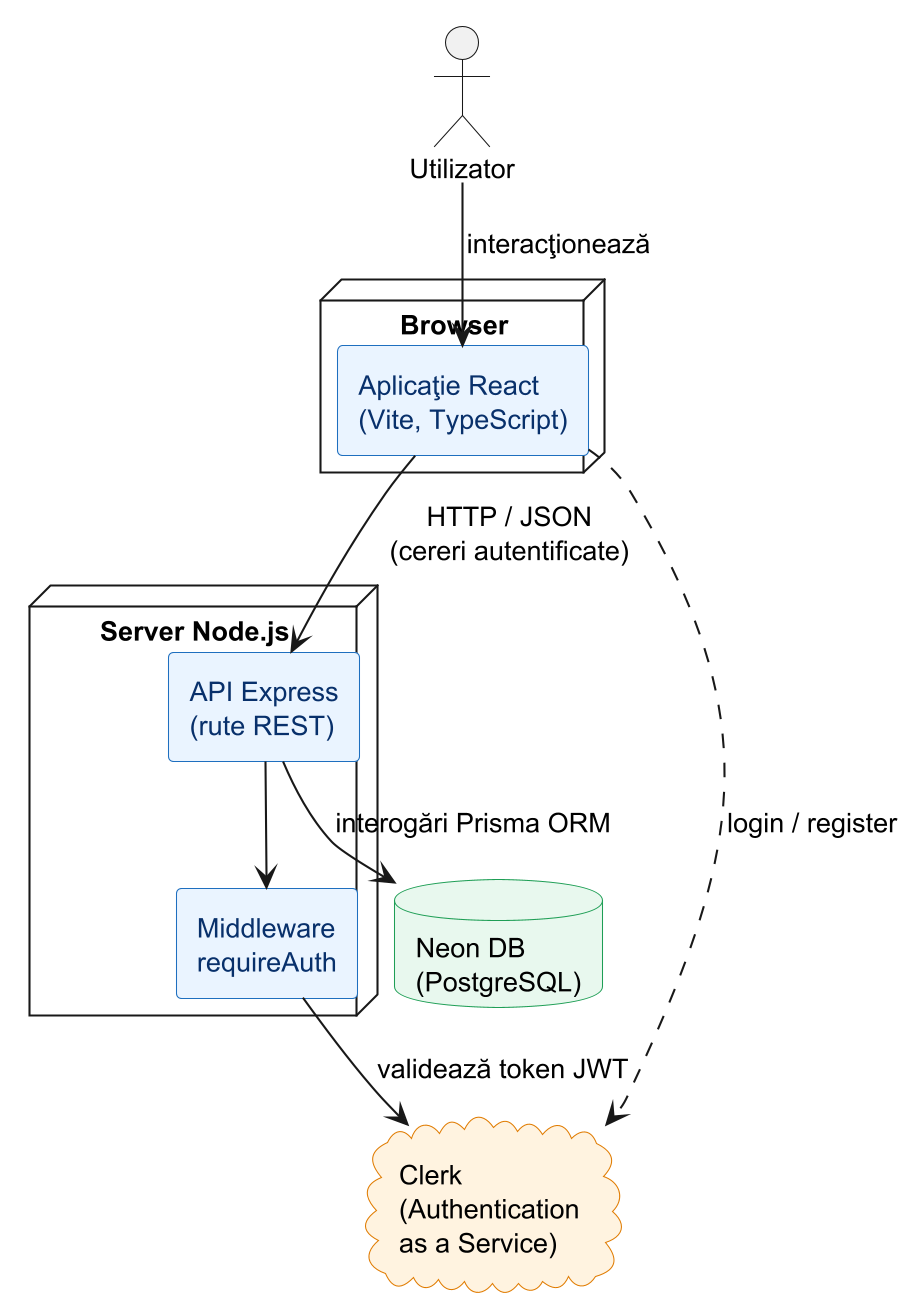
\includegraphics[width=0.72\textwidth]{arhitectura.png}
  \caption{Arhitectura general\u a a aplica\c tiei Gym-Connect}
  \label{fig:arhitectura}
\end{figure}

\begin{enumerate}
  \item \textbf{Nivelul de prezentare (Frontend)} -- aplica\c tia React
        care ruleaz\u a \^ in browserul utilizatorului. Aceasta
        gestioneaz\u a interfa\c ta utilizator, starea local\u a
        a aplica\c tiei \c si comunic\u a cu serverul prin cereri
        HTTP autentificate.

  \item \textbf{Nivelul de logic\u a de business (Backend)} -- serverul
        Express.js care ruleaz\u a pe Node.js. Acesta prime\c ste
        cererile de la client, le valideaz\u a, aplic\u a logica
        de business \c si interac\c tioneaz\u a cu baza de date
        prin Prisma ORM.

  \item \textbf{Nivelul de date (Baza de date)} -- instan\c ta
        PostgreSQL g\u azduit\u a pe platforma Neon DB. Stocheaz\u a
        toate datele aplica\c tiei: rutine de antrenament,
        sesiuni \c si seturi individuale.
\end{enumerate}

Fluxul standard al unei cereri este urm\u atorul: browserul
utilizatorului trimite o cerere HTTP c\u atre serverul Express,
\^ inso\c tit\u a de un token de autentificare Clerk. Serverul
valideaz\u a tokenul, proceseaz\u a cererea, interogheaz\u a
baza de date prin Prisma \c si returneaz\u a r\u aspunsul \^ in
format JSON c\u atre client.

\^ In modul de dezvoltare, Vite ofer\u a un \textbf{proxy} c\u atre
serverul backend, astfel \^ inc\^ at cererile de pe
\texttt{localhost:5173/api/*} sunt redirijate automat c\u atre
\texttt{localhost:3001/api/*}, evit\^ and problemele de CORS \^ in
timpul dezvolt\u arii.

\section{Modelul de date}

Schema bazei de date este definit\u a declarativ \^ in fi\c sierul
\texttt{prisma/schema.prisma} \c si este compus\u a din trei modele
principale, interconectate prin rela\c tii de tip
\textit{one-to-many}.

\subsection{Modelul SplitTemplate}

Modelul \texttt{SplitTemplate} reprezint\u a un \textbf{\c sablon de
rutin\u a de antrenament} -- un plan predefinit care descrie ce
exerci\c tii, c\^ ate seturi \c si ce interval de repeti\c tii
trebuie efectuate. Un utilizator poate crea oric\^ ate rutine,
iar fiecare rutin\u a apar\c tine exclusiv utilizatorului care
a creat-o.

\begin{table}[htbp]
\centering
\caption{C\^ ampurile modelului \texttt{SplitTemplate}}
\label{tab:split}
\begin{tabular}{|l|l|l|}
\hline
\textbf{C\^ amp} & \textbf{Tip} & \textbf{Descriere} \\
\hline
\texttt{id}          & String (CUID) & Identificator unic generat automat \\
\texttt{userId}      & String        & ID-ul utilizatorului proprietar (Clerk) \\
\texttt{name}        & String        & Numele rutinei \\
\texttt{description} & String        & Descriere op\c tional\u a \\
\texttt{exercises}   & JSON          & Lista exerci\c tiilor cu seturi \c si repeti\c tii \\
\texttt{createdAt}   & DateTime      & Data cre\u arii \\
\texttt{updatedAt}   & DateTime      & Data ultimei modific\u ari \\
\hline
\end{tabular}
\end{table}

C\^ ampul \texttt{exercises} stocheaz\u a o structur\u a JSON care
con\c tine un array de obiecte, fiecare descriind un exerci\c tiu
din rutin\u a cu urm\u atoarele propriet\u a\c ti:
\texttt{exerciseId} (identificatorul exerci\c tiului din baza de
date local\u a), \texttt{targetSets} (num\u arul de seturi
\c tint\u a), \texttt{targetRepRange} (intervalul de repeti\c tii,
ex. \textit{8--12}) \c si \texttt{order} (ordinea exerci\c tiului
\^ in rutin\u a). Alegerea stoc\u arii \^ in format JSON a fost
motivat\u a de faptul c\u a structura exerci\c tiilor dintr-o
rutin\u a este variat\u a \c si nu necesit\u a interog\u ari
rela\c tionale independente.

\subsection{Modelul WorkoutSession}

Modelul \texttt{WorkoutSession} reprezint\u a o \textbf{sesiune de
antrenament efectuat\u a} -- o \^ inregistrare a unui antrenament
real, cu data, durata \c si seturile efectuate. Fiecare sesiune
poate fi op\c tional asociat\u a cu o rutin\u a de antrenament
(\texttt{SplitTemplate}), dar poate exista \c si independent
(antrenament liber). Rela\c tia cu \texttt{SplitTemplate} este
de tip \textit{many-to-one}, cu comportament \texttt{SetNull}
la \c stergere -- dac\u a o rutin\u a este \c stears\u a,
sesiunile asociate nu sunt \c sterse, ci r\u am\^ an cu
\texttt{splitId = null}.

\begin{table}[htbp]
\centering
\caption{C\^ ampurile modelului \texttt{WorkoutSession}}
\label{tab:session}
\begin{tabular}{|l|l|l|}
\hline
\textbf{C\^ amp} & \textbf{Tip} & \textbf{Descriere} \\
\hline
\texttt{id}              & String (CUID) & Identificator unic \\
\texttt{userId}          & String        & ID-ul utilizatorului (Clerk) \\
\texttt{splitId}         & String?       & Referin\c t\u a op\c tional\u a la rutin\u a \\
\texttt{splitName}       & String        & Numele rutinei la momentul sesiunii \\
\texttt{date}            & DateTime      & Data \c si ora antrenamentului \\
\texttt{durationSeconds} & Int           & Durata \^ in secunde \\
\texttt{notes}           & String?       & Note op\c tionale \\
\texttt{createdAt}       & DateTime      & Data \^ inregistr\u arii \\
\hline
\end{tabular}
\end{table}

C\^ ampul \texttt{splitName} stocheaz\u a numele rutinei la momentul
efectu\u arii sesiunii. Aceast\u a decizie de proiectare asigur\u a
c\u a istoricul r\u am\^ ane corect chiar dac\u a utilizatorul
redenume\c ste sau \c sterge rutina ulterior.

\subsection{Modelul WorkoutSet}

Modelul \texttt{WorkoutSet} reprezint\u a \textbf{un set individual}
dintr-o sesiune de antrenament -- cea mai granular\u a unitate de
date a aplica\c tiei. Fiecare sesiune con\c tine unul sau mai multe
seturi, fiecare corespunz\^ and unui exerci\c tiu specific. Rela\c tia
cu \texttt{WorkoutSession} este de tip \textit{many-to-one} cu
comportament \texttt{Cascade} -- \c stergerea unei sesiuni
atrage \c si \c stergerea tuturor seturilor asociate.

\begin{table}[htbp]
\centering
\caption{C\^ ampurile modelului \texttt{WorkoutSet}}
\label{tab:set}
\begin{tabular}{|l|l|l|}
\hline
\textbf{C\^ amp} & \textbf{Tip} & \textbf{Descriere} \\
\hline
\texttt{id}         & String (CUID) & Identificator unic \\
\texttt{sessionId}  & String        & Referin\c t\u a la sesiunea p\u arinte \\
\texttt{exerciseId} & String        & ID-ul exerci\c tiului \\
\texttt{setOrder}   & Int           & Ordinea setului \^ in sesiune \\
\texttt{weight}     & Float         & Greutatea utilizat\u a (kg) \\
\texttt{reps}       & Int           & Num\u arul de repeti\c tii efectuate \\
\texttt{rir}        & Int           & Reps in Reserve (0--10) \\
\texttt{isWarmup}   & Boolean       & Marcaj set de \^ inc\u alzire \\
\hline
\end{tabular}
\end{table}

C\^ ampul \texttt{rir} (\textit{Reps in Reserve}) reprezint\u a
num\u arul estimat de repeti\c tii r\u amase p\^ an\u a la cedare.
Un RIR de 0 indic\u a epuizare muscular\u a complet\u a, \^ in timp
ce un RIR de 3 indic\u a c\u a sportivul putea efectua \^ inc\u a
3 repeti\c tii. Acest indicator este utilizat \^ in modulul de
analitic\u a pentru calculul 1RM estimat \c si aprecierea
intensit\u a\c tii antrenamentului.

\subsection{Rela\c tiile dintre modele}

Diagrama entitate-rela\c tie din figura \ref{fig:bazadedate} prezint\u a
structura complet\u a a bazei de date, cu cele trei modele, c\^ ampurile
lor \c si rela\c tiile dintre ele.

\begin{figure}[htbp]
  \centering
  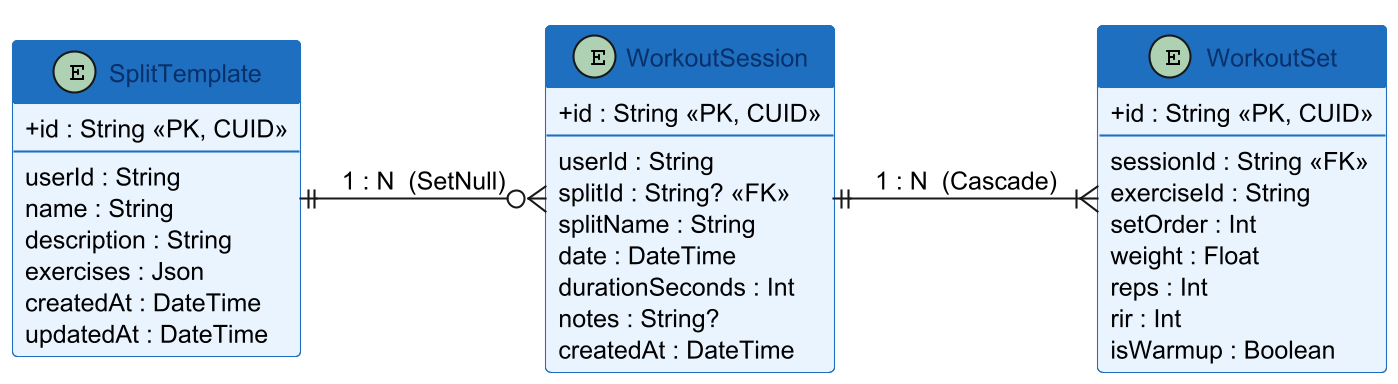
\includegraphics[width=\textwidth]{bazadedate.png}
  \caption{Diagrama entitate-rela\c tie a bazei de date}
  \label{fig:bazadedate}
\end{figure}

Cele trei modele formeaz\u a o ierarhie clar\u a:

\begin{itemize}
  \item Un utilizator (identificat prin \texttt{userId} Clerk) poate
        de\c tine orice num\u ar de \texttt{SplitTemplate}-uri \c si
        \texttt{WorkoutSession}-uri.
  \item O \texttt{WorkoutSession} poate fi asociat\u a cu cel mult
        un \texttt{SplitTemplate} (op\c tional).
  \item O \texttt{WorkoutSession} con\c tine unul sau mai multe
        \texttt{WorkoutSet}-uri.
\end{itemize}

Izolarea datelor \^ intre utilizatori este garantat\u a la nivelul
aplica\c tiei: toate interog\u arile Prisma includ filtrul
\texttt{where: \{ userId \}} extras din tokenul de autentificare
Clerk, astfel \^ inc\^ at un utilizator nu poate accesa datele
altui utilizator.

\section{API-ul REST}

Serverul Express expune un API REST cu dou\u a grupuri de endpoint-uri,
ambele protejate prin middleware-ul de autentificare Clerk.

\subsection{Endpoint-uri pentru rutine (\texttt{/api/splits})}

\begin{table}[htbp]
\centering
\caption{Endpoint-urile API pentru gestionarea rutinelor}
\label{tab:api-splits}
\begin{tabular}{|l|l|l|}
\hline
\textbf{Metod\u a} & \textbf{Rut\u a} & \textbf{Descriere} \\
\hline
GET    & \texttt{/api/splits}     & Returneaz\u a toate rutinele utilizatorului \\
POST   & \texttt{/api/splits}     & Creeaz\u a o rutin\u a nou\u a \\
PUT    & \texttt{/api/splits/:id} & Actualizeaz\u a o rutin\u a existent\u a \\
DELETE & \texttt{/api/splits/:id} & \c Sterge o rutin\u a \\
\hline
\end{tabular}
\end{table}

Endpoint-ul \texttt{POST /api/splits} valideaz\u a corpul cererii
cu schema Zod, verific\^ and c\u a rutina con\c tine un nume
nenul, o descriere op\c tional\u a \c si cel pu\c tin un exerci\c tiu
cu \texttt{exerciseId}, \texttt{targetSets} \c si
\texttt{targetRepRange} valide. Endpoint-urile
\texttt{PUT} \c si \texttt{DELETE} verific\u a suplimentar c\u a
resursa solicitat\u a apar\c tine utilizatorului curent,
return\^ and HTTP 404 \^ in caz contrar.

\subsection{Endpoint-uri pentru sesiuni (\texttt{/api/sessions})}

\begin{table}[htbp]
\centering
\caption{Endpoint-urile API pentru gestionarea sesiunilor}
\label{tab:api-sessions}
\begin{tabular}{|l|l|l|}
\hline
\textbf{Metod\u a} & \textbf{Rut\u a} & \textbf{Descriere} \\
\hline
GET  & \texttt{/api/sessions} & Returneaz\u a toate sesiunile utilizatorului \\
POST & \texttt{/api/sessions} & Salveaz\u a o sesiune nou\u a cu toate seturile \\
\hline
\end{tabular}
\end{table}

Endpoint-ul \texttt{POST /api/sessions} prime\c ste \^ intr-o
singur\u a cerere toate datele sesiunii: metadatele
(dat\u a, durat\u a, note, rutin\u a asociat\u a) \c si lista
complet\u a a seturilor efectuate. Crearea sesiunii \c si
a seturilor asociate se face \^ intr-o singur\u a tranzac\c tie
Prisma (\texttt{create} cu \texttt{sets: \{ create: [...] \}}),
garant\^ and atomicitatea opera\c tiei -- fie se salveaz\u a
totul, fie nimic.

Endpoint-ul \texttt{GET /api/sessions} returneaz\u a sesiunile
ordonate descendent dup\u a dat\u a, \^ impreun\u a cu seturile
asociate ordonate dup\u a \texttt{setOrder}.

Figura \ref{fig:secventa} ilustreaz\u a, sub forma unei diagrame de
secven\c t\u a, fluxul complet declan\c sat la salvarea unui antrenament:
de la trimiterea cererii de c\u atre client, p\^ an\u a la validarea
tokenului prin Clerk, validarea datelor cu Zod, scrierea \^ in baza de
date prin Prisma \c si returnarea r\u aspunsului.

\begin{figure}[htbp]
  \centering
  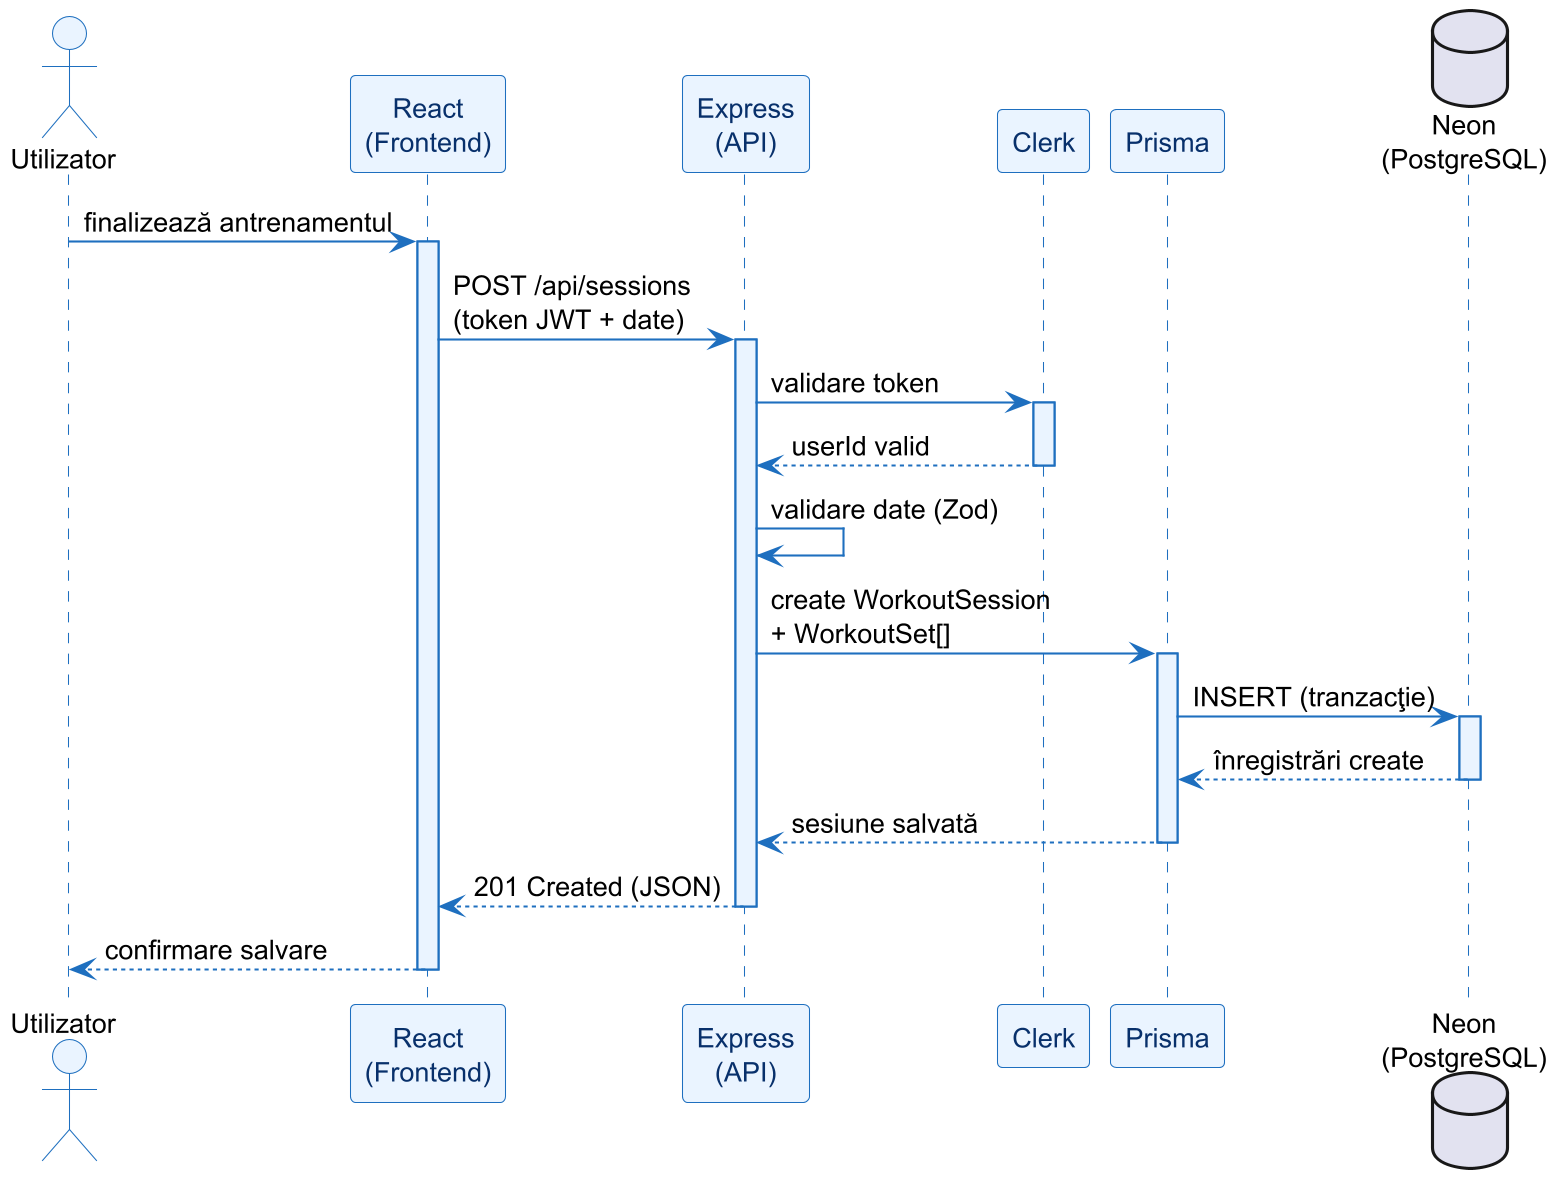
\includegraphics[width=\textwidth]{secventa.png}
  \caption{Diagrama de secven\c t\u a pentru salvarea unei sesiuni de antrenament}
  \label{fig:secventa}
\end{figure}

\section{Autentificarea \c si securitatea}

Autentificarea \^ in Gym-Connect este gestionat\u a integral
de serviciul \textbf{Clerk}, care furnizeaz\u a at\^ at
componentele UI de login/register, c\^ at \c si mecanismul
de validare a sesiunilor pe server.

\subsection{Fluxul de autentificare}

Fluxul de autentificare func\c tioneaz\u a \^ in urm\u atorii pa\c si:

\begin{enumerate}
  \item Utilizatorul se autentific\u a prin interfa\c ta Clerk
        (email + parol\u a sau OAuth).
  \item Clerk emite un \textbf{JWT} (\textit{JSON Web Token})
        semnat cu cheia privat\u a a aplica\c tiei.
  \item La fiecare cerere HTTP c\u atre server, clientul React
        include automat acest token \^ in header-ul
        \texttt{Authorization}.
  \item Pe server, middleware-ul \texttt{clerkMiddleware()}
        valideaz\u a tokenul \c si populeaz\u a obiectul cererii
        cu datele utilizatorului autentificat.
  \item Middleware-ul \texttt{requireAuth} extrage
        \texttt{userId} din cerere; dac\u a acesta lipse\c ste,
        returneaz\u a HTTP 401.
\end{enumerate}

\subsection{Middleware-ul de autentificare}

Middleware-ul \texttt{requireAuth} este aplicat global pe
toate rutele API \c si are urm\u atoarea logic\u a:

\begin{enumerate}
  \item Extrage \texttt{userId} din contextul Clerk al cererii
        curente folosind func\c tia \texttt{getAuth(req)}.
  \item Dac\u a \texttt{userId} este absent (utilizator
        neautentificat sau token expirat), returneaz\u a
        imediat r\u aspunsul \texttt{401 Unauthorized}
        cu mesajul \textit{,,Autentificare necesar\u a''}.
  \item Dac\u a autentificarea este valid\u a, adaug\u a
        \texttt{userId} pe obiectul cererii \c si transfer\u a
        controlul c\u atre handler-ul rutei.
\end{enumerate}

Prin aceast\u a abordare, nicio rut\u a API nu poate fi
accesat\u a f\u ar\u a un token valid, iar \texttt{userId}
este extras exclusiv din tokenul verificat de Clerk, nu
din parametrii cererii -- elimin\^ and posibilitatea
falsific\u arii identit\u a\c tii.

\subsection{Protec\c tia rutelor \^ in frontend}

\^ In frontend, rutele private sunt protejate prin componenta
\texttt{ProtectedRoute}, care utilizeaz\u a hook-ul
\texttt{useAuth()} al Clerk pentru a verifica starea de
autentificare. Dac\u a utilizatorul nu este autentificat,
este redirijat automat c\u atre pagina de autentificare.
\^ In caz contrar, componenta afi\c seaz\u a con\c tinutul
paginii solicitate.

\section{Diagrama cazurilor de utilizare}

Pentru a sintetiza interac\c tiunile posibile dintre utilizator \c si
aplica\c tie, figura \ref{fig:usecase} prezint\u a diagrama cazurilor
de utilizare (\textit{use-case}). Aceasta distinge \^ intre dou\u a
tipuri de actori: utilizatorul neautentificat, care poate doar s\u a
\^ i\c si creeze un cont sau s\u a se autentifice, \c si utilizatorul
autentificat, care are acces la \^ intreaga func\c tionalitate a
aplica\c tiei.

\begin{figure}[htbp]
  \centering
  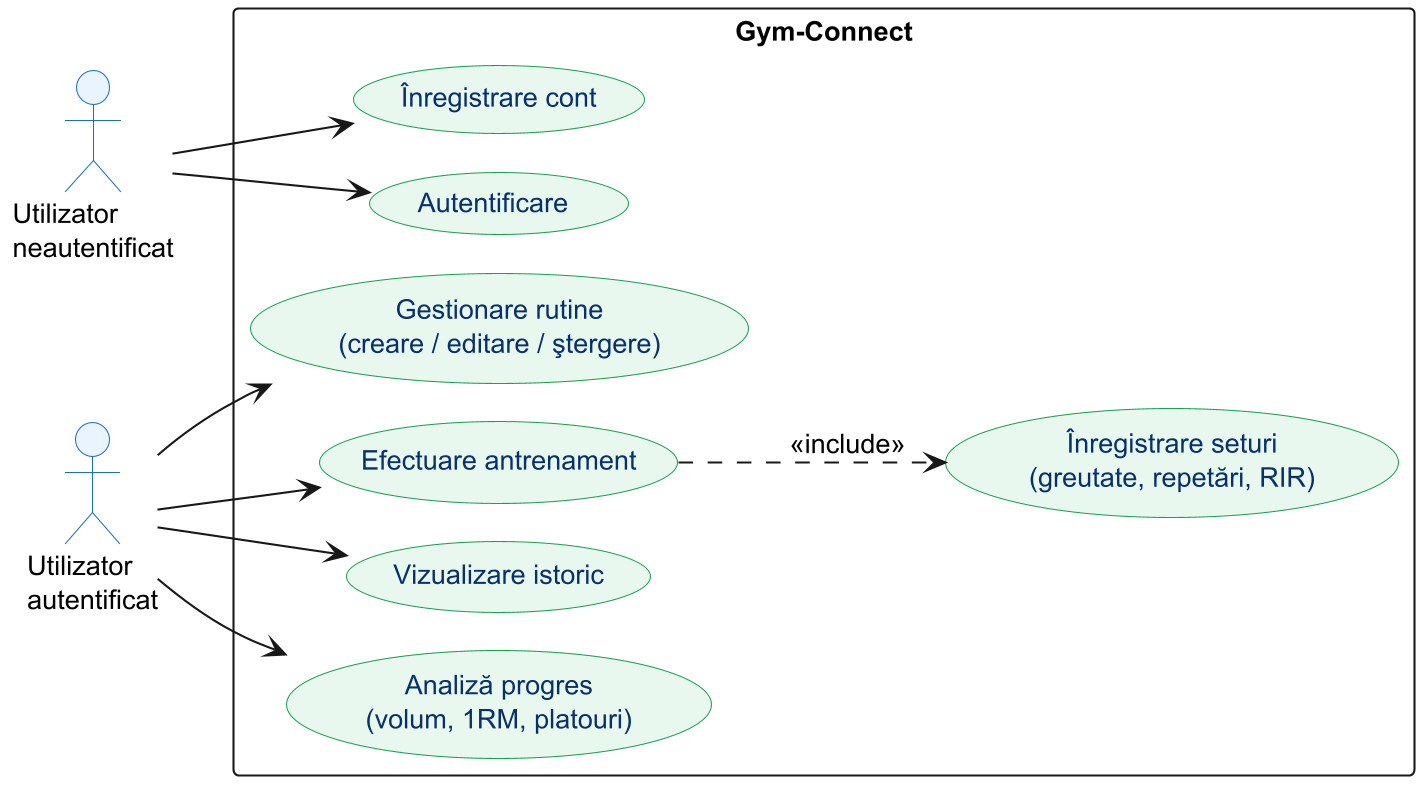
\includegraphics[width=\textwidth]{usecase.png}
  \caption{Diagrama cazurilor de utilizare a aplica\c tiei Gym-Connect}
  \label{fig:usecase}
\end{figure}

Dup\u a autentificare, utilizatorul poate gestiona rutine de
antrenament (creare, editare, \c stergere), poate efectua un
antrenament -- caz care include obligatoriu \^ inregistrarea
seturilor cu greutate, repeti\c tii \c si RIR -- poate vizualiza
istoricul sesiunilor anterioare \c si poate analiza progresul
prin intermediul modulului de analitic\u a.

     % Cap. 4 - Solutia propusa si arhitectura
\chapter{Prezentarea aplica\c tiei}

Acest capitol parcurge aplica\c tia a\c sa cum o vede un utilizator real, de
la prima pagin\u a p\^ an\u a la modulul de analiz\u a. Pentru fiecare ecran am
inclus o captur\u a din versiunea func\c tional\u a, \^ inso\c tit\u a de o scurt\u a
descriere a rolului s\u au \c si a modului de utilizare. Toate capturile provin
din aplica\c tia rulat\u a local, cu date reale de antrenament.

\section{Pagina de start (Landing Page)}

Prima pagin\u a pe care o vede un vizitator neautentificat este prezentat\u a
\^ in figura~\ref{fig:landing}. Aceasta explic\u a pe scurt ce face aplica\c tia
\c si ofer\u a butoanele de autentificare \c si \^ inregistrare. Am p\u astrat-o
deliberat simpl\u a \c si direct\u a -- scopul ei este doar s\u a conduc\u a
vizitatorul c\u atre crearea unui cont.

\begin{figure}[H]
  \centering
  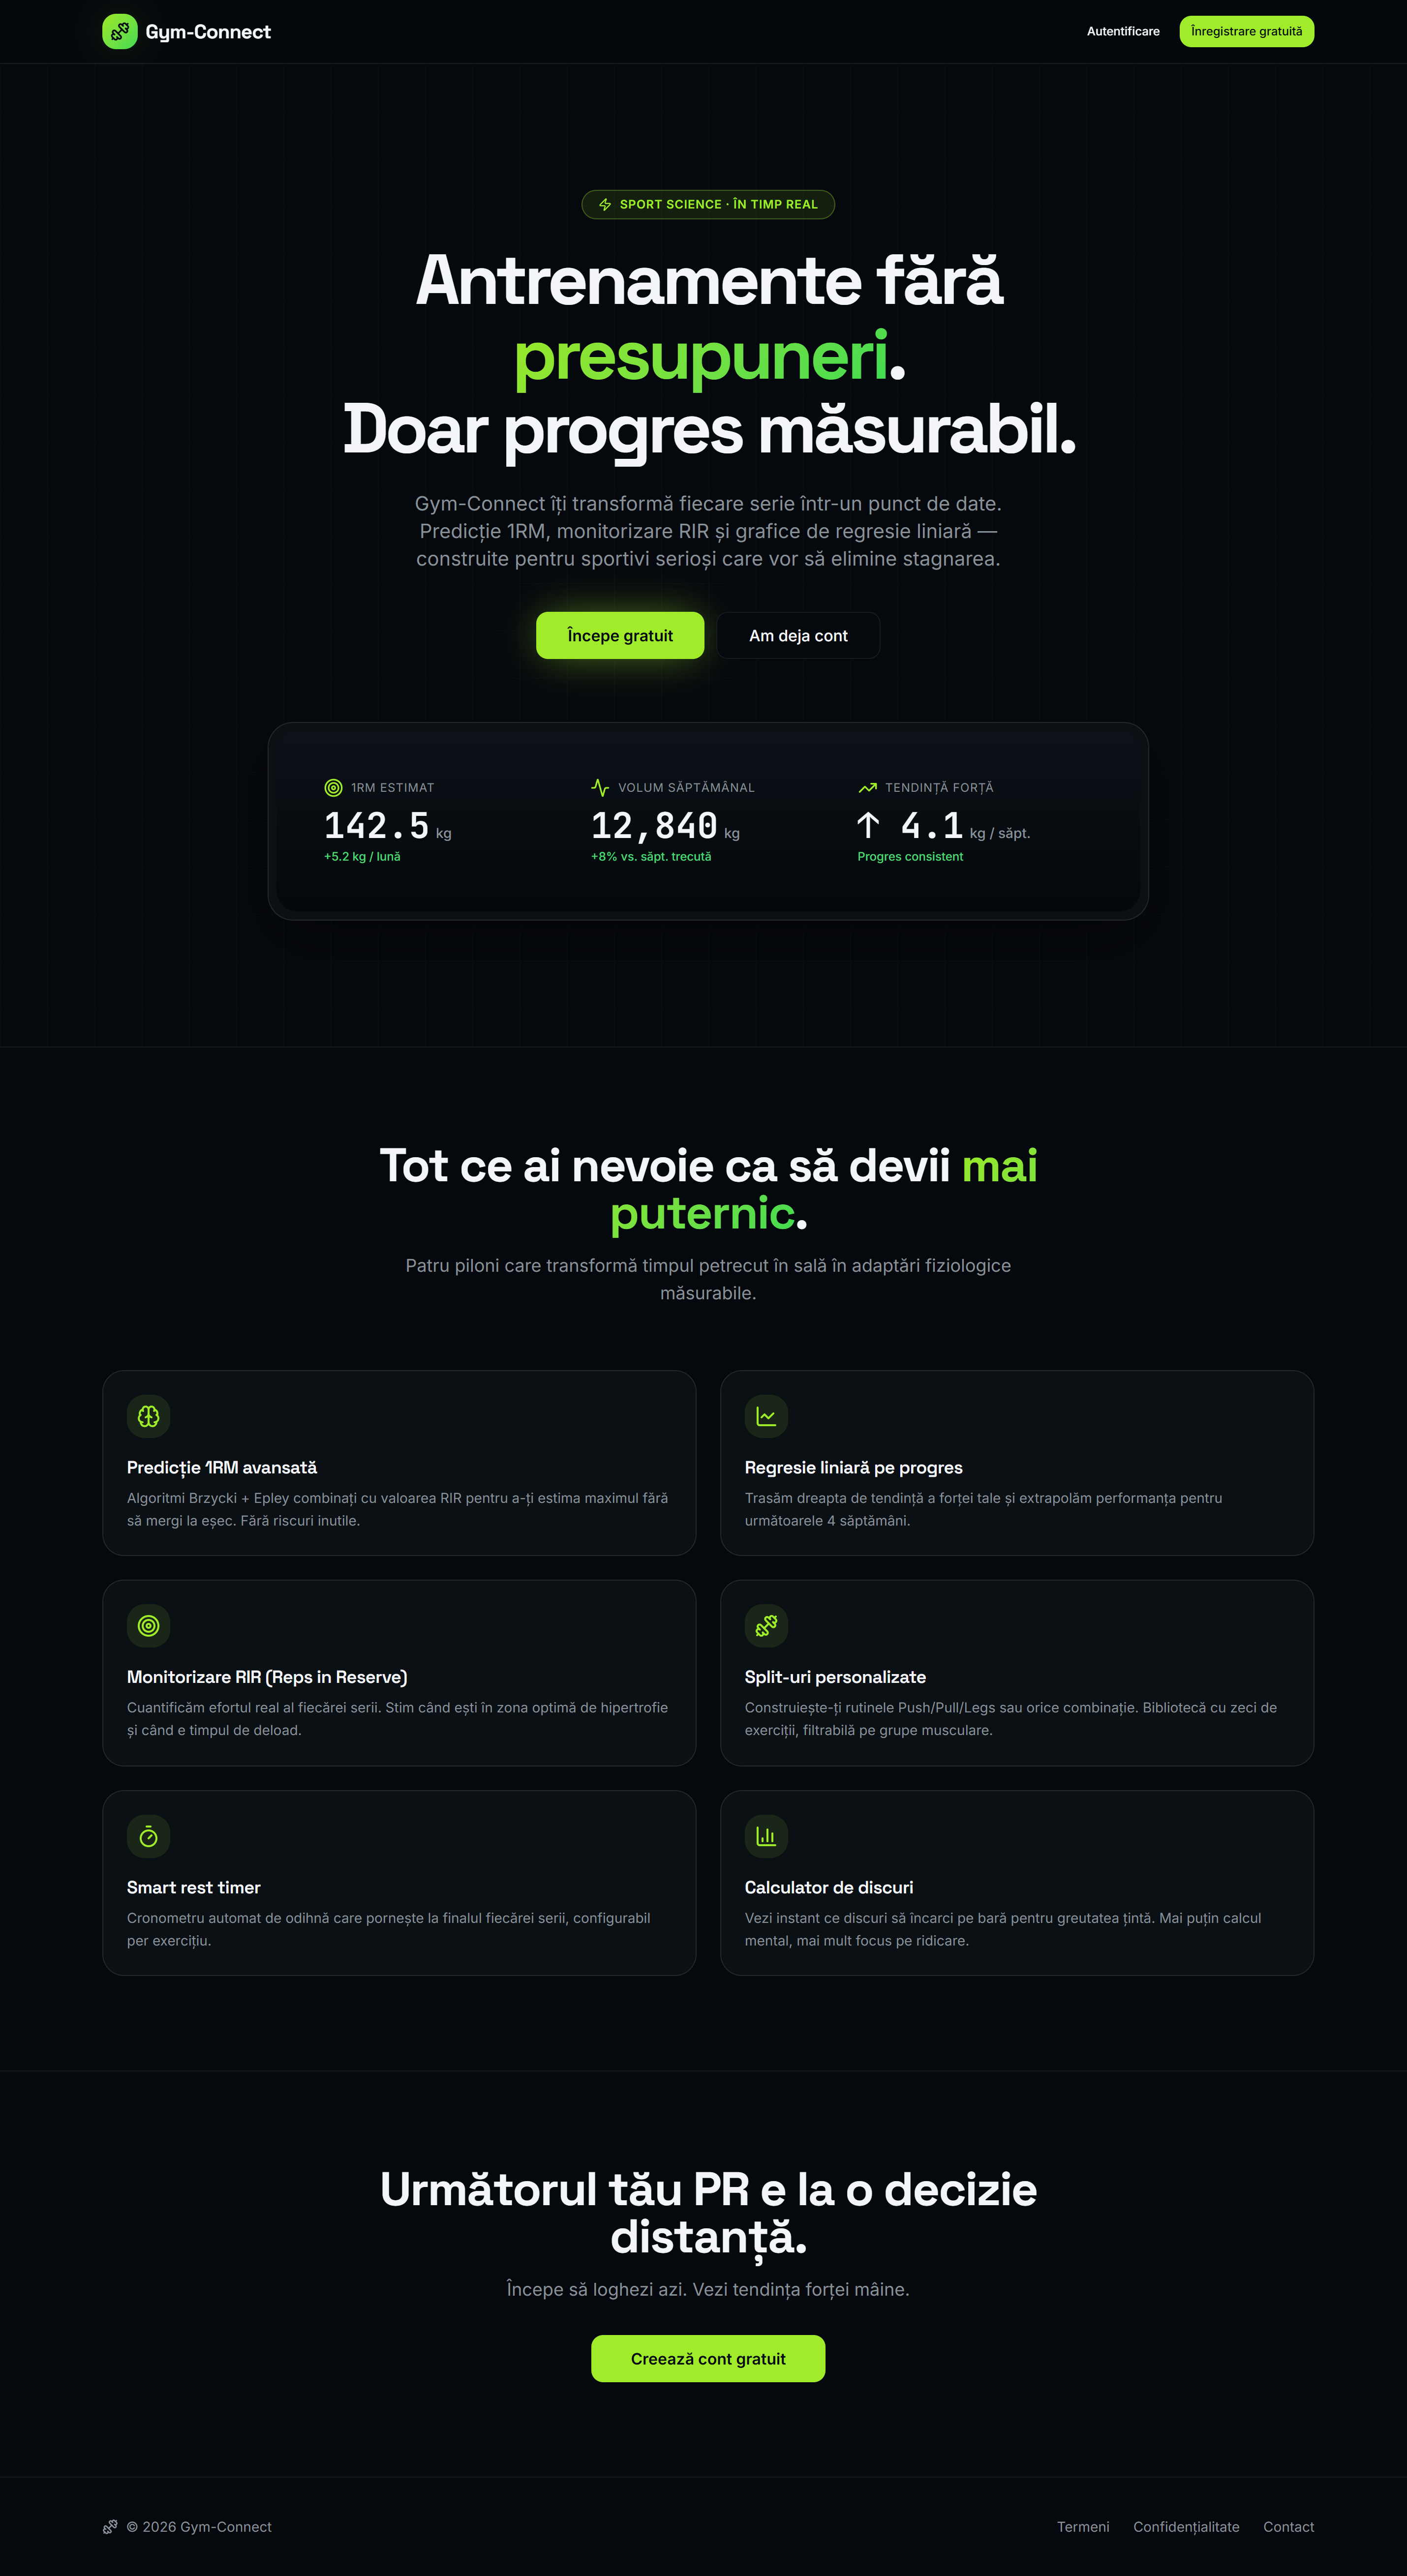
\includegraphics[height=0.78\textheight]{landing.png}
  \caption{Pagina de start (Landing Page)}
  \label{fig:landing}
\end{figure}

\section{Autentificare \c si \^ inregistrare}

Autentificarea \c si \^ inregistrarea sunt gestionate integral de Clerk, prin
componentele sale predefinite. Figura~\ref{fig:login} prezint\u a pagina de
autentificare, unde utilizatorul \^ i\c si introduce email-ul \c si parola sau
folose\c ste un cont social. Toat\u a logica sensibil\u a -- validarea parolei
\c si gestionarea sesiunii -- r\u am\^ ane \^ in sarcina Clerk.

\begin{figure}[H]
  \centering
  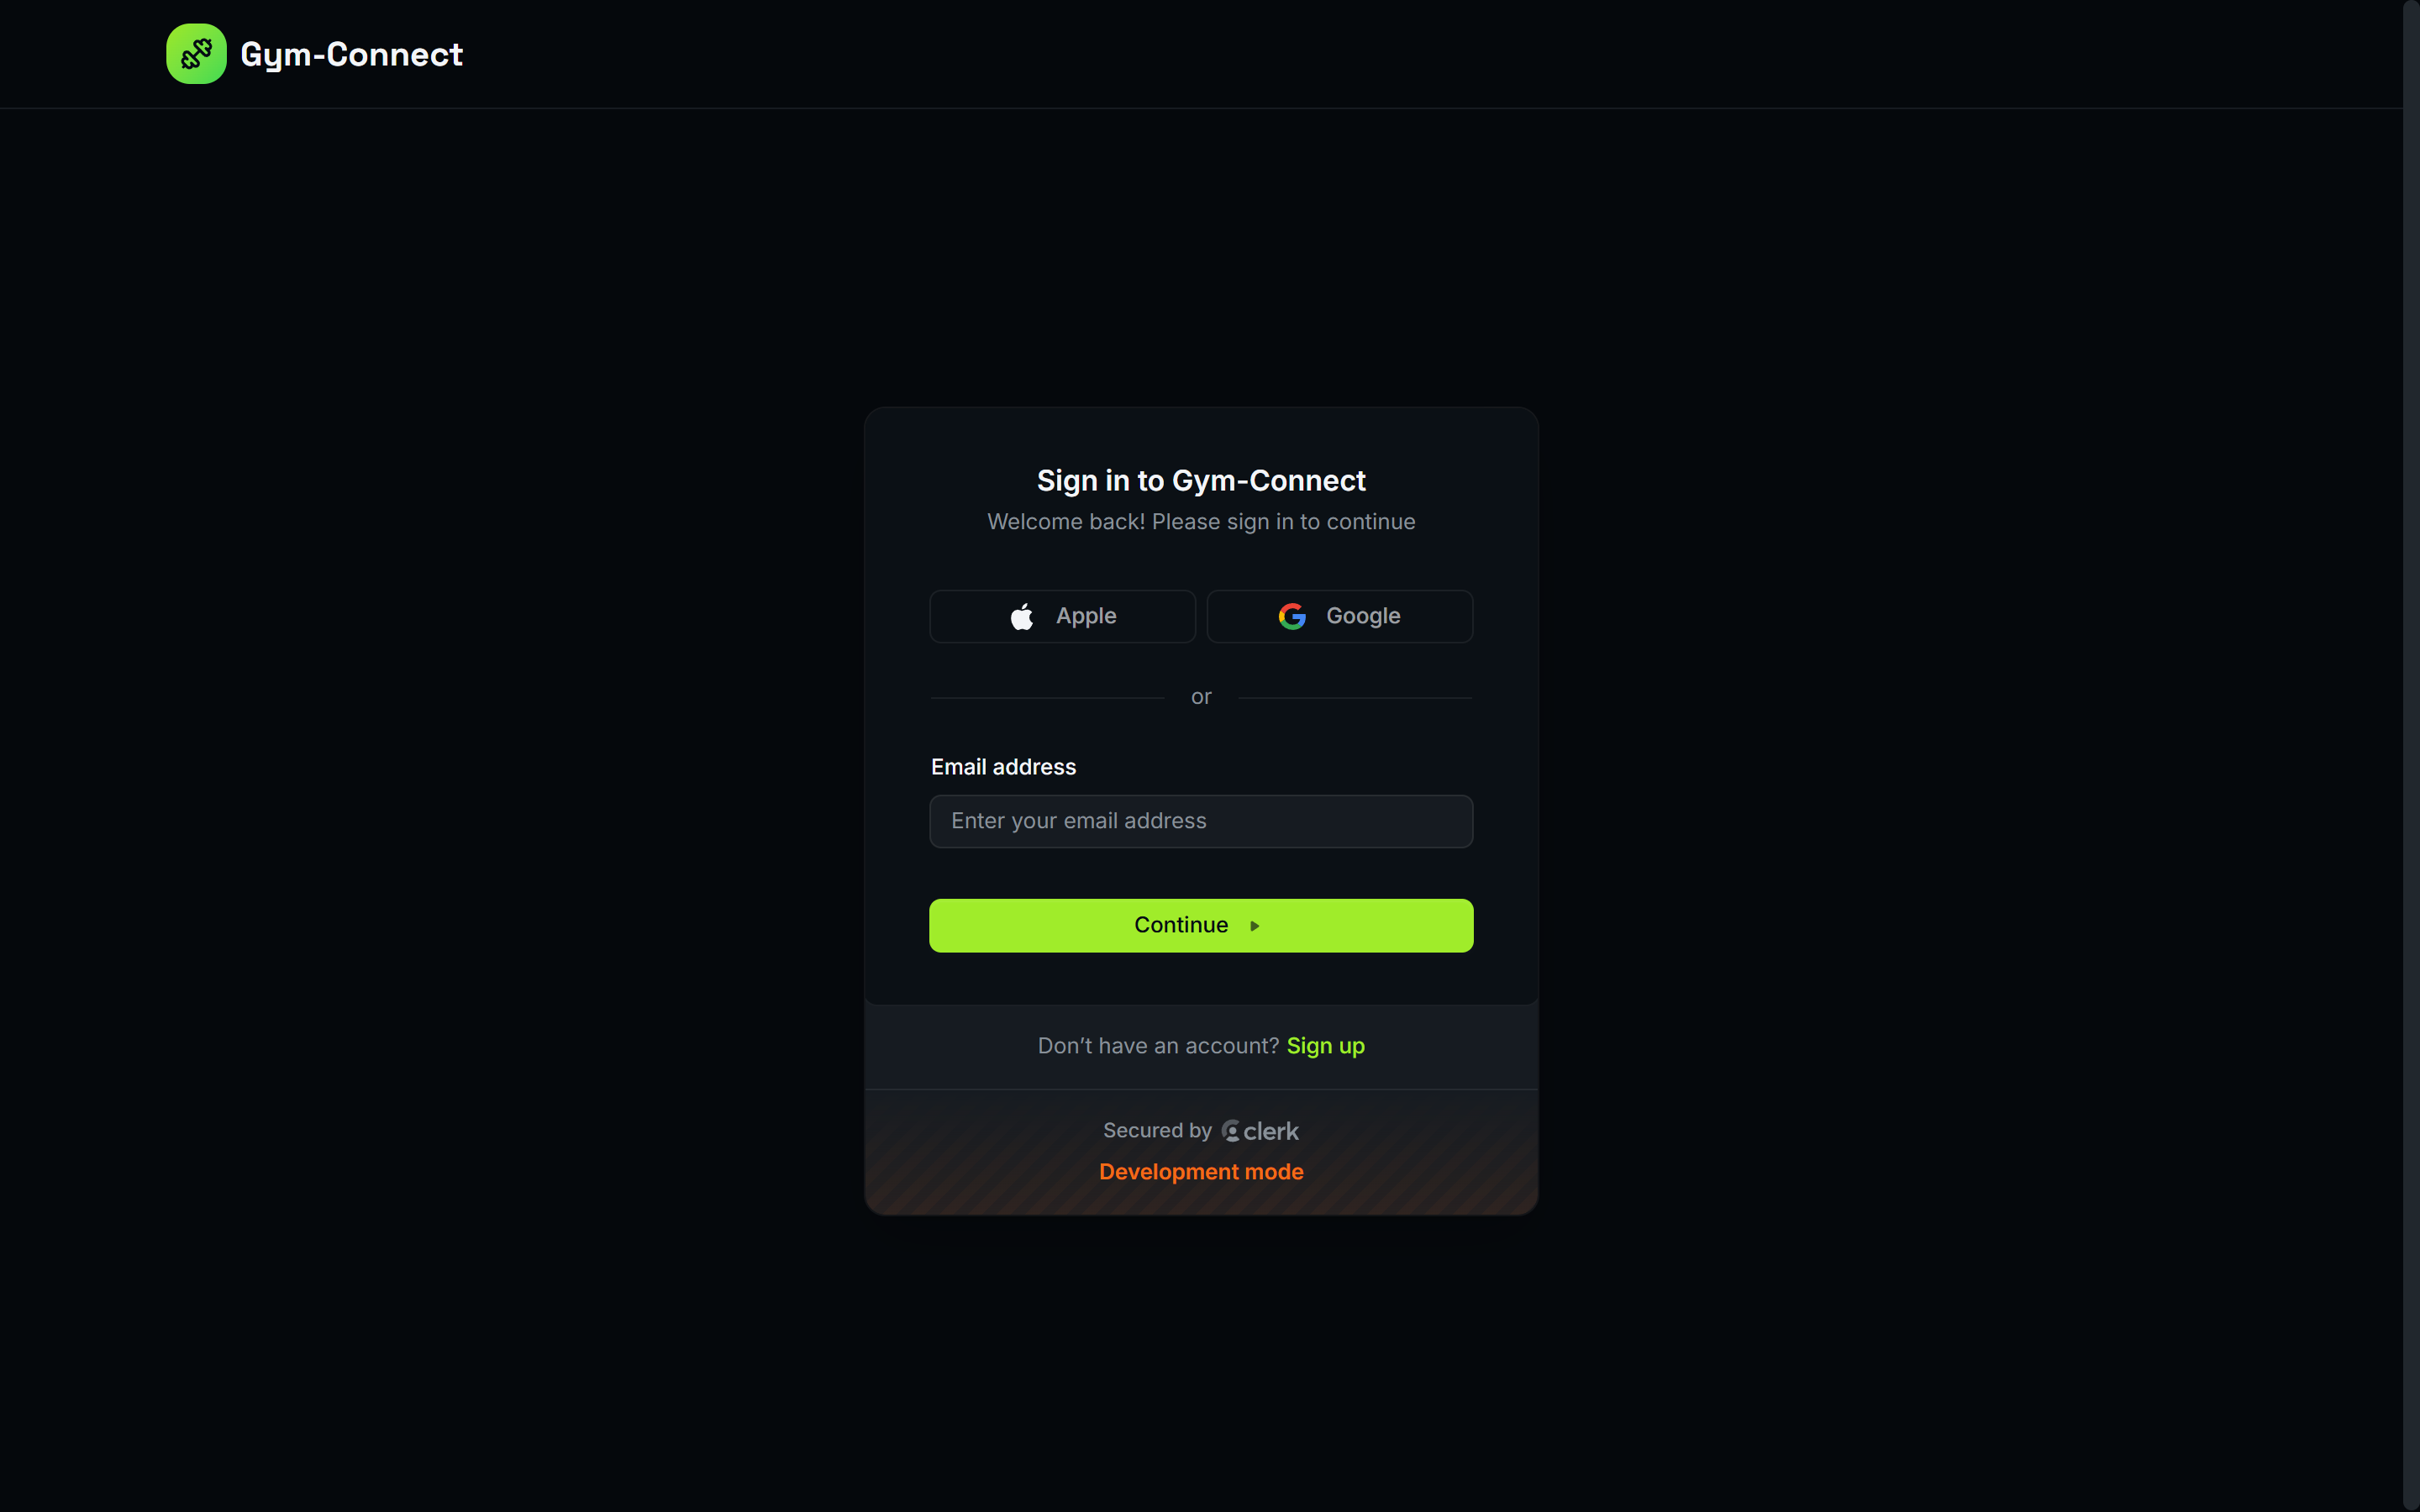
\includegraphics[width=\textwidth]{login.png}
  \caption{Pagina de autentificare}
  \label{fig:login}
\end{figure}

Pagina de \^ inregistrare, ilustrat\u a \^ in figura~\ref{fig:register}, urmeaz\u a
acela\c si tipar. Un utilizator nou \^ i\c si creeaz\u a contul \^ in c\^ ateva
secunde, iar din acel moment toate datele lui de antrenament vor fi legate de
identificatorul unic primit de la Clerk.

\begin{figure}[H]
  \centering
  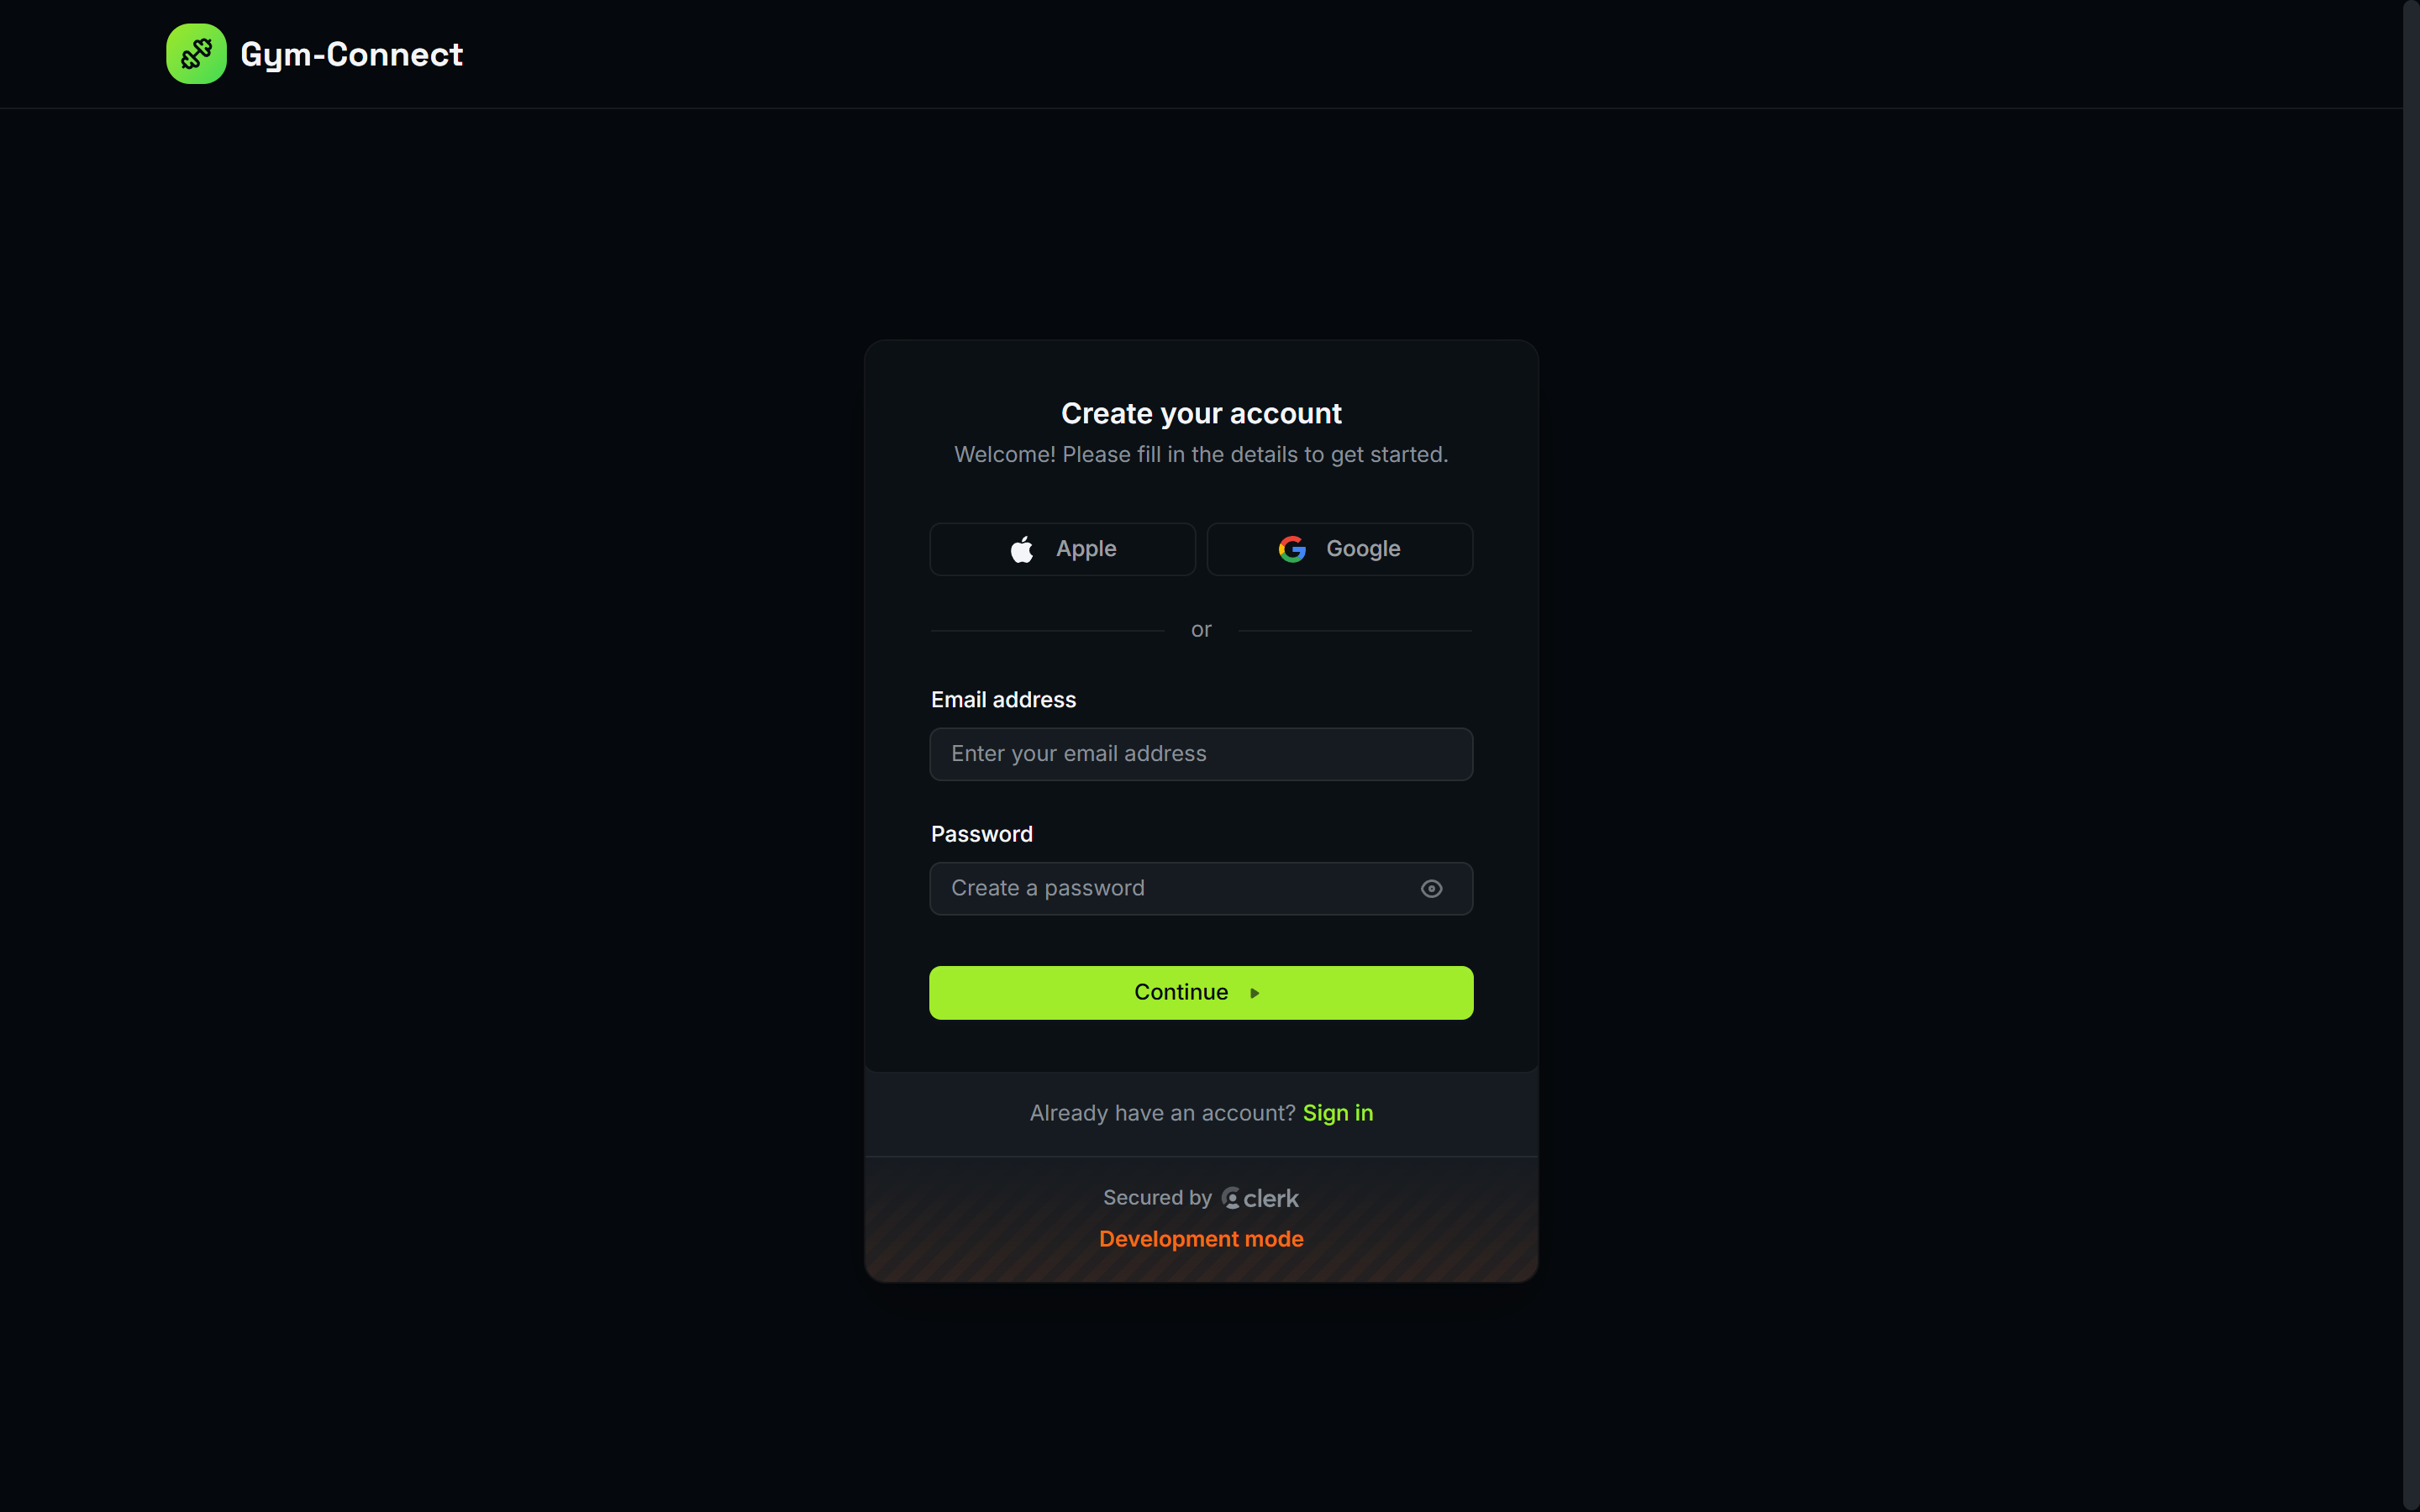
\includegraphics[width=\textwidth]{register.png}
  \caption{Pagina de \^ inregistrare}
  \label{fig:register}
\end{figure}

\section{Gestionarea rutinelor (Splits)}

Dup\u a autentificare, utilizatorul ajunge la pagina de rutine
(figura~\ref{fig:splits}). Aici sunt afi\c sate toate \c sabloanele de
antrenament salvate, fiecare cu exerci\c tiile sale. De pe acest ecran se
poate crea o rutin\u a nou\u a, edita sau \c sterge una existent\u a, ori porni
direct un antrenament.

\begin{figure}[H]
  \centering
  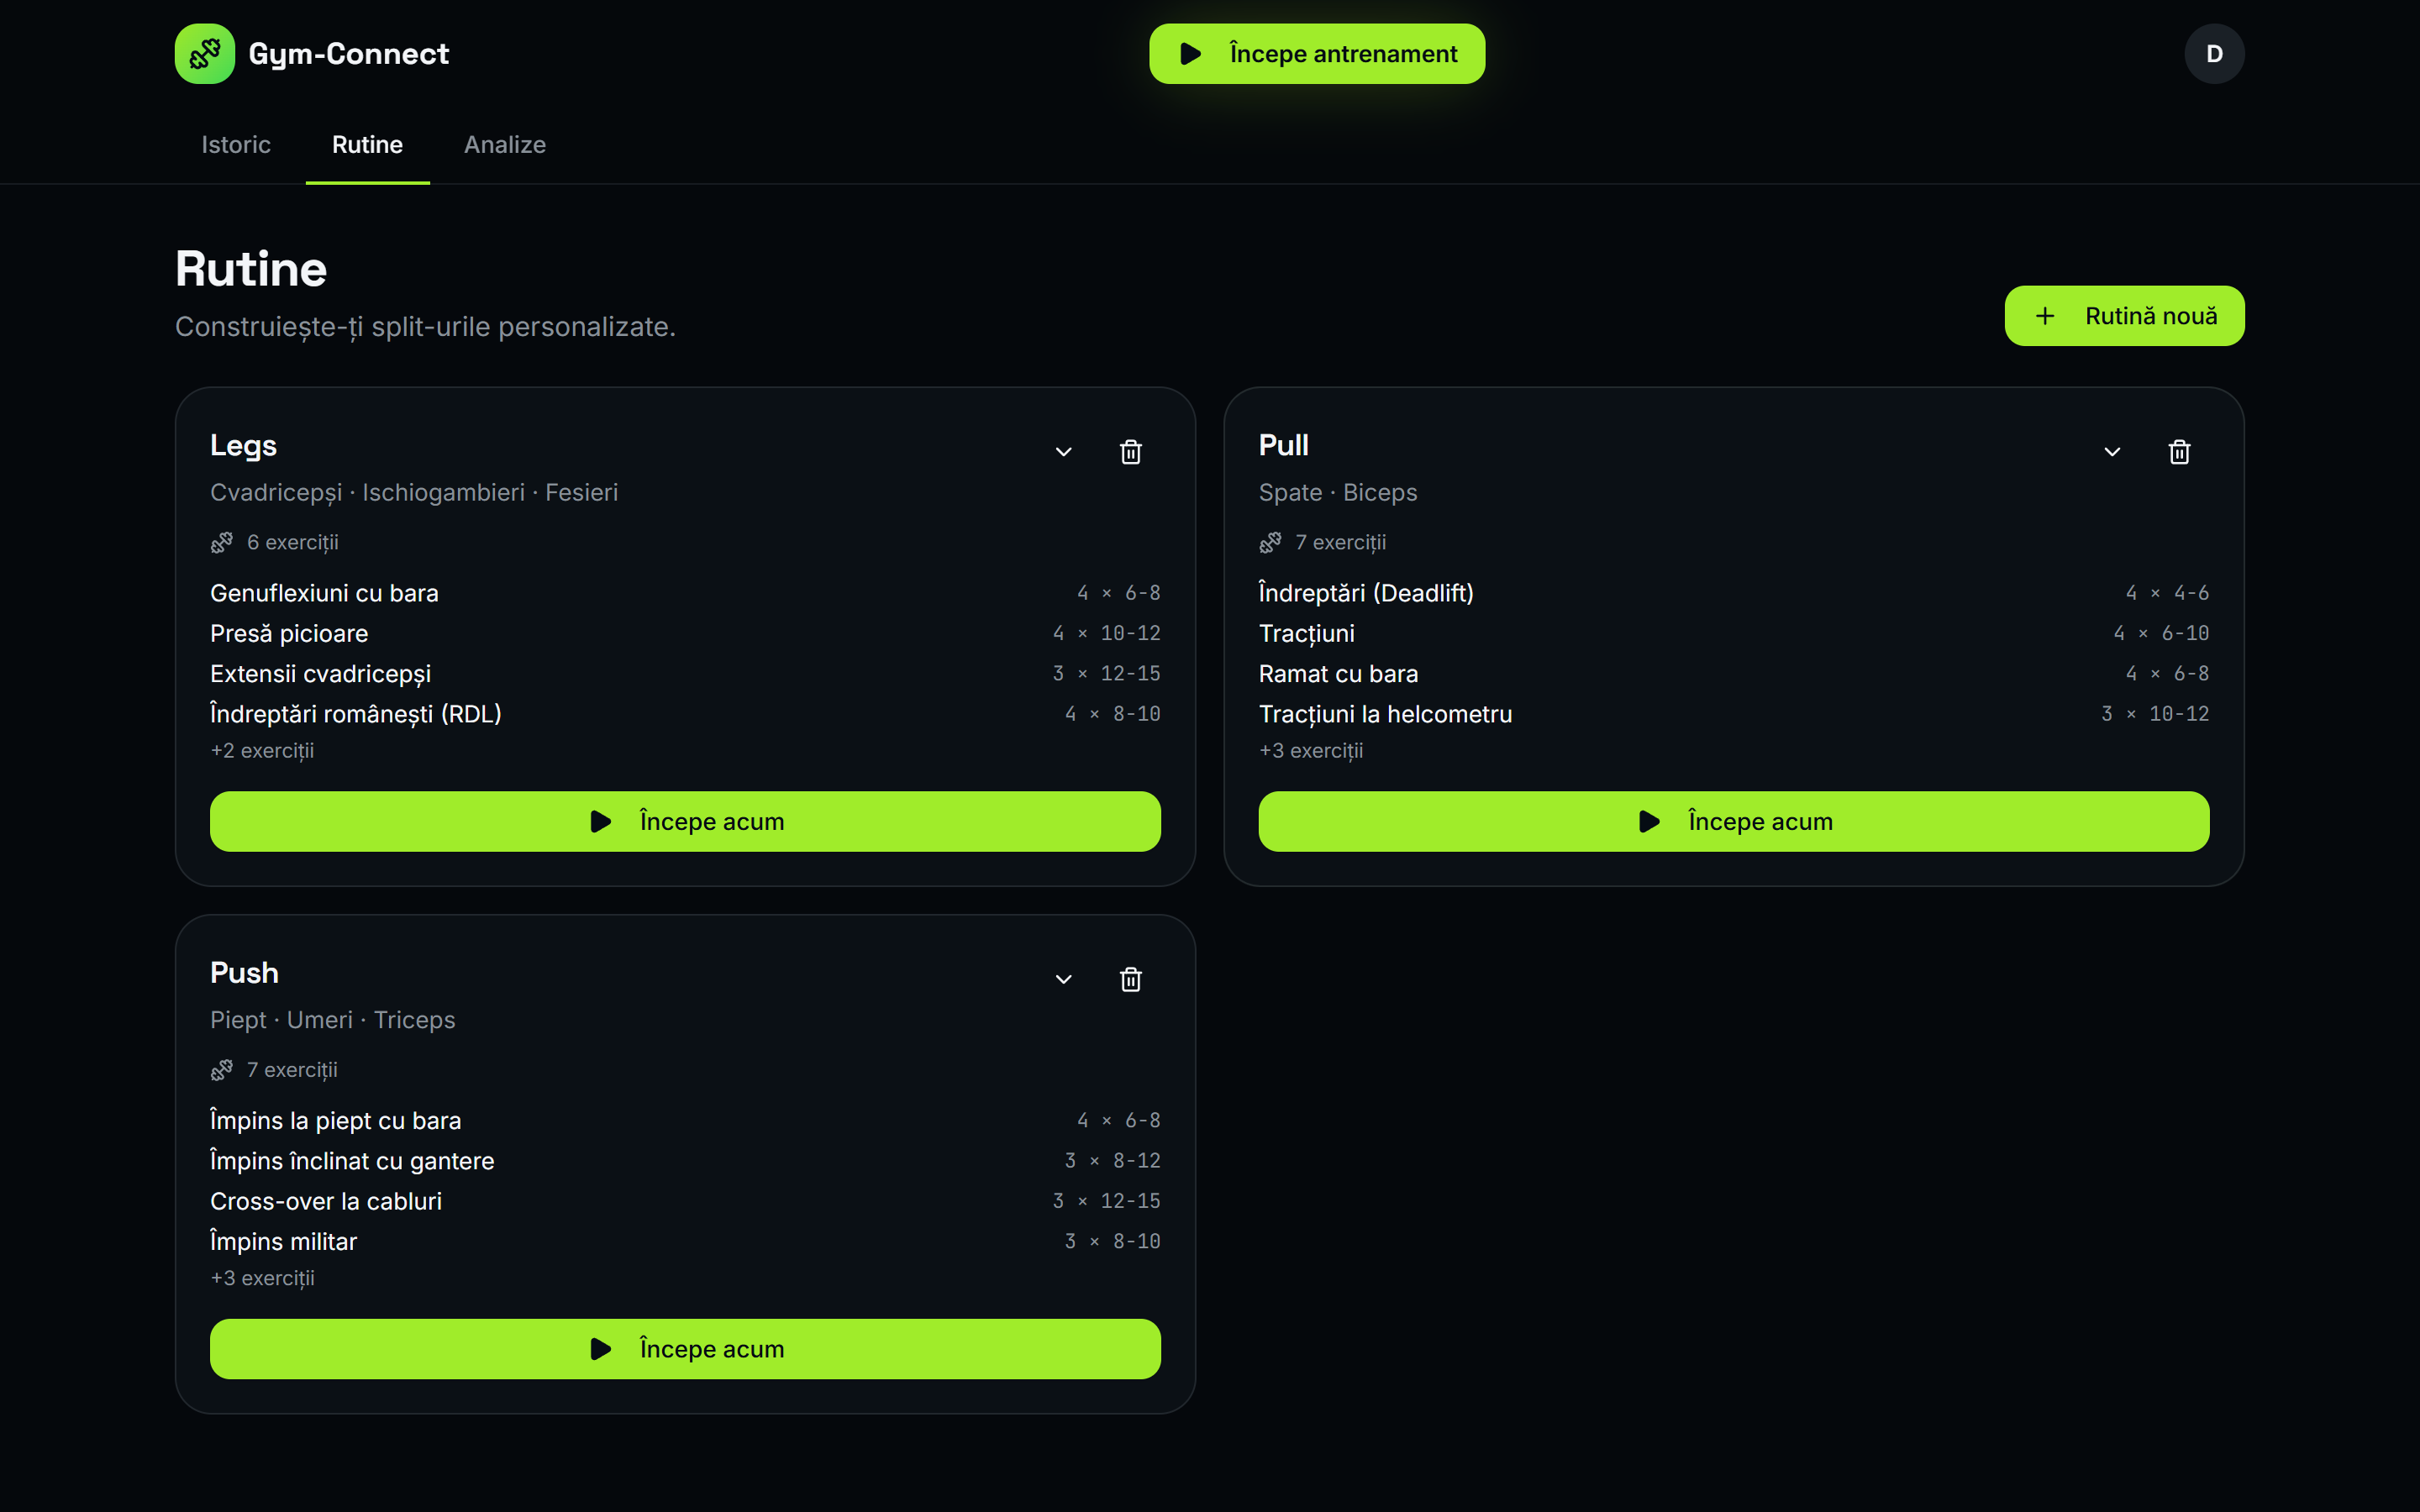
\includegraphics[width=\textwidth]{splits.png}
  \caption{Pagina de gestionare a rutinelor}
  \label{fig:splits}
\end{figure}

\subsection{Crearea unei rutine}

Crearea unei rutine se face \^ intr-un formular dedicat
(figura~\ref{fig:split-create}), \^ in care utilizatorul d\u a un nume rutinei,
o descriere op\c tional\u a \c si adaug\u a exerci\c tii. Pentru fiecare exerci\c tiu
se stabilesc num\u arul de seturi \c tint\u a \c si intervalul de repeti\c tii dorit.

\begin{figure}[H]
  \centering
  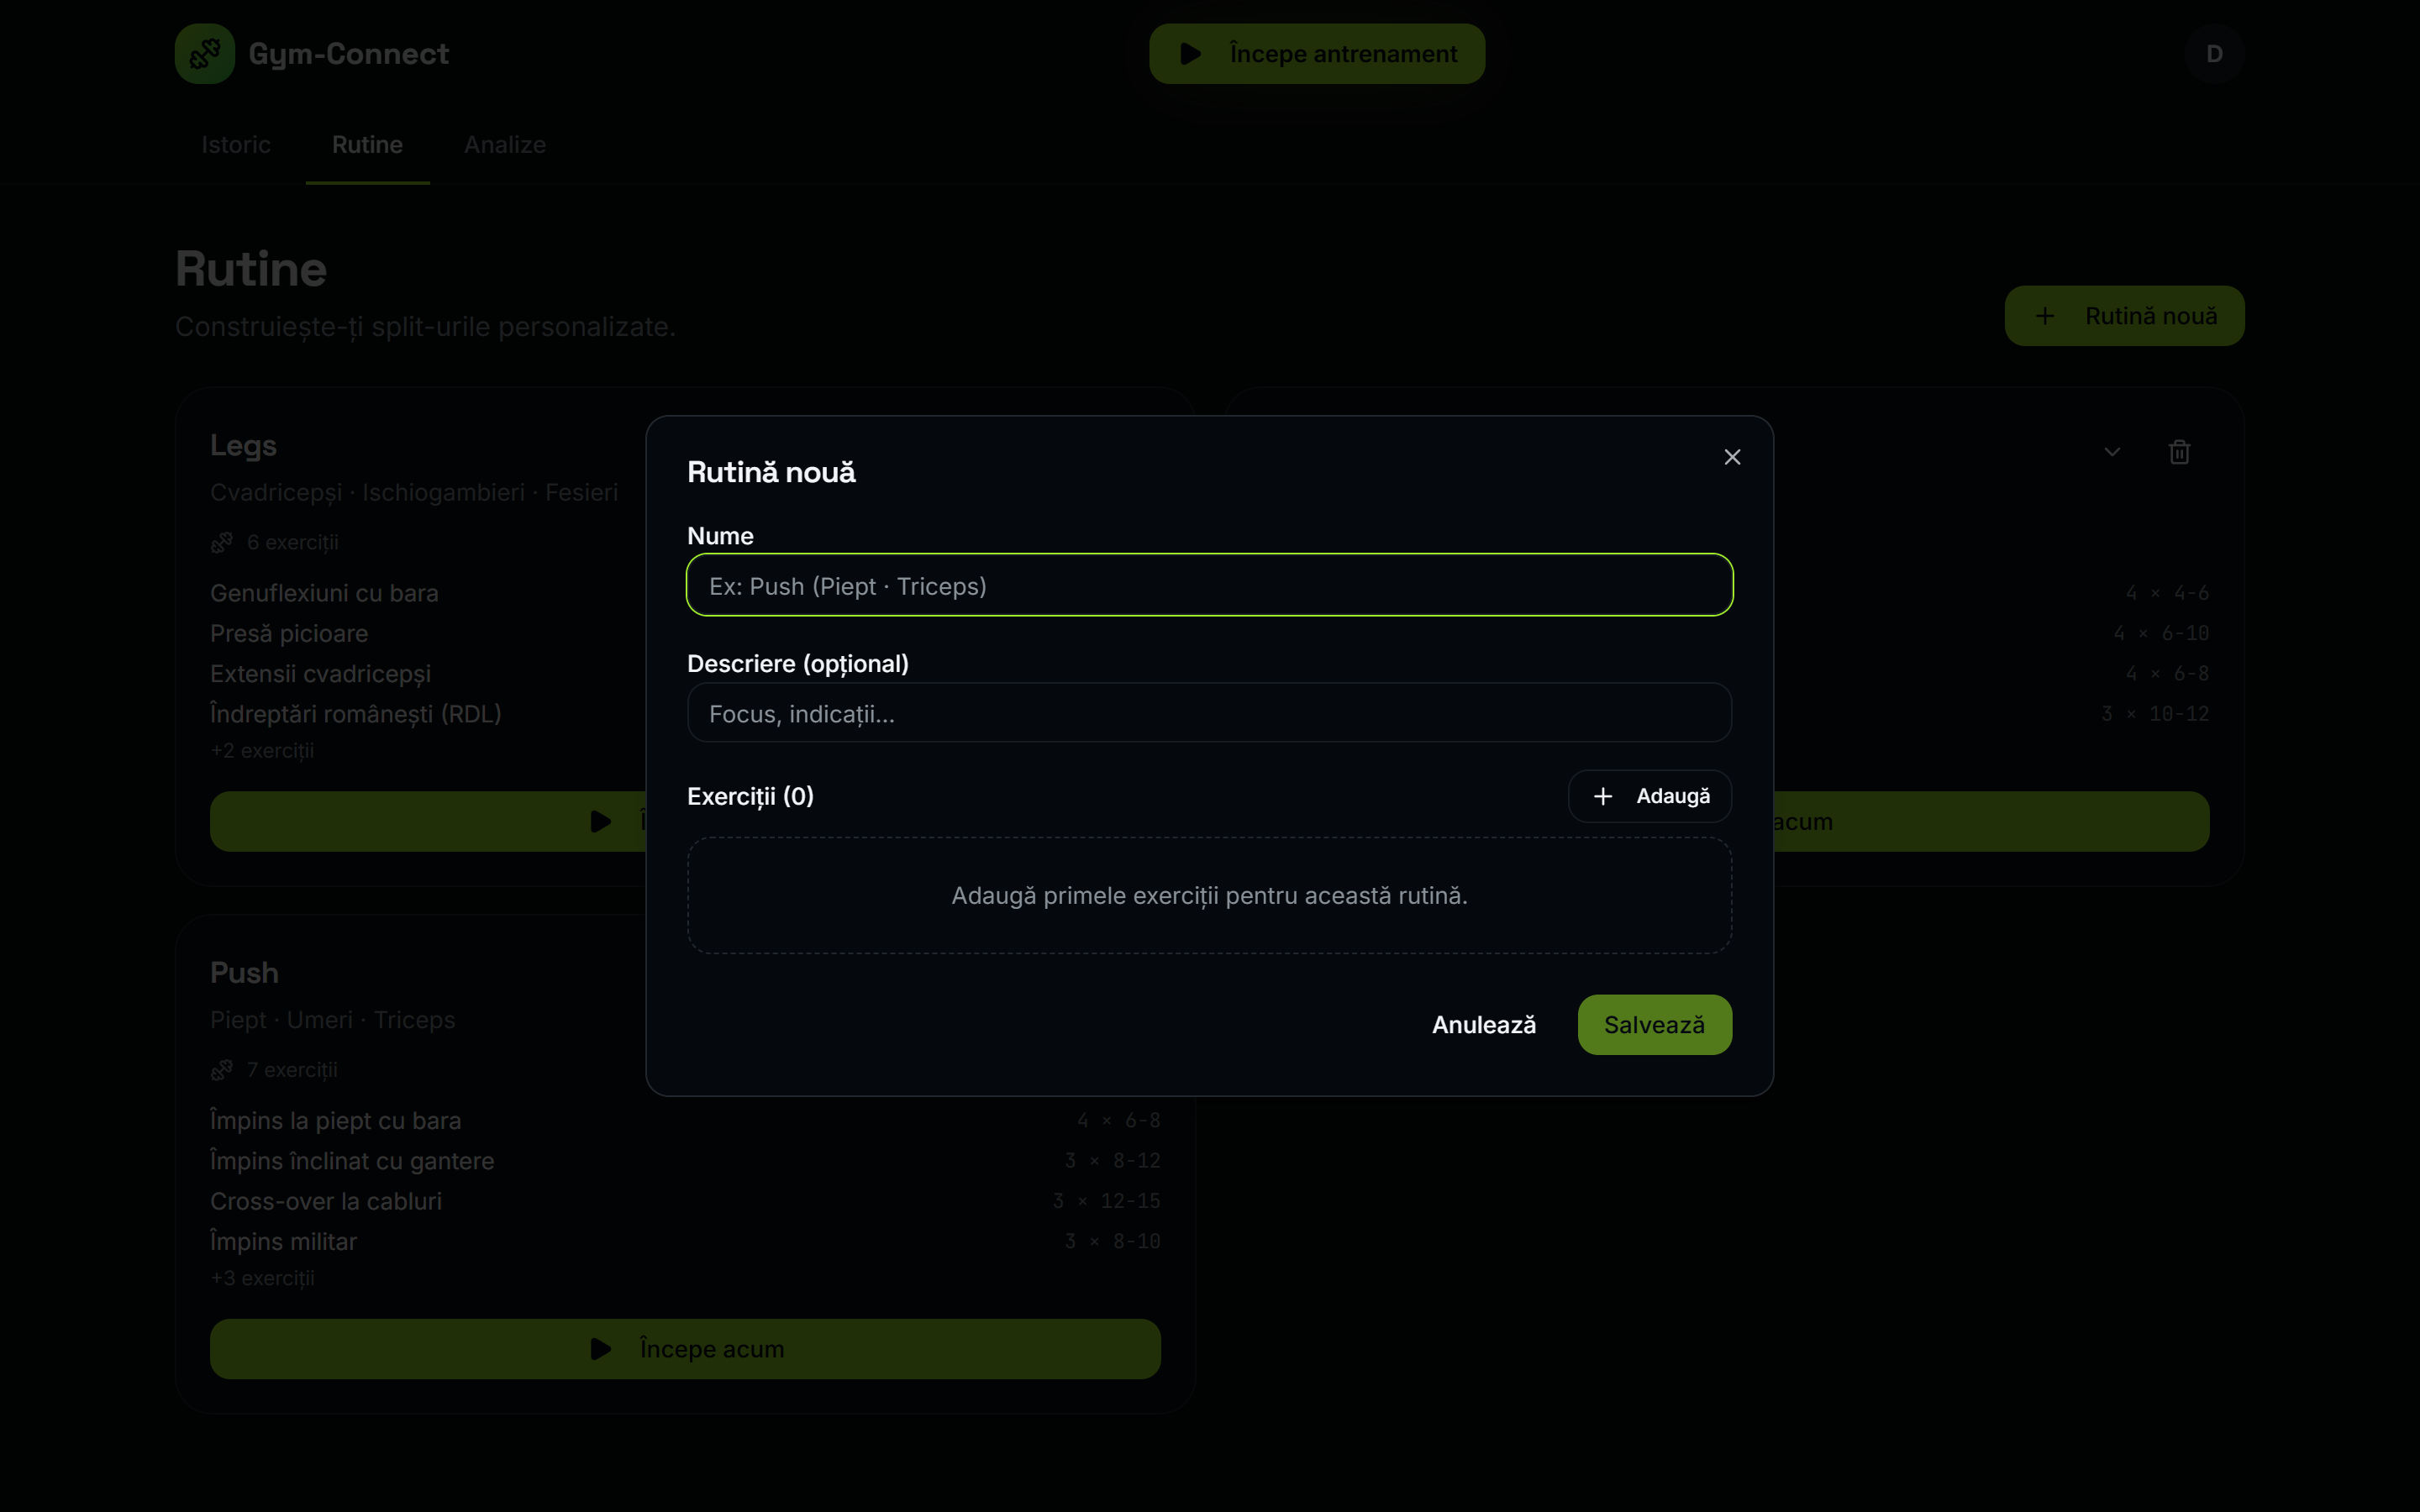
\includegraphics[width=\textwidth]{split-create.png}
  \caption{Crearea unei rutine}
  \label{fig:split-create}
\end{figure}

\subsection{Selectorul de exerci\c tii}

Ad\u augarea exerci\c tiilor se face printr-un selector
(figura~\ref{fig:exercise-picker}) care afi\c seaz\u a biblioteca de exerci\c tii
grupat\u a pe grupe musculare. Utilizatorul poate c\u auta rapid un exerci\c tiu
dup\u a nume \c si \^ il adaug\u a \^ in rutin\u a cu un singur click.

\begin{figure}[H]
  \centering
  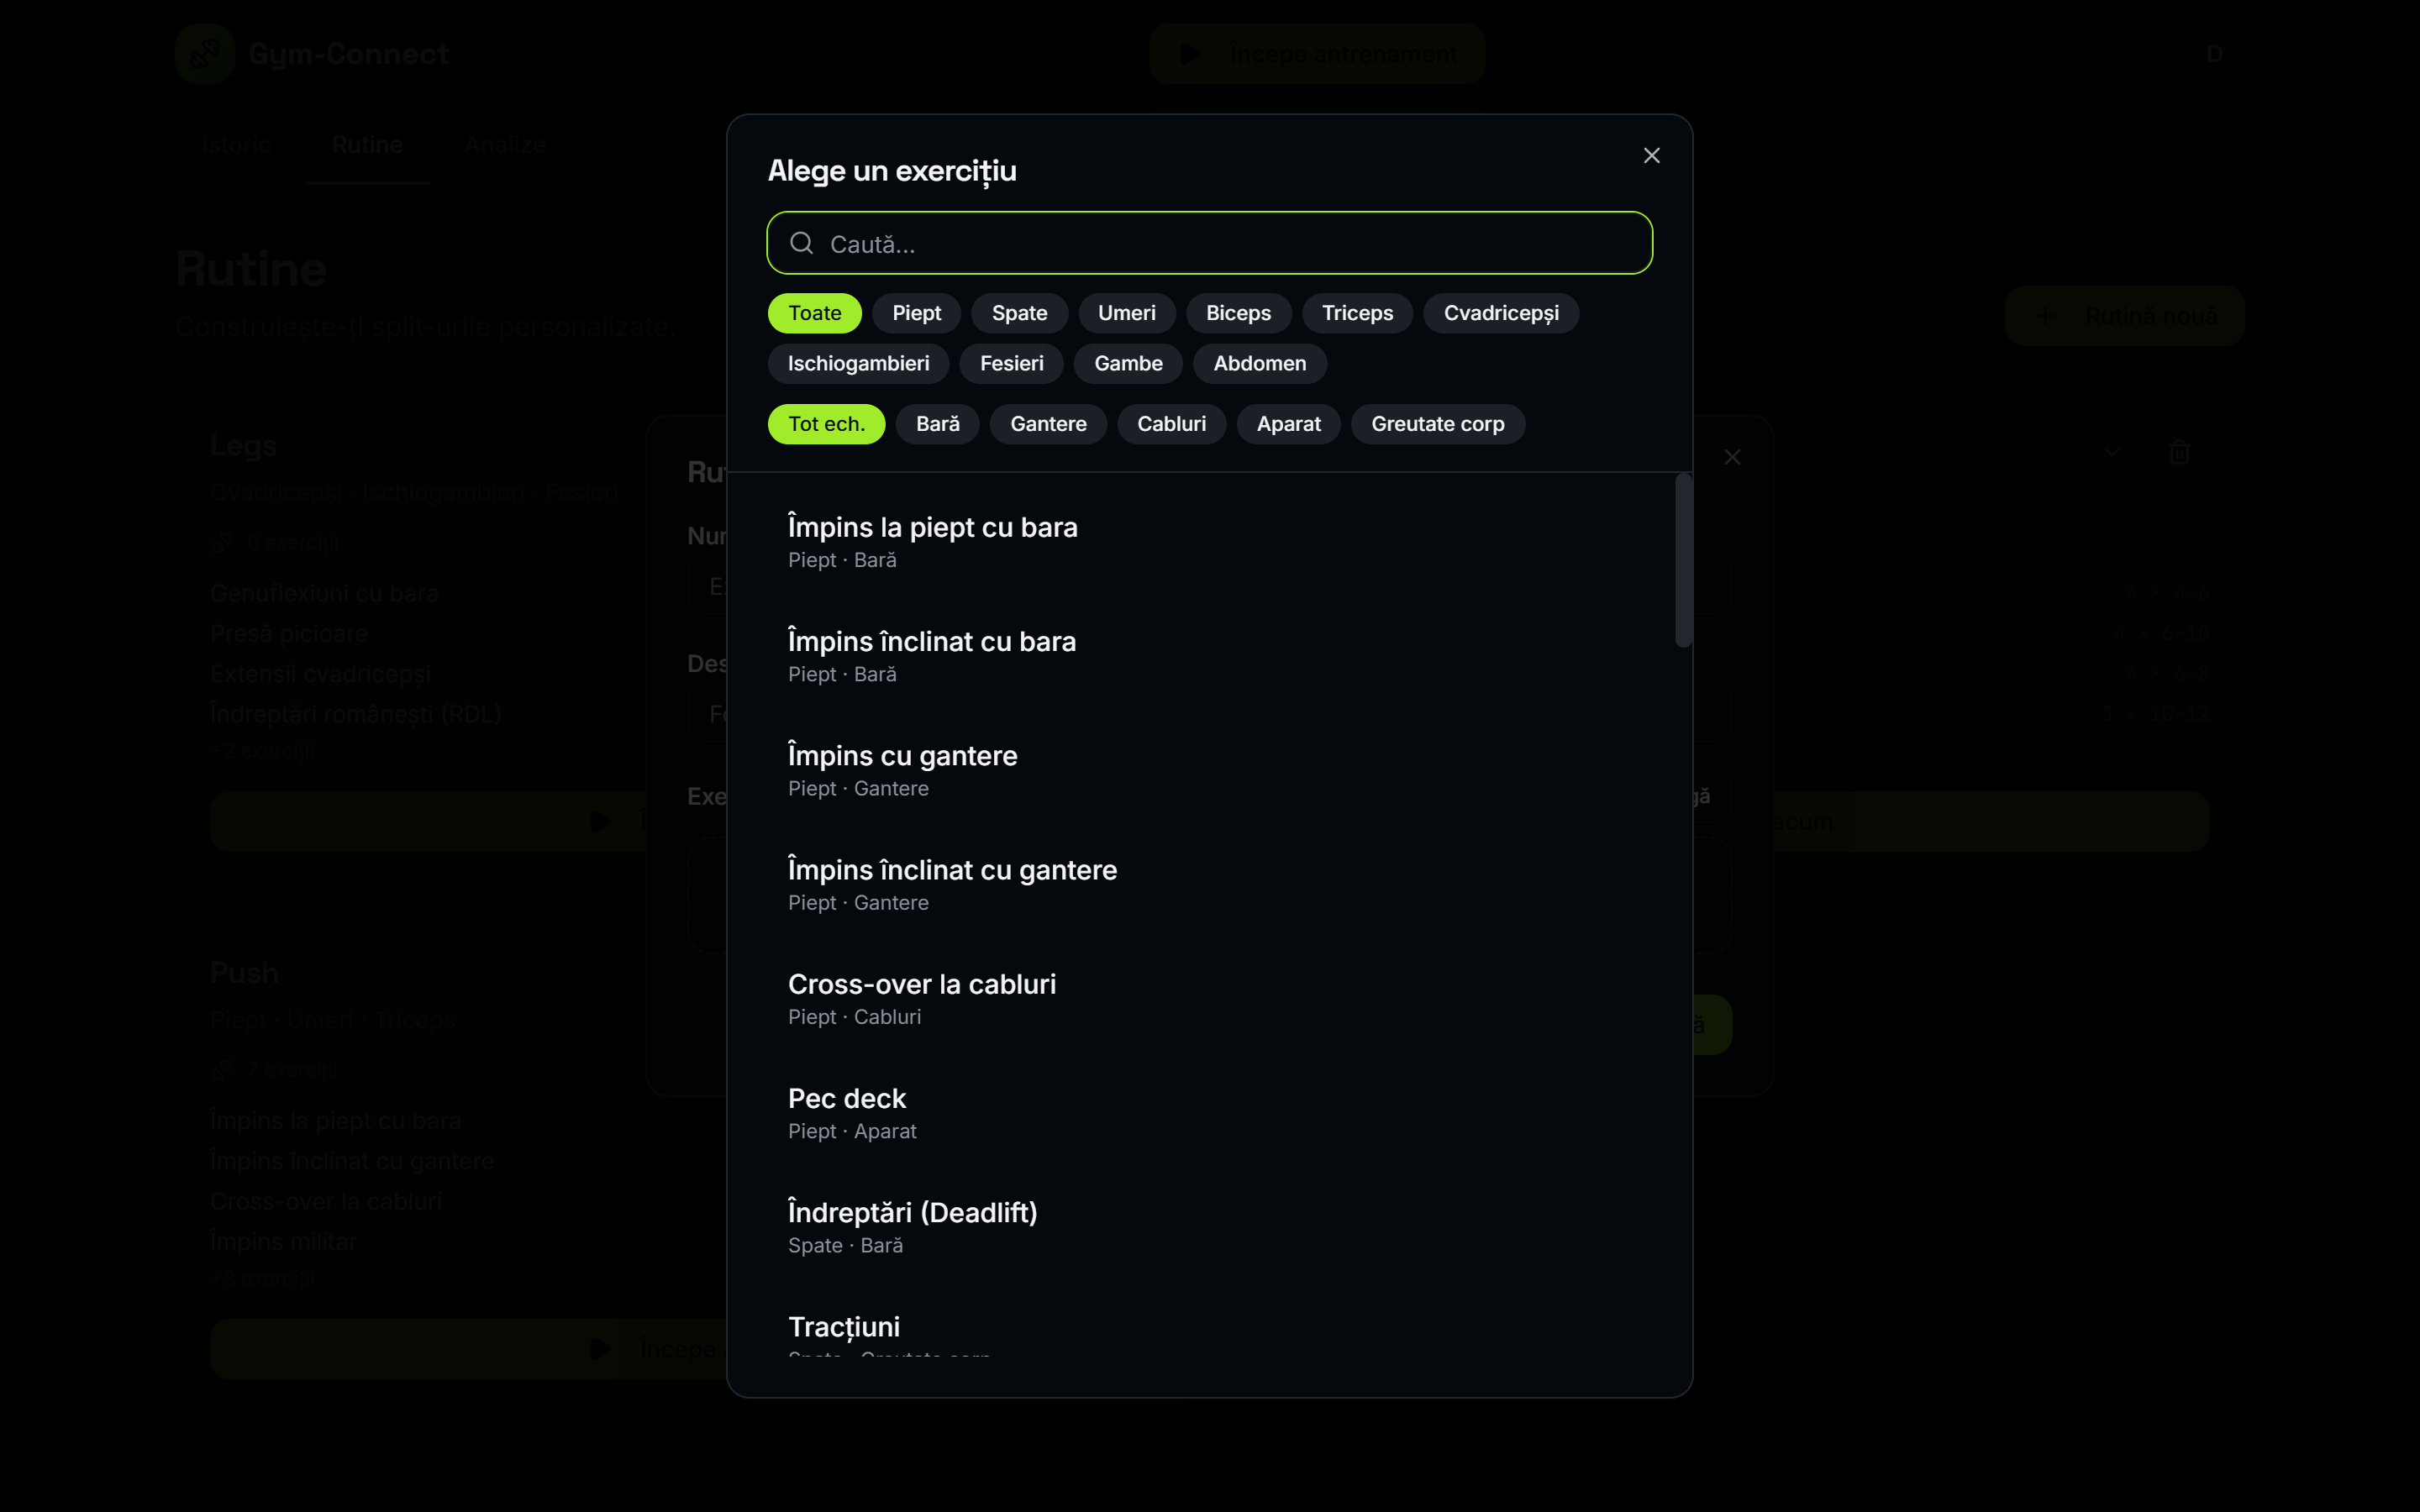
\includegraphics[width=\textwidth]{exercise-picker.png}
  \caption{Selectorul de exerci\c tii}
  \label{fig:exercise-picker}
\end{figure}

\section{Sesiunea de antrenament (Workout)}

Modulul de antrenament (figura~\ref{fig:workout}) este inima aplica\c tiei --
ecranul pe care utilizatorul \^ il folose\c ste efectiv \^ in sal\u a. Aici se
desf\u a\c soar\u a sesiunea \^ in timp real: exerci\c tiile din rutin\u a sunt
afi\c sate pe r\^ and, iar seturile se completeaz\u a pe m\u asur\u a ce sunt
efectuate.

\begin{figure}[H]
  \centering
  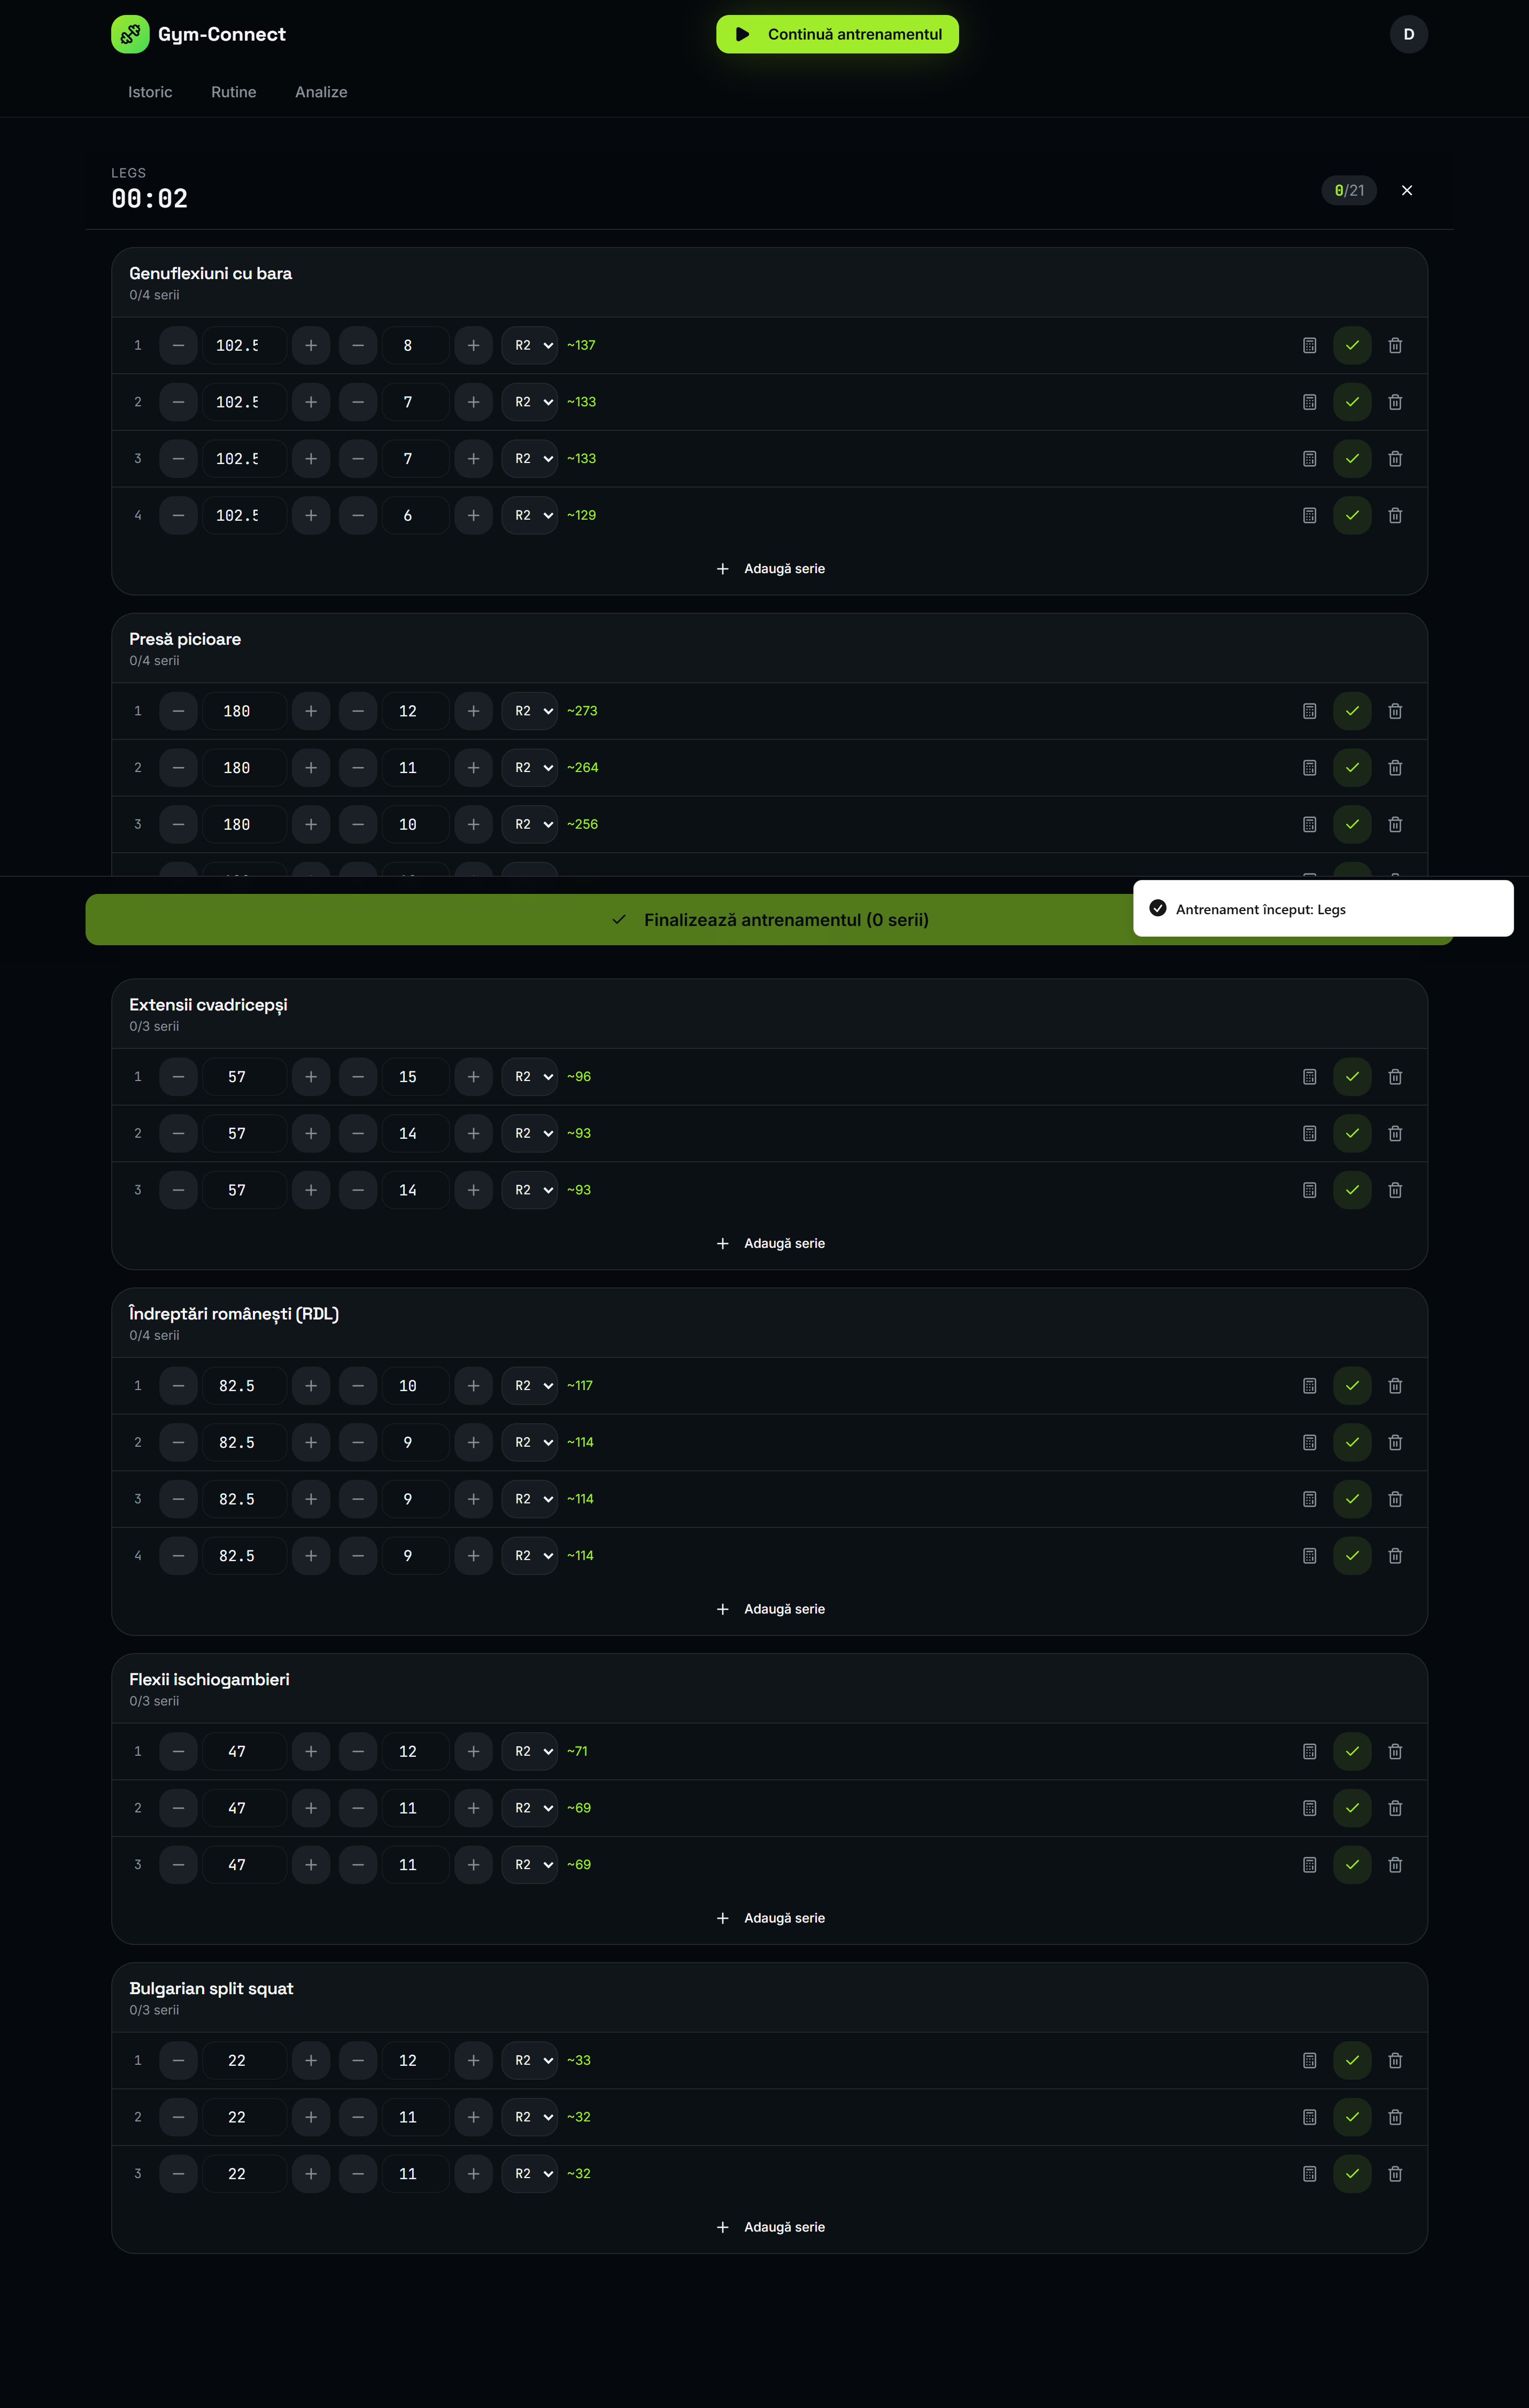
\includegraphics[height=0.78\textheight]{workout.png}
  \caption{Sesiunea de antrenament}
  \label{fig:workout}
\end{figure}

\subsection{Cronometrul \c si indicatorul de progres}

Dup\u a fiecare set, aplica\c tia porne\c ste automat un cronometru de odihn\u a
(figura~\ref{fig:timer}), \^ inso\c tit de un indicator care arat\u a c\^ ate
seturi au fost finalizate din totalul planificat. Acest detaliu m\u arunt
conteaz\u a \^ in practic\u a: nu mai trebuie s\u a urm\u are\c sti pauza separat,
pe telefon.

\begin{figure}[H]
  \centering
  
\includegraphics[width=\textwidth]{timer.png}
  \caption{Cronometrul \c si indicatorul de progres}
  \label{fig:timer}
\end{figure}

\subsection{Gestionarea seturilor}

\^ Inregistrarea propriu-zis\u a a seturilor este prezentat\u a \^ in
figura~\ref{fig:sets}. Pentru fiecare exerci\c tiu, utilizatorul introduce
greutatea \c si num\u arul de repeti\c tii, fiecare set ap\u ar\^ and pe un r\^ and
separat, u\c sor de urm\u arit.

\begin{figure}[H]
  \centering
  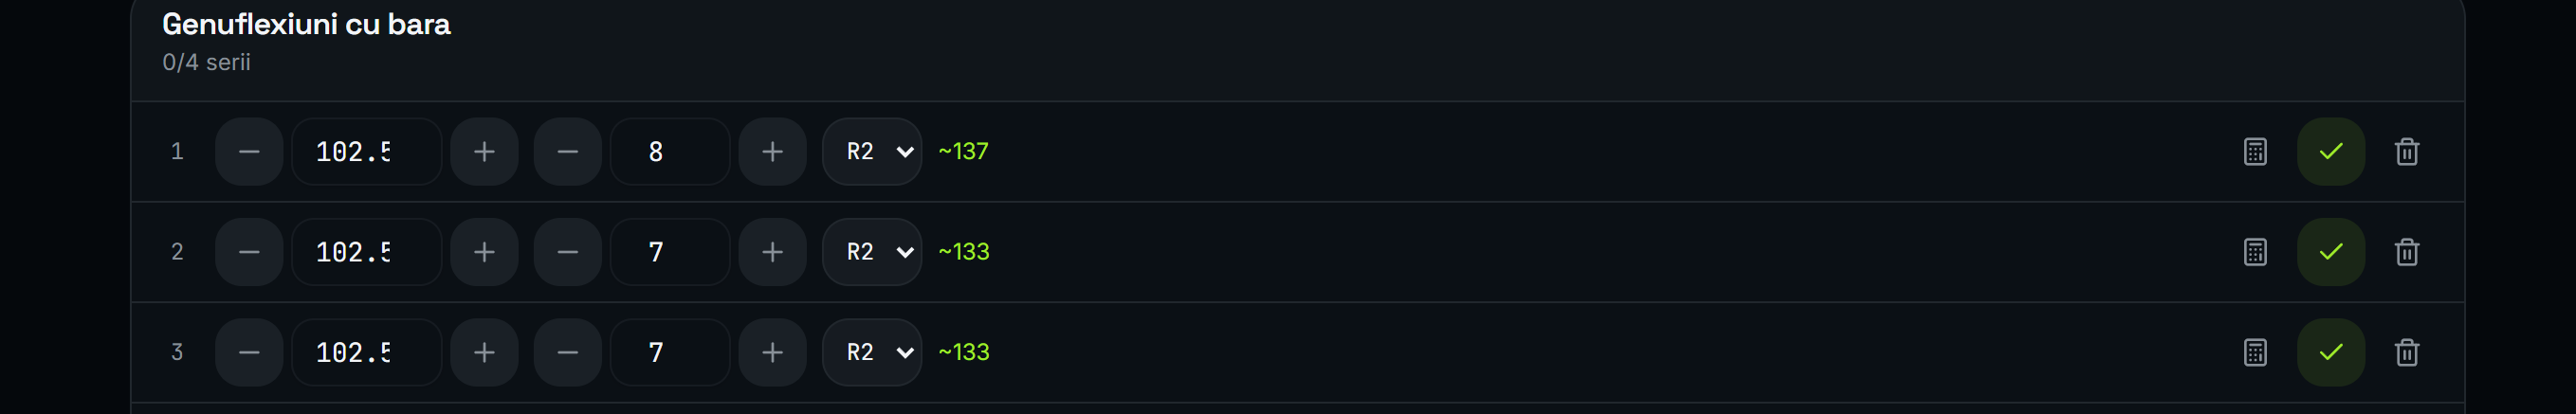
\includegraphics[width=\textwidth]{sets.png}
  \caption{Gestionarea seturilor}
  \label{fig:sets}
\end{figure}

\subsection{Calculatorul de pl\u aci}

Un instrument pe care \^ il consider deosebit de util este calculatorul de
pl\u aci (figura~\ref{fig:plates}). Pornind de la greutatea \c tint\u a, acesta
calculeaz\u a exact ce discuri trebuie puse pe fiecare cap\u at al barei de
20~kg, sc\u ap\^ andu-l pe utilizator de un calcul mental incomod \^ in mijlocul
antrenamentului.

\begin{figure}[H]
  \centering
  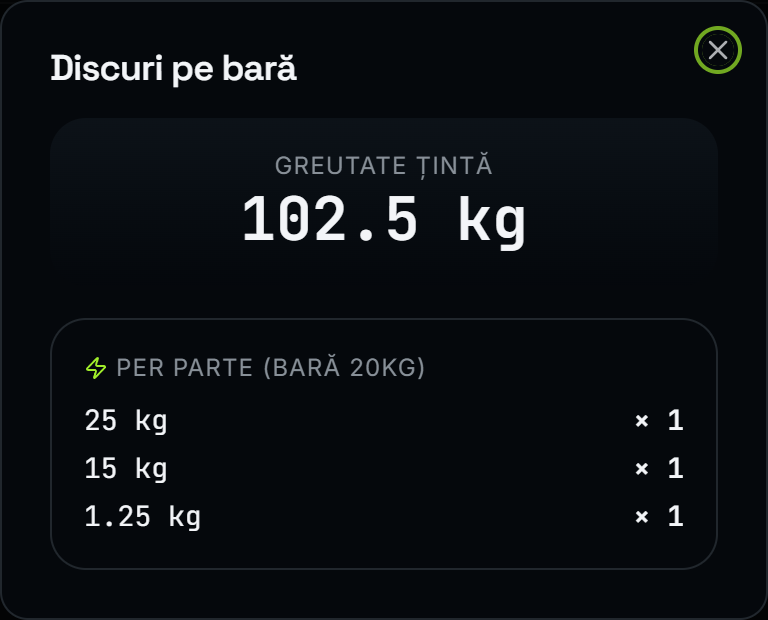
\includegraphics[width=0.5\textwidth]{plates.png}
  \caption{Calculatorul de pl\u aci}
  \label{fig:plates}
\end{figure}

\subsection{Indicatori de intensitate: RIR \c si 1RM}

Figura~\ref{fig:intensity} arat\u a cum aplica\c tia capteaz\u a intensitatea
efortului. Pe l\^ ang\u a greutate \c si repeti\c tii, fiecare set are asociat\u a
o valoare RIR (\textit{Reps in Reserve}), iar aplica\c tia calculeaz\u a \c si
afi\c seaz\u a imediat 1RM-ul estimat pentru setul respectiv.

\begin{figure}[H]
  \centering
  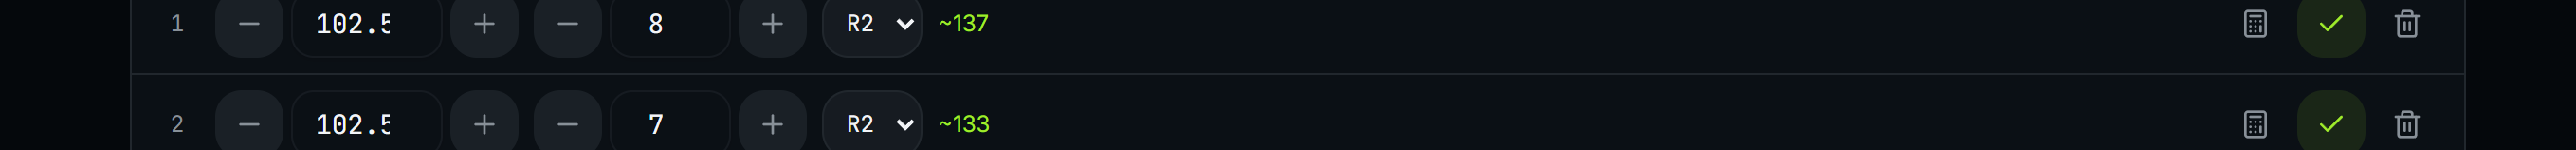
\includegraphics[width=\textwidth]{intensity.png}
  \caption{Indicatori de intensitate: RIR \c si 1RM}
  \label{fig:intensity}
\end{figure}

\section{Istoricul antrenamentelor (History)}

Istoricul antrenamentelor (figura~\ref{fig:history}) func\c tioneaz\u a ca un
jurnal: toate sesiunile anterioare sunt listate cronologic, \^ impreun\u a cu
statistici de ansamblu precum volumul total ridicat \c si durata medie a unui
antrenament. De aici utilizatorul \^ i\c si poate urm\u ari activitatea pe termen
lung.

\begin{figure}[H]
  \centering
  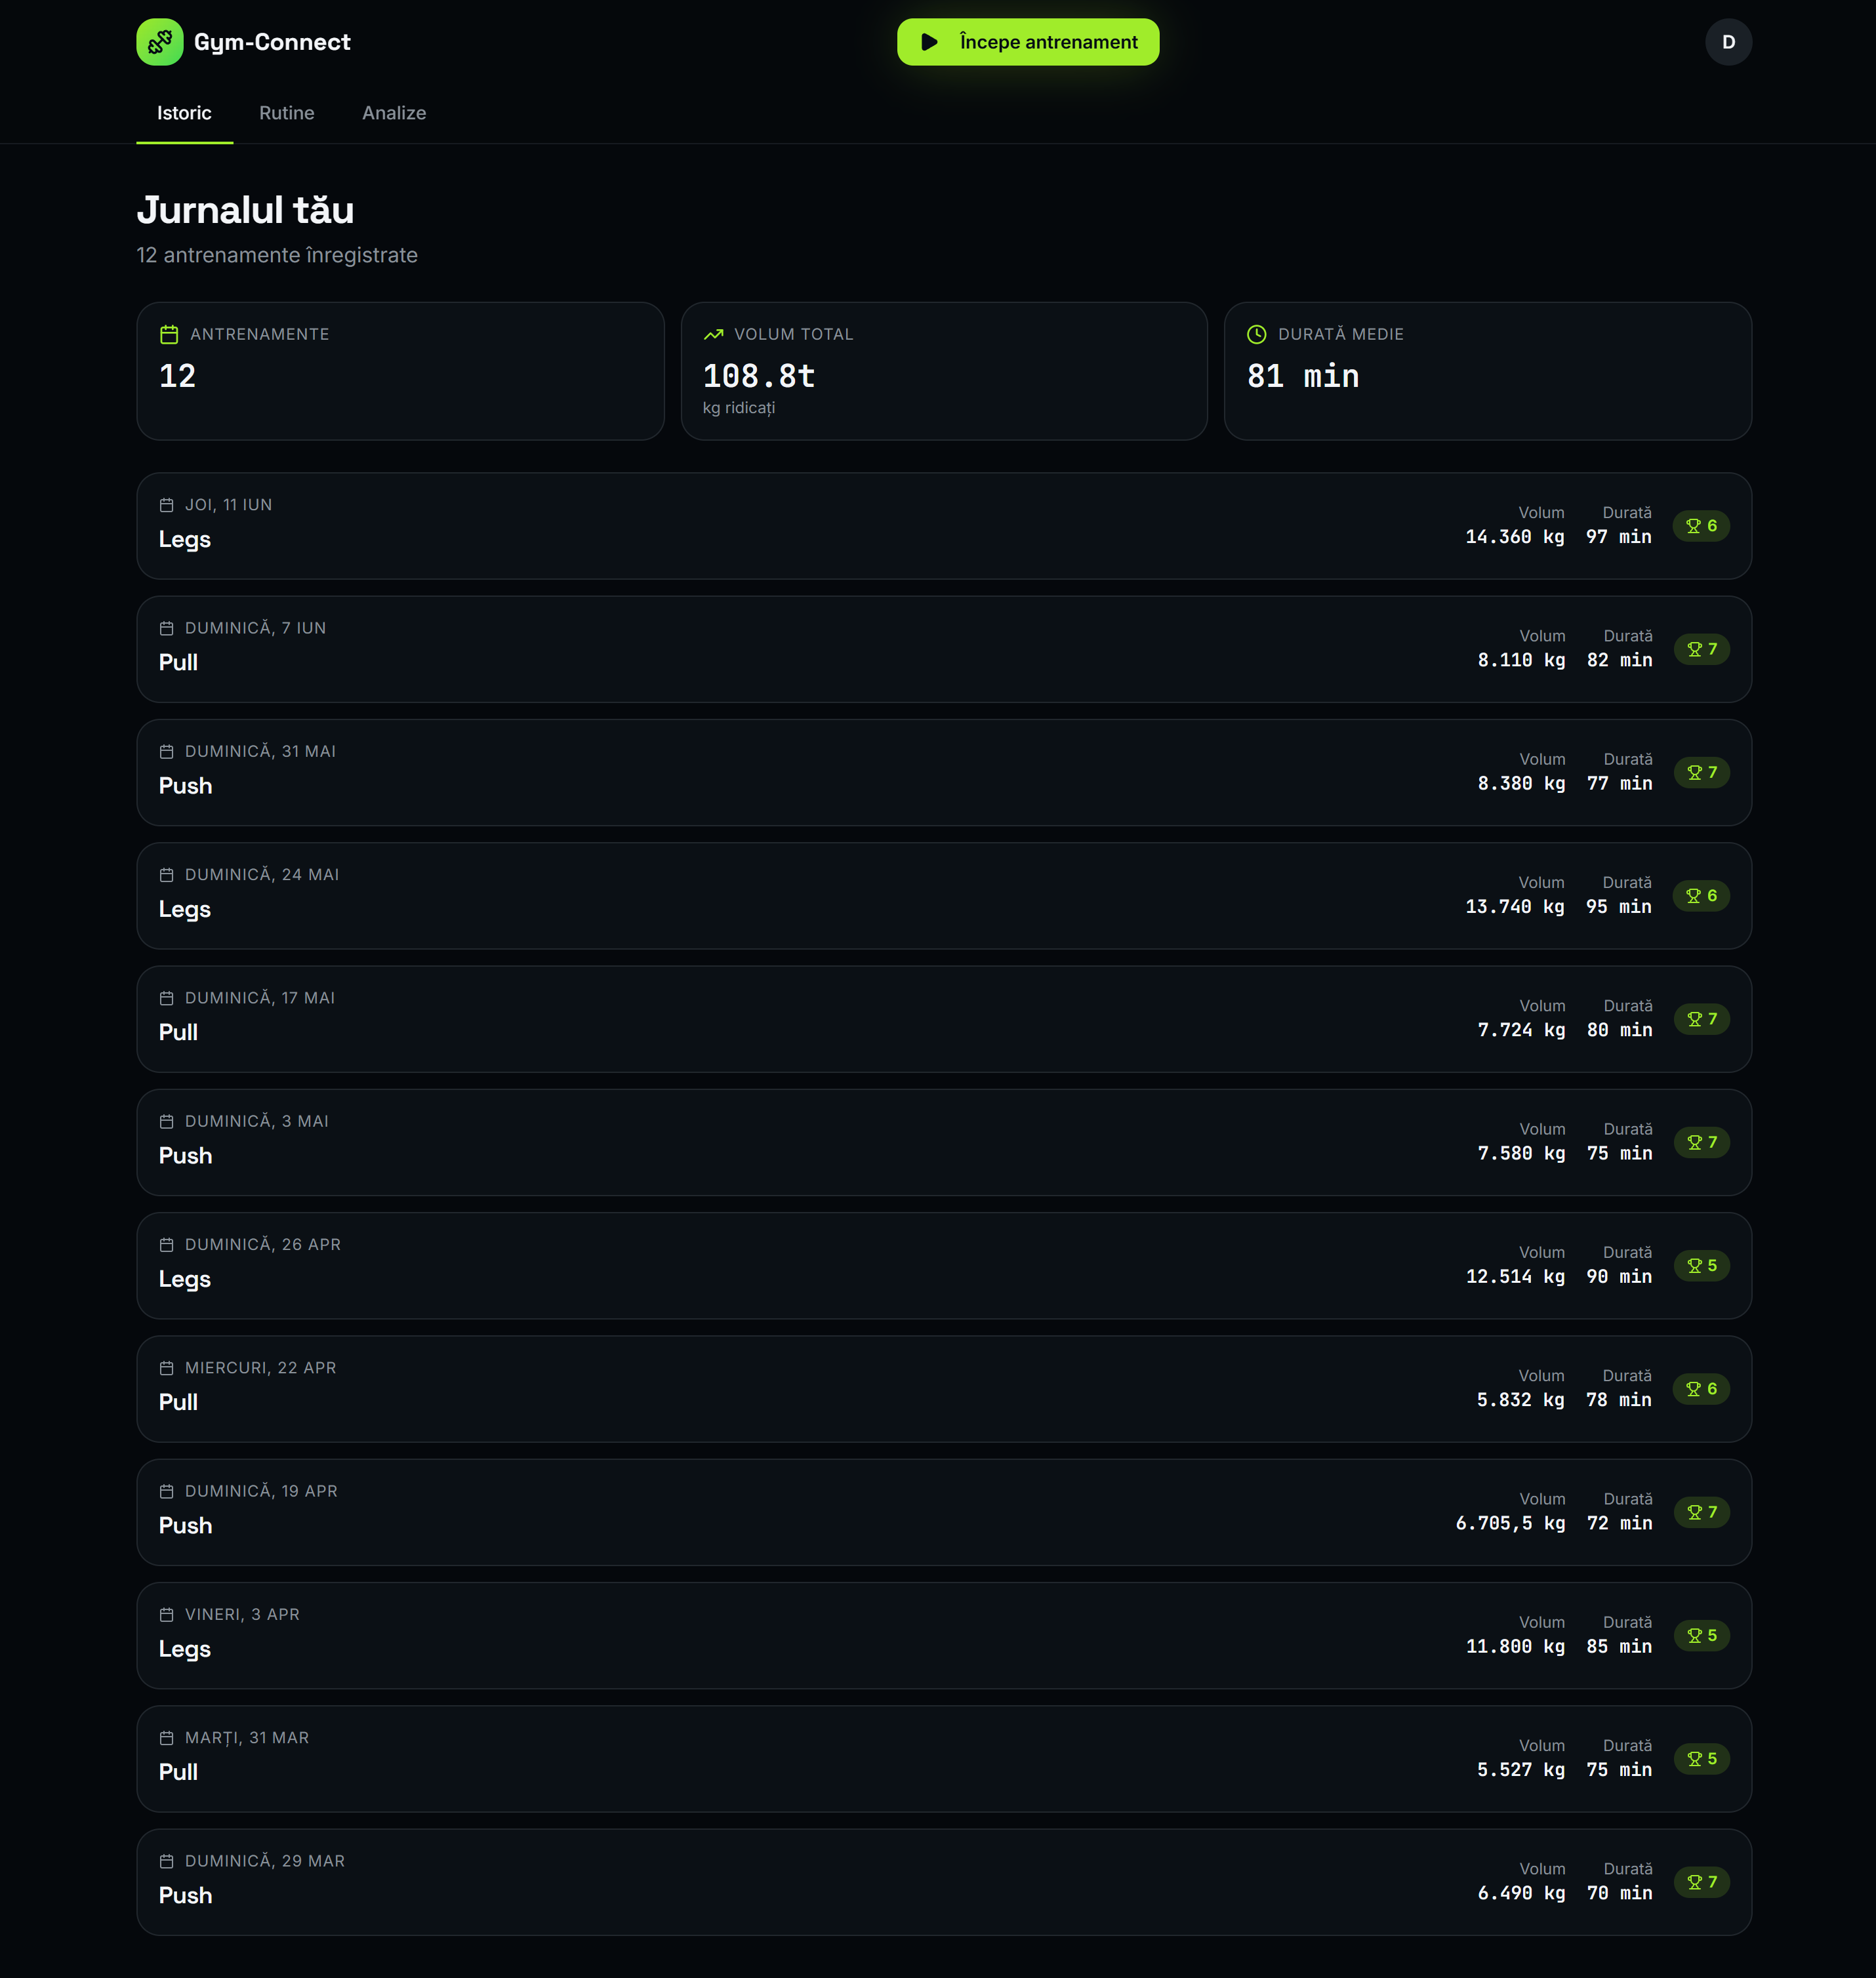
\includegraphics[width=0.8\textwidth]{history.png}
  \caption{Istoricul antrenamentelor}
  \label{fig:history}
\end{figure}

\section{Modulul de analitic\u a (Analytics)}

Modulul de analitic\u a (figura~\ref{fig:analytics}) este, \^ in opinia mea,
partea cea mai valoroas\u a a aplica\c tiei. El transform\u a datele brute din
istoric \^ in informa\c tie util\u a, prin dou\u a grafice principale \c si un
sistem de avertizare, pe care le detaliez \^ in continuare.

\begin{figure}[H]
  \centering
  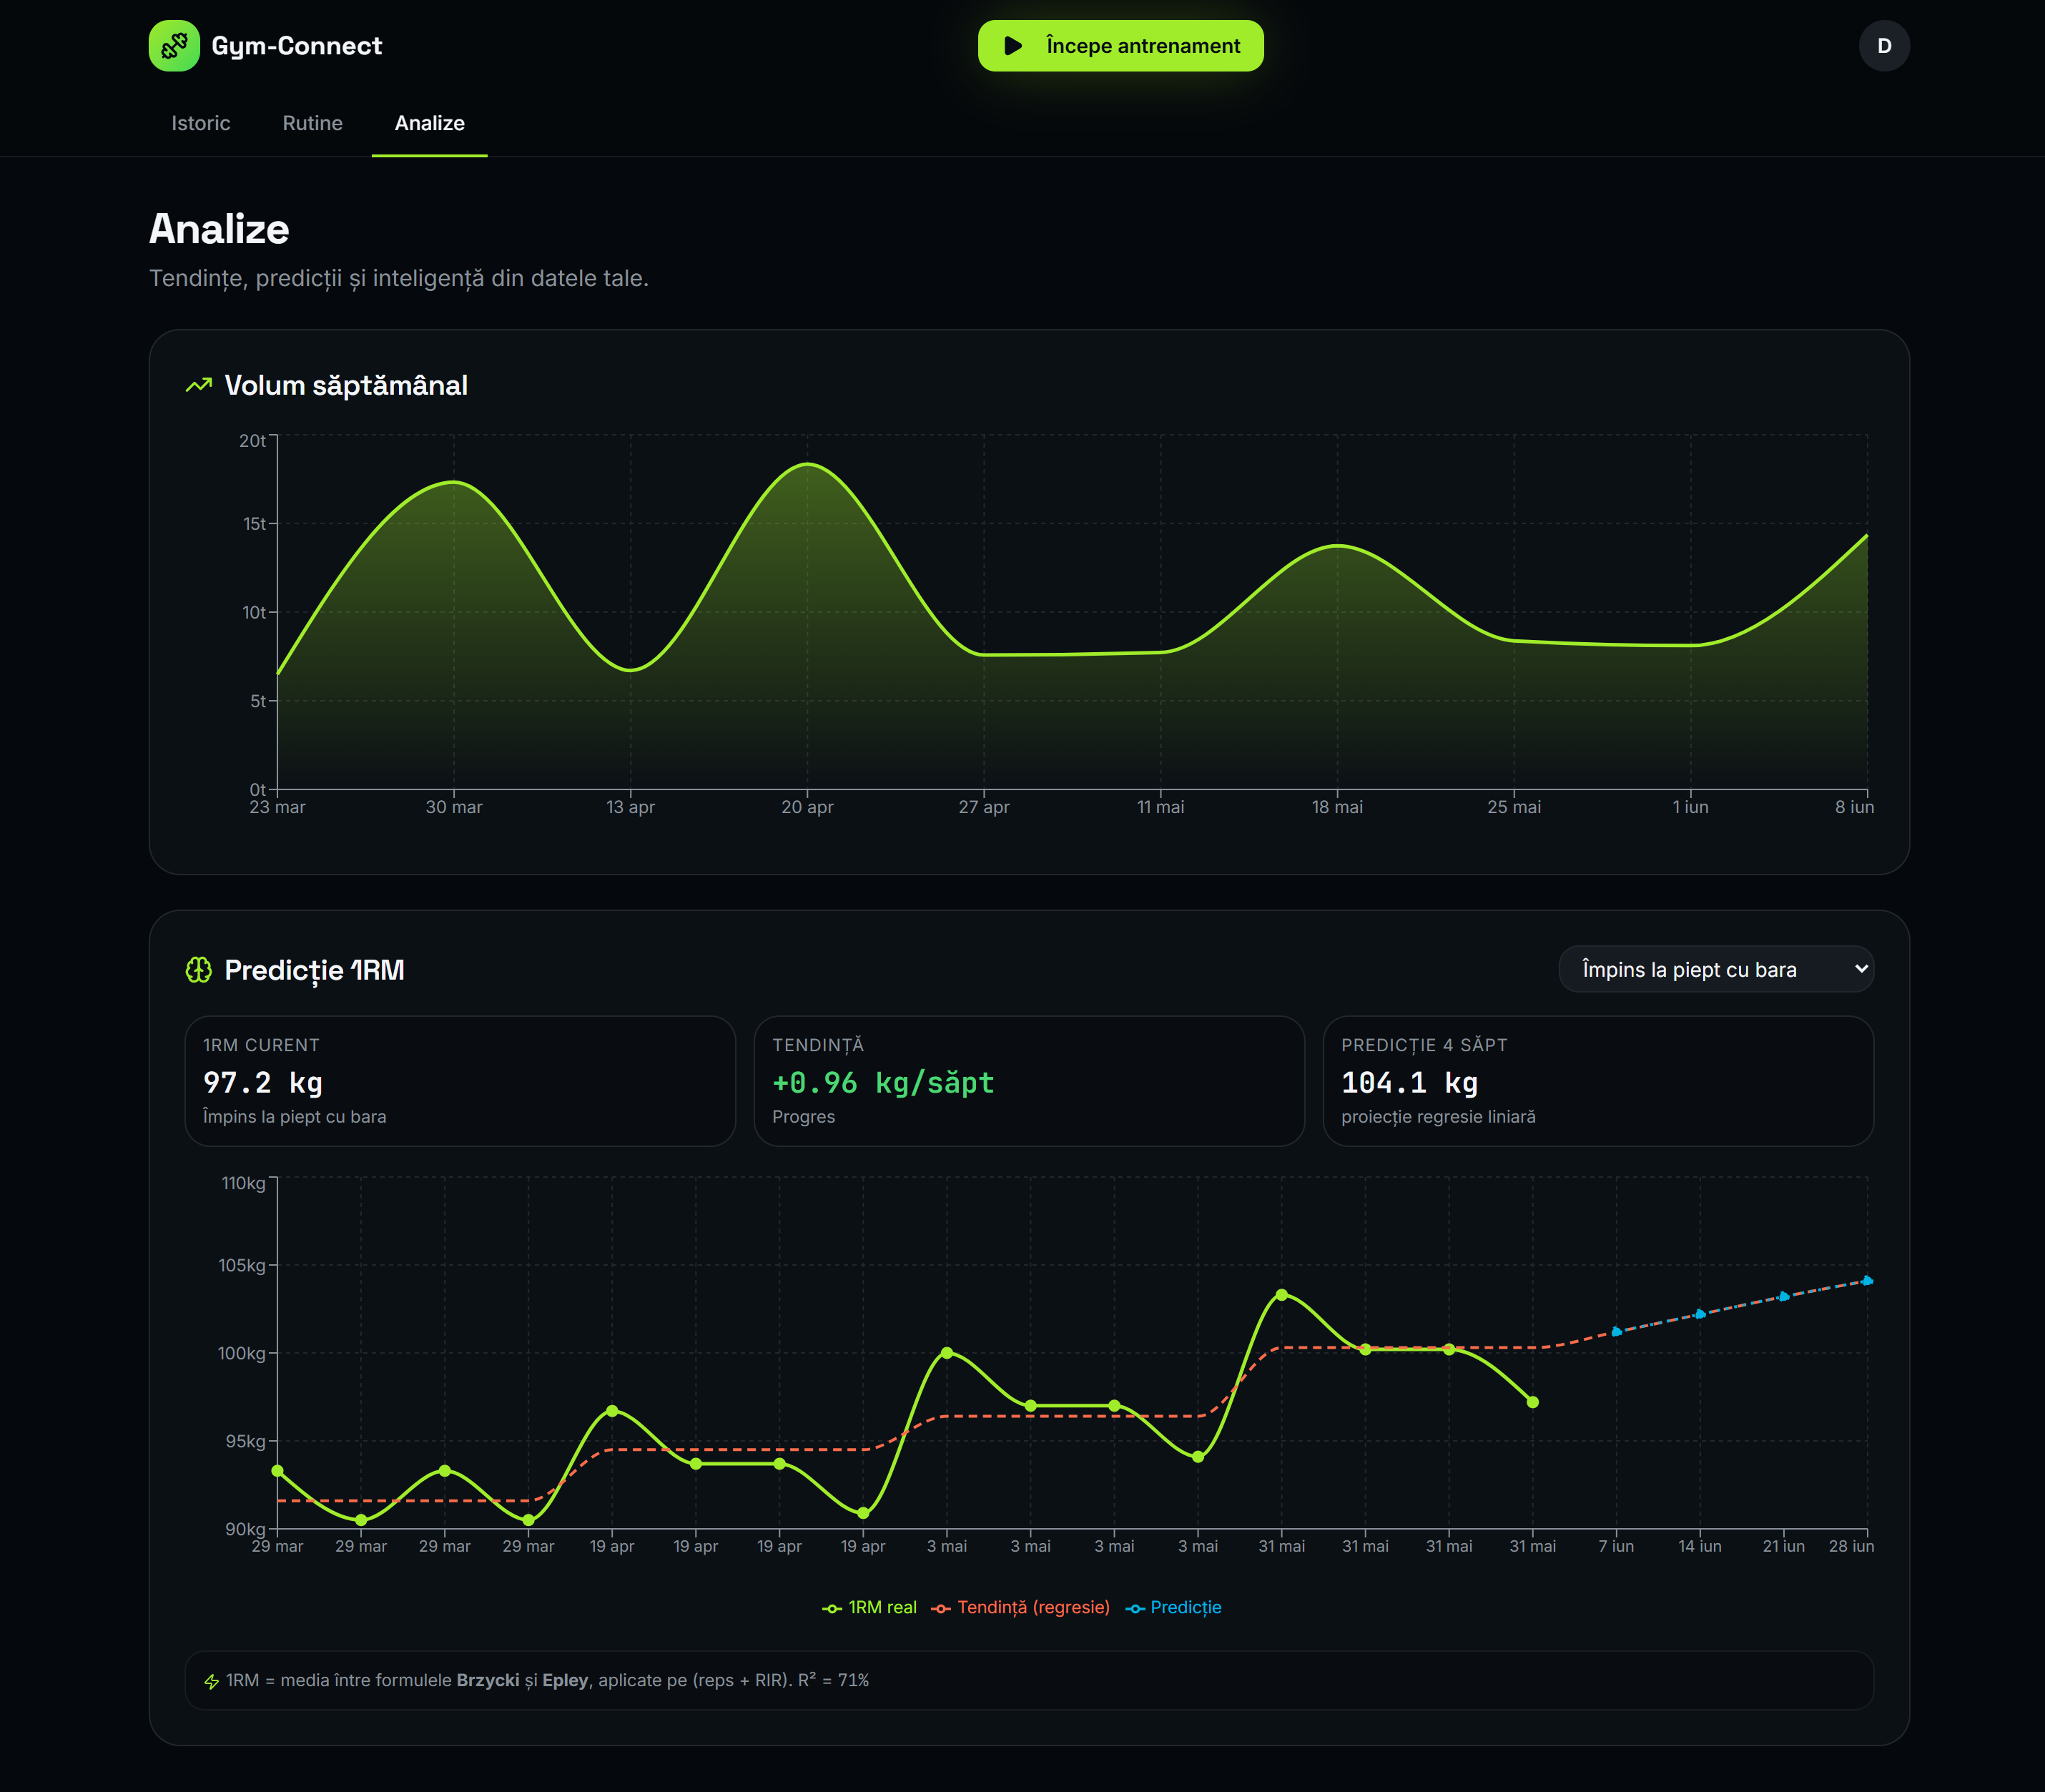
\includegraphics[width=\textwidth]{analytics.png}
  \caption{Modulul de analitic\u a}
  \label{fig:analytics}
\end{figure}

\subsection{Graficul volumului s\u apt\u am\^ anal}

Primul grafic (figura~\ref{fig:volume}) prezint\u a volumul total de
antrenament, agregat pe s\u apt\u am\^ ani. Vizualizarea ajut\u a utilizatorul
s\u a \^ in\c teleag\u a dac\u a \^ i\c si cre\c ste treptat \^ inc\u arc\u atura --
esen\c ta principiului \textit{progressive overload}.

\begin{figure}[H]
  \centering
  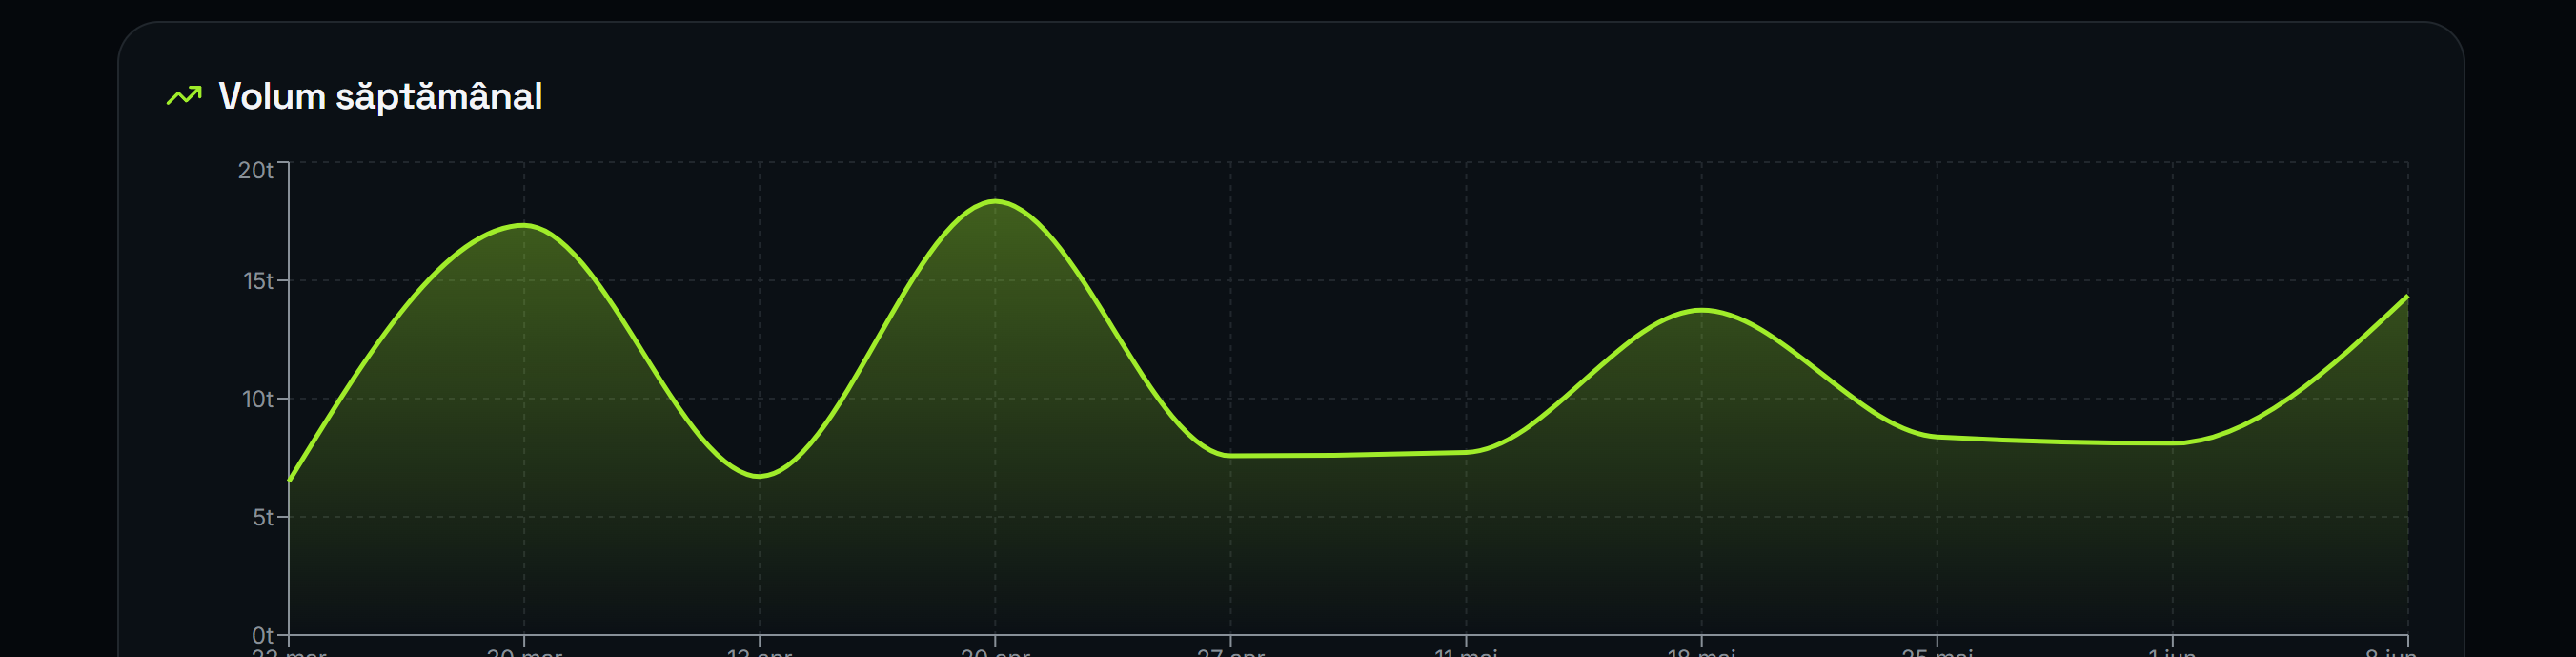
\includegraphics[width=\textwidth]{volume.png}
  \caption{Graficul volumului s\u apt\u am\^ anal}
  \label{fig:volume}
\end{figure}

\subsection{Predic\c tia 1RM \c si regresia liniar\u a}

Al doilea grafic (figura~\ref{fig:prediction}) aplic\u a regresia liniar\u a
peste valorile 1RM estimate de-a lungul timpului. Linia continu\u a reprezint\u a
valorile reale, cea punctat\u a tendin\c ta calculat\u a, iar por\c tiunea
final\u a proiecteaz\u a evolu\c tia probabil\u a pe urm\u atoarele patru
s\u apt\u am\^ ani.

\begin{figure}[H]
  \centering
  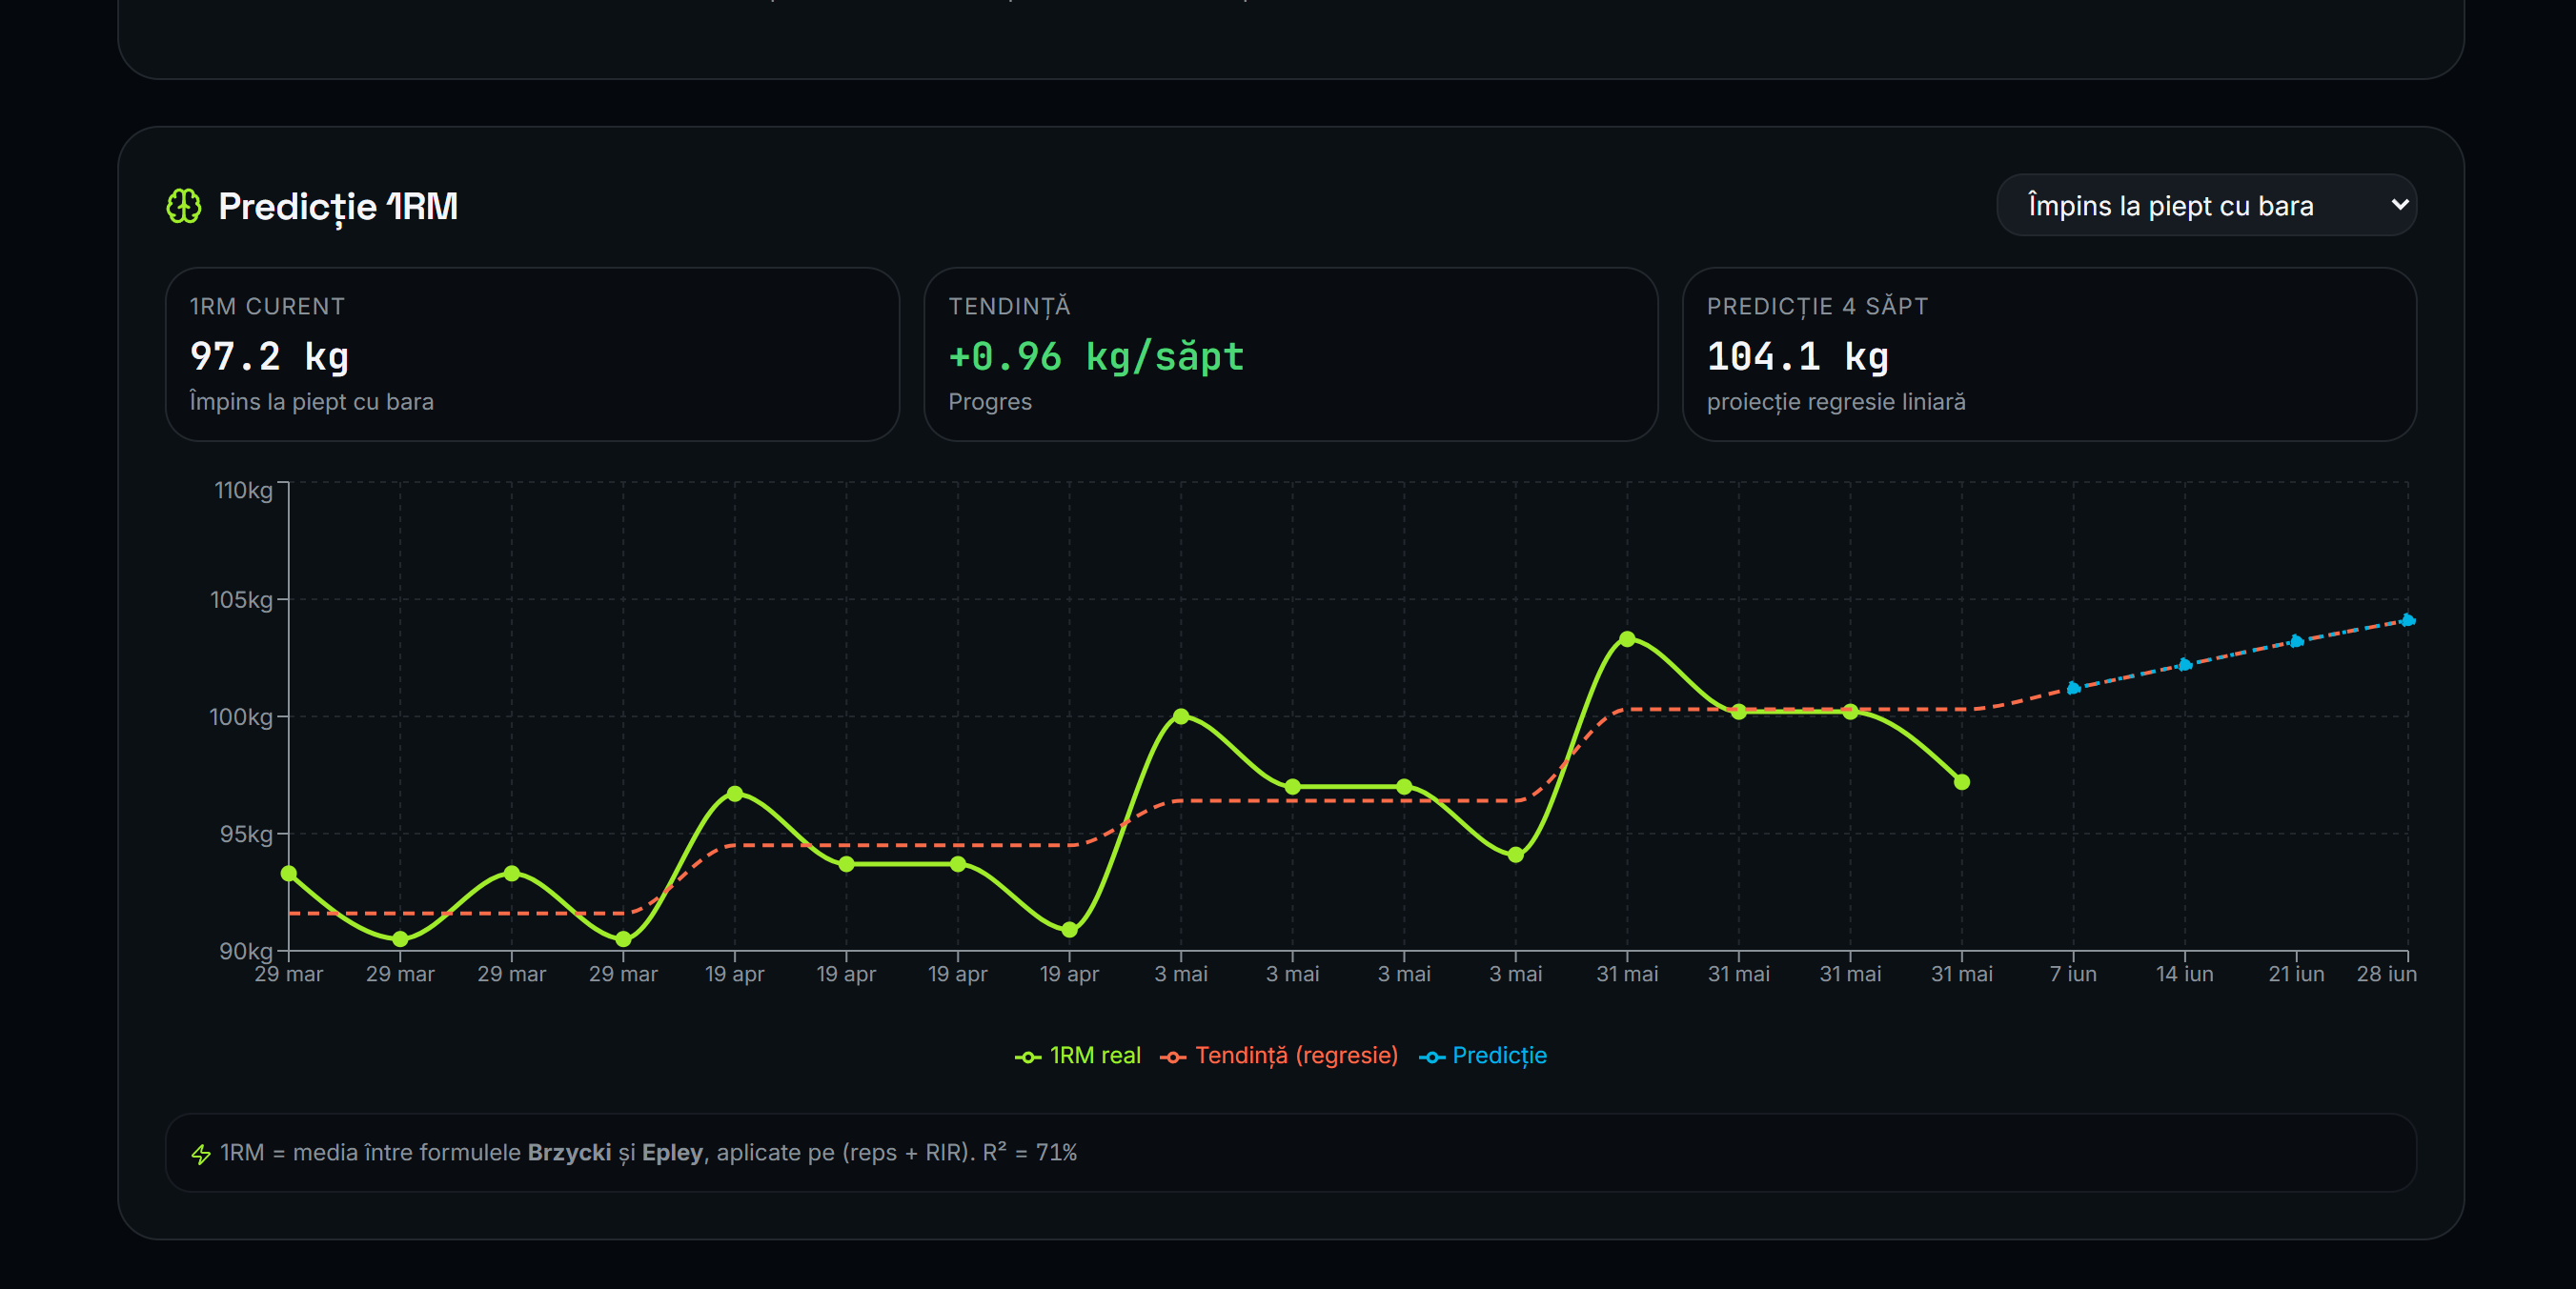
\includegraphics[width=\textwidth]{prediction.png}
  \caption{Predic\c tia 1RM \c si regresia liniar\u a}
  \label{fig:prediction}
\end{figure}

\subsection{Detec\c tia platourilor}

Atunci c\^ and volumul s\u apt\u am\^ anal scade cu peste 5\% pe parcursul a trei
s\u apt\u am\^ ani, aplica\c tia afi\c seaz\u a automat un avertisment de platou
(figura~\ref{fig:plateau}), suger\^ and utilizatorului c\u a ar putea avea
nevoie de o s\u apt\u am\^ an\u a de \textit{deload}. Astfel, stagnarea este
semnalat\u a \^ inainte s\u a devin\u a o problem\u a.

\begin{figure}[H]
  \centering
  
\includegraphics[width=\textwidth]{plateau.png}
  \caption{Detec\c tia platourilor}
  \label{fig:plateau}
\end{figure}
 % Cap. 5 - Prezentarea aplicatiei
\chapter{Concluzii}

\section{Rezultate ob\c tinute}

La finalul acestui proiect pot spune c\u a obiectivul principal a fost
atins: Gym-Connect este o aplica\c tie web func\c tional\u a, care
rezolv\u a exact problema de la care am pornit -- gestionarea ordonat\u a
a antrenamentelor de for\c t\u a \c si urm\u arirea progresului pe termen
lung, totul gratuit \c si accesibil direct din browser.

Concret, aplica\c tia implementeaz\u a toate func\c tionalit\u a\c tile
propuse \^ in capitolul introductiv. Utilizatorul \^ i\c si poate crea
cont \c si autentifica \^ in siguran\c t\u a prin Clerk, \^ i\c si poate
defini rutine de antrenament personalizate cu exerci\c tii, seturi \c si
intervale de repeti\c tii \c tint\u a, \c si poate \^ inregistra sesiuni
de antrenament \^ in timp real. Modulul de antrenament ofer\u a un timer
de odihn\u a \^ intre seturi, un calculator de distribu\c tie a pl\u acilor
pe bar\u a \c si suport pentru indicatorii de intensitate RIR \c si 1RM
estimat. \^ In plus, toate datele introduse de un utilizator sunt
izolate complet de ale celorlal\c ti, prin legarea fiec\u arei
\^ inregistr\u ari de identificatorul Clerk.

Cea mai valoroas\u a parte a aplica\c tiei r\u am\^ ane, \^ in opinia mea,
modulul de analitic\u a. Acesta nu doar afi\c seaz\u a un istoric brut
al antrenamentelor, ci transform\u a datele \^ in informa\c tie util\u a:
calculeaz\u a volumul s\u apt\u am\^ anal de antrenament, estimeaz\u a
evolu\c tia for\c tei prin 1RM \c si, folosind regresia liniar\u a,
proiecteaz\u a o tendin\c t\u a pe urm\u atoarele s\u apt\u am\^ ani.
Func\c tia de detec\c tie automat\u a a platourilor avertizeaz\u a
utilizatorul atunci c\^ and progresul stagneaz\u a, suger\^ and momentul
potrivit pentru un deload. Tocmai aceste func\c tionalit\u a\c ti --
absente din versiunile gratuite ale aplica\c tiilor concurente
analizate \^ in Capitolul 2 -- reprezint\u a contribu\c tia original\u a
principal\u a a acestei lucr\u ari.

Din punct de vedere tehnic, proiectul a confirmat c\u a o stiv\u a
modern\u a, omogen\u a TypeScript at\^ at pe frontend c\^ at \c si pe
backend, permite dezvoltarea rapid\u a a unei aplica\c tii complete,
cu un cod u\c sor de \^ intre\c tinut \c si extins.

\section{Limit\u arile solu\c tiei actuale}

De\c si aplica\c tia \^ i\c si \^ indepline\c ste scopul, sunt con\c stient
de o serie de limit\u ari pe care le-am identificat pe parcurs.

\^ In primul r\^ and, predic\c tia evolu\c tiei 1RM se bazeaz\u a pe
regresie liniar\u a, un model simplu care presupune o cre\c stere
constant\u a \^ in timp. \^ In realitate, progresul \^ in for\c t\u a
nu este liniar -- la \^ inceput cre\c sterile sunt rapide, apoi
\^ incetinesc. Un model mai sofisticat ar oferi predic\c tii mai
realiste, mai ales pe orizonturi lungi.

\^ In al doilea r\^ and, biblioteca de exerci\c tii este, \^ in acest
moment, predefinit\u a \^ in aplica\c tie. Utilizatorul nu poate ad\u auga
exerci\c tii proprii care nu se reg\u asesc \^ in list\u a, ceea ce
poate fi o limitare pentru sportivii cu rutine mai pu\c tin
conven\c tionale.

\^ In al treilea r\^ and, aplica\c tia func\c tioneaz\u a exclusiv online.
Nu exist\u a un mod offline -- dac\u a utilizatorul pierde conexiunea
la internet \^ in timpul antrenamentului, nu \^ i\c si poate salva
sesiunea. Pentru o aplica\c tie folosit\u a \^ intr-o sal\u a de for\c t\u a,
unde semnalul poate fi slab, acesta este un dezavantaj real.

\^ In fine, dependen\c ta de servicii externe -- Clerk pentru
autentificare \c si Neon pentru baza de date -- \^ inseamn\u a c\u a
disponibilitatea aplica\c tiei depinde de disponibilitatea acestor
servicii. \^ Intr-un context de produc\c tie serioas\u a, aceast\u a
dependen\c t\u a ar trebui evaluat\u a cu aten\c tie.

\section{Direc\c tii de dezvoltare ulterioar\u a}

Pornind de la limit\u arile de mai sus, exist\u a mai multe direc\c tii
\^ in care Gym-Connect ar putea evolua.

O prim\u a \^ imbun\u at\u a\c tire natural\u a ar fi \^ inlocuirea
regresiei liniare cu un model de predic\c tie mai apropiat de
realitatea fiziologic\u a a antrenamentului, eventual o curb\u a
logaritmic\u a sau un model care \c tine cont de istoricul individual
al fiec\u arui utilizator.

O a doua direc\c tie ar fi ad\u augarea posibilit\u a\c tii de a
defini exerci\c tii personalizate \c si chiar categorii de exerci\c tii
proprii, oferind astfel mai mult\u a flexibilitate.

Transformarea aplica\c tiei \^ intr-o \textbf{Progressive Web App}
(PWA) ar rezolva problema modului offline: utilizatorul \c si-ar
putea \^ inregistra antrenamentul local, urm\^ and ca datele s\u a se
sincronizeze automat la reconectare. Aceasta ar fi, probabil,
cea mai util\u a \^ imbun\u at\u a\c tire din perspectiva utiliz\u arii
reale \^ in sal\u a.

Pe termen mai lung, mi-ar pl\u acea s\u a explorez integrarea unor
func\c tionalit\u a\c ti sociale -- posibilitatea de a urm\u ari
progresul prietenilor sau de a compara rezultate -- \c si chiar
sugestii inteligente de antrenament, generate pe baza istoricului
\c si a obiectivelor utilizatorului.

Indiferent de direc\c tia aleas\u a, consider c\u a fundamentul
construit \^ in cadrul acestei lucr\u ari -- o arhitectur\u a curat\u a,
modular\u a \c si bine documentat\u a -- ofer\u a o baz\u a solid\u a
pentru oricare dintre aceste dezvolt\u ari viitoare.
          % Cap. 6 - Concluzii

\bibliographystyle{unsrt}
\setlength{\baselineskip}{\normalbaselineskip}
\setlength{\parskip}{0pt}
\bibliography{refs}

% Anexe (optional)
% \include{anexe}

\end{document}
